\PassOptionsToPackage{table}{xcolor}
\documentclass[aspectratio=169]{beamer}

\setbeamertemplate{footline}[frame number]

% \usepackage{hyperref}
\usepackage{caption}

\usepackage{booktabs}
\usepackage{longtable}
\usepackage{array}
\usepackage{multirow}
\usepackage{wrapfig}
\usepackage{float}
\usepackage{pdflscape}
\usepackage{tabu}
\usepackage{threeparttable}
\usepackage{threeparttablex}
\usepackage[normalem]{ulem}
\usepackage{makecell}
\usepackage{colortbl}
\usepackage{xcolor}

\captionsetup[figure]{labelformat=empty}

\title{Exploratory analysis of Recurrent deforestation warnings in the 
Brazilian Amazon}

\author{Alber Sanchez\\alber.ipia@inpe.br}
\institute{
    
\includegraphics[width=4cm,keepaspectratio]{./logos/trees-color-h_2.png}
    
\includegraphics[width=1.8cm,keepaspectratio]{./logos/logoinpe-azul-menor.png} \\
    TreesLab\\Instituto Nacional de Pesquisas Espaciais - INPE\\Brazil
}
\date{\today}

\begin{document}

\frame{\titlepage}





\section{Introduction}

\begin{frame}
    \frametitle{Introduction}
    \begin{itemize}
        \item Deforestation by successive degradation remains a challenging 
            question in the scientific literature.
        \item We think an answer to this question lies down in DETER data.
        \item This answer could play an important role, for example, in the 
            brazilian estimation of greenhouse gases.
        \item We used DETER data from 2016 to 2021 of the Amazon Biome in 
              Brazil.
    \end{itemize}
\end{frame}



\subsection{DETER}

\begin{frame}
    \frametitle{What is DETER?}
    \begin{itemize}
        \item DETER is a GIS which produces a fast assessment of deforestation 
            and forest degradation in the Brazilian 
            Amazon~\cite{shimabukuro2006}.
        \item DETER is an important tool for environmental protection and  
            effective law enforcement.
        \item DETER employs Linear Mixture Models of CBERS imagery and human
            experts to deter and issue warnings of deforested (or degraded) 
            areas larger than 3 ha~\cite{dealmeida2022}.
        \item Annually, DETER takes from PRODES the current forested area, 
            stating anew issuing warnings.
    \end{itemize}
\end{frame}

\begin{frame}
    \frametitle{DETER warnings}
    \begin{figure}[h] 
        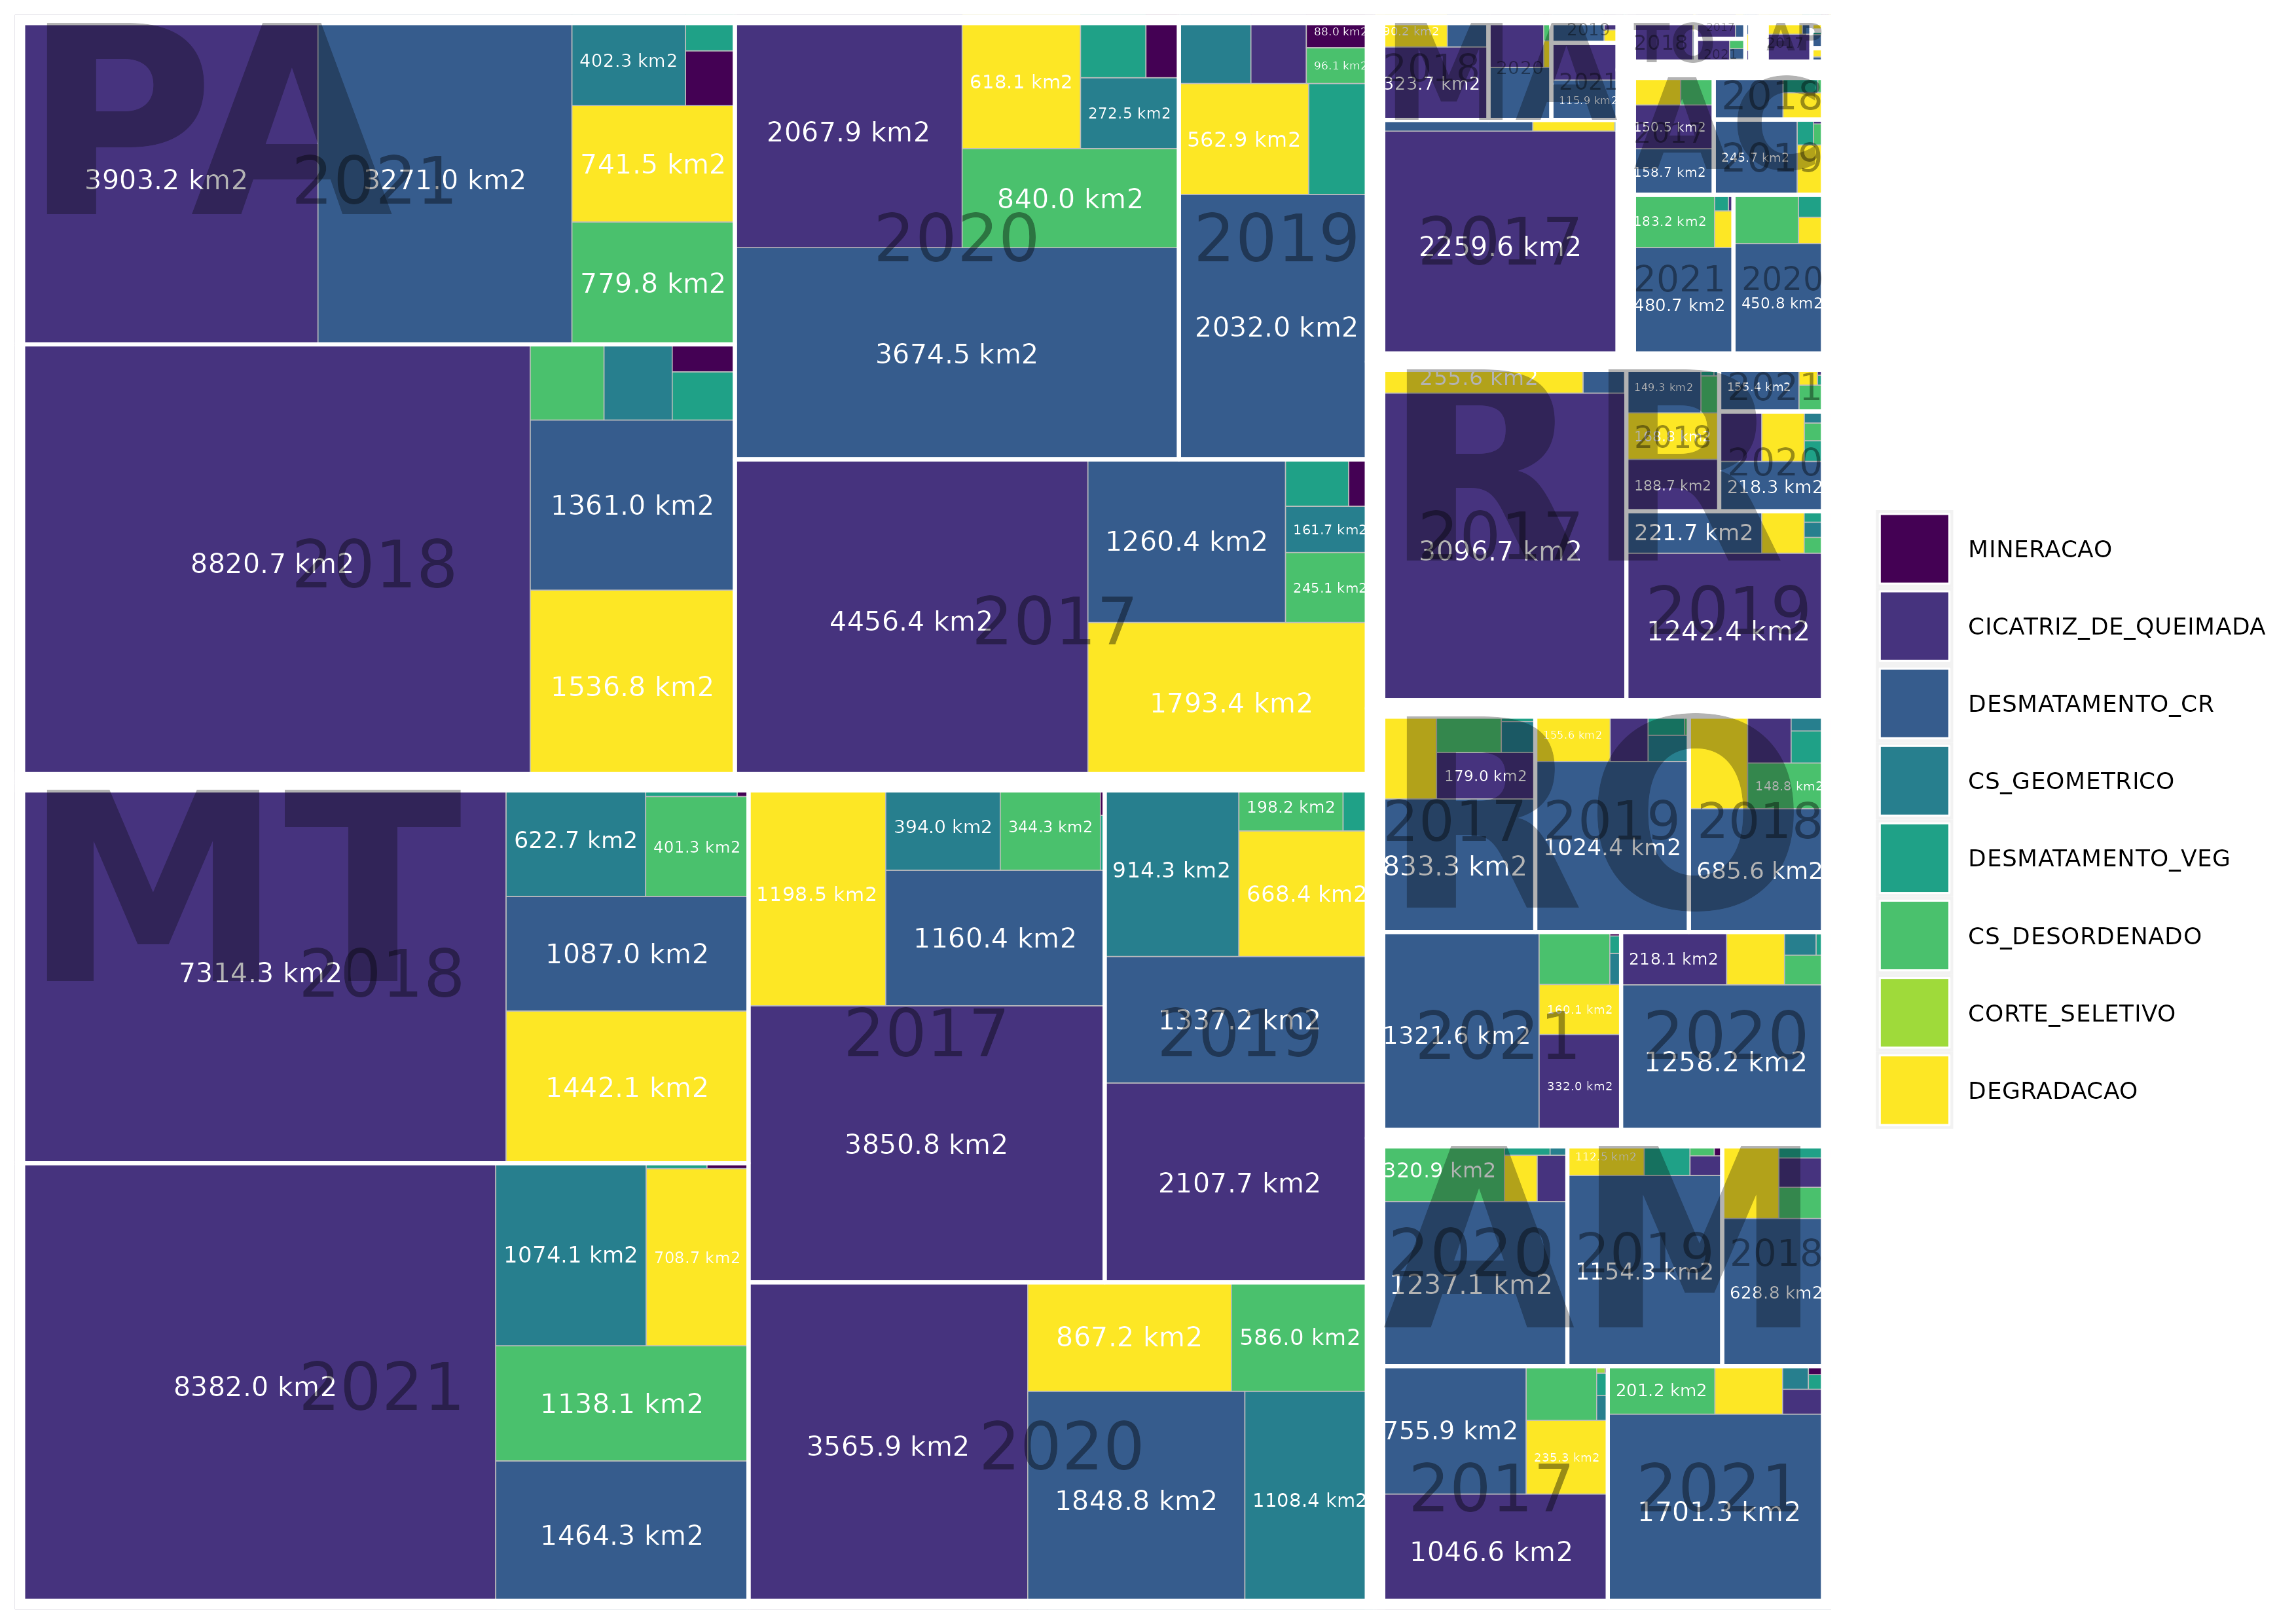
\includegraphics[width=0.75\linewidth]
        {./figures/plot_deter_area_by_state_pyear_type.png}
        \label{fig:deter_area_state_pyear_type}
    \end{figure}
\end{frame}

\begin{frame}
    \frametitle{DETER warnings by class}
    \begin{figure}[h]
        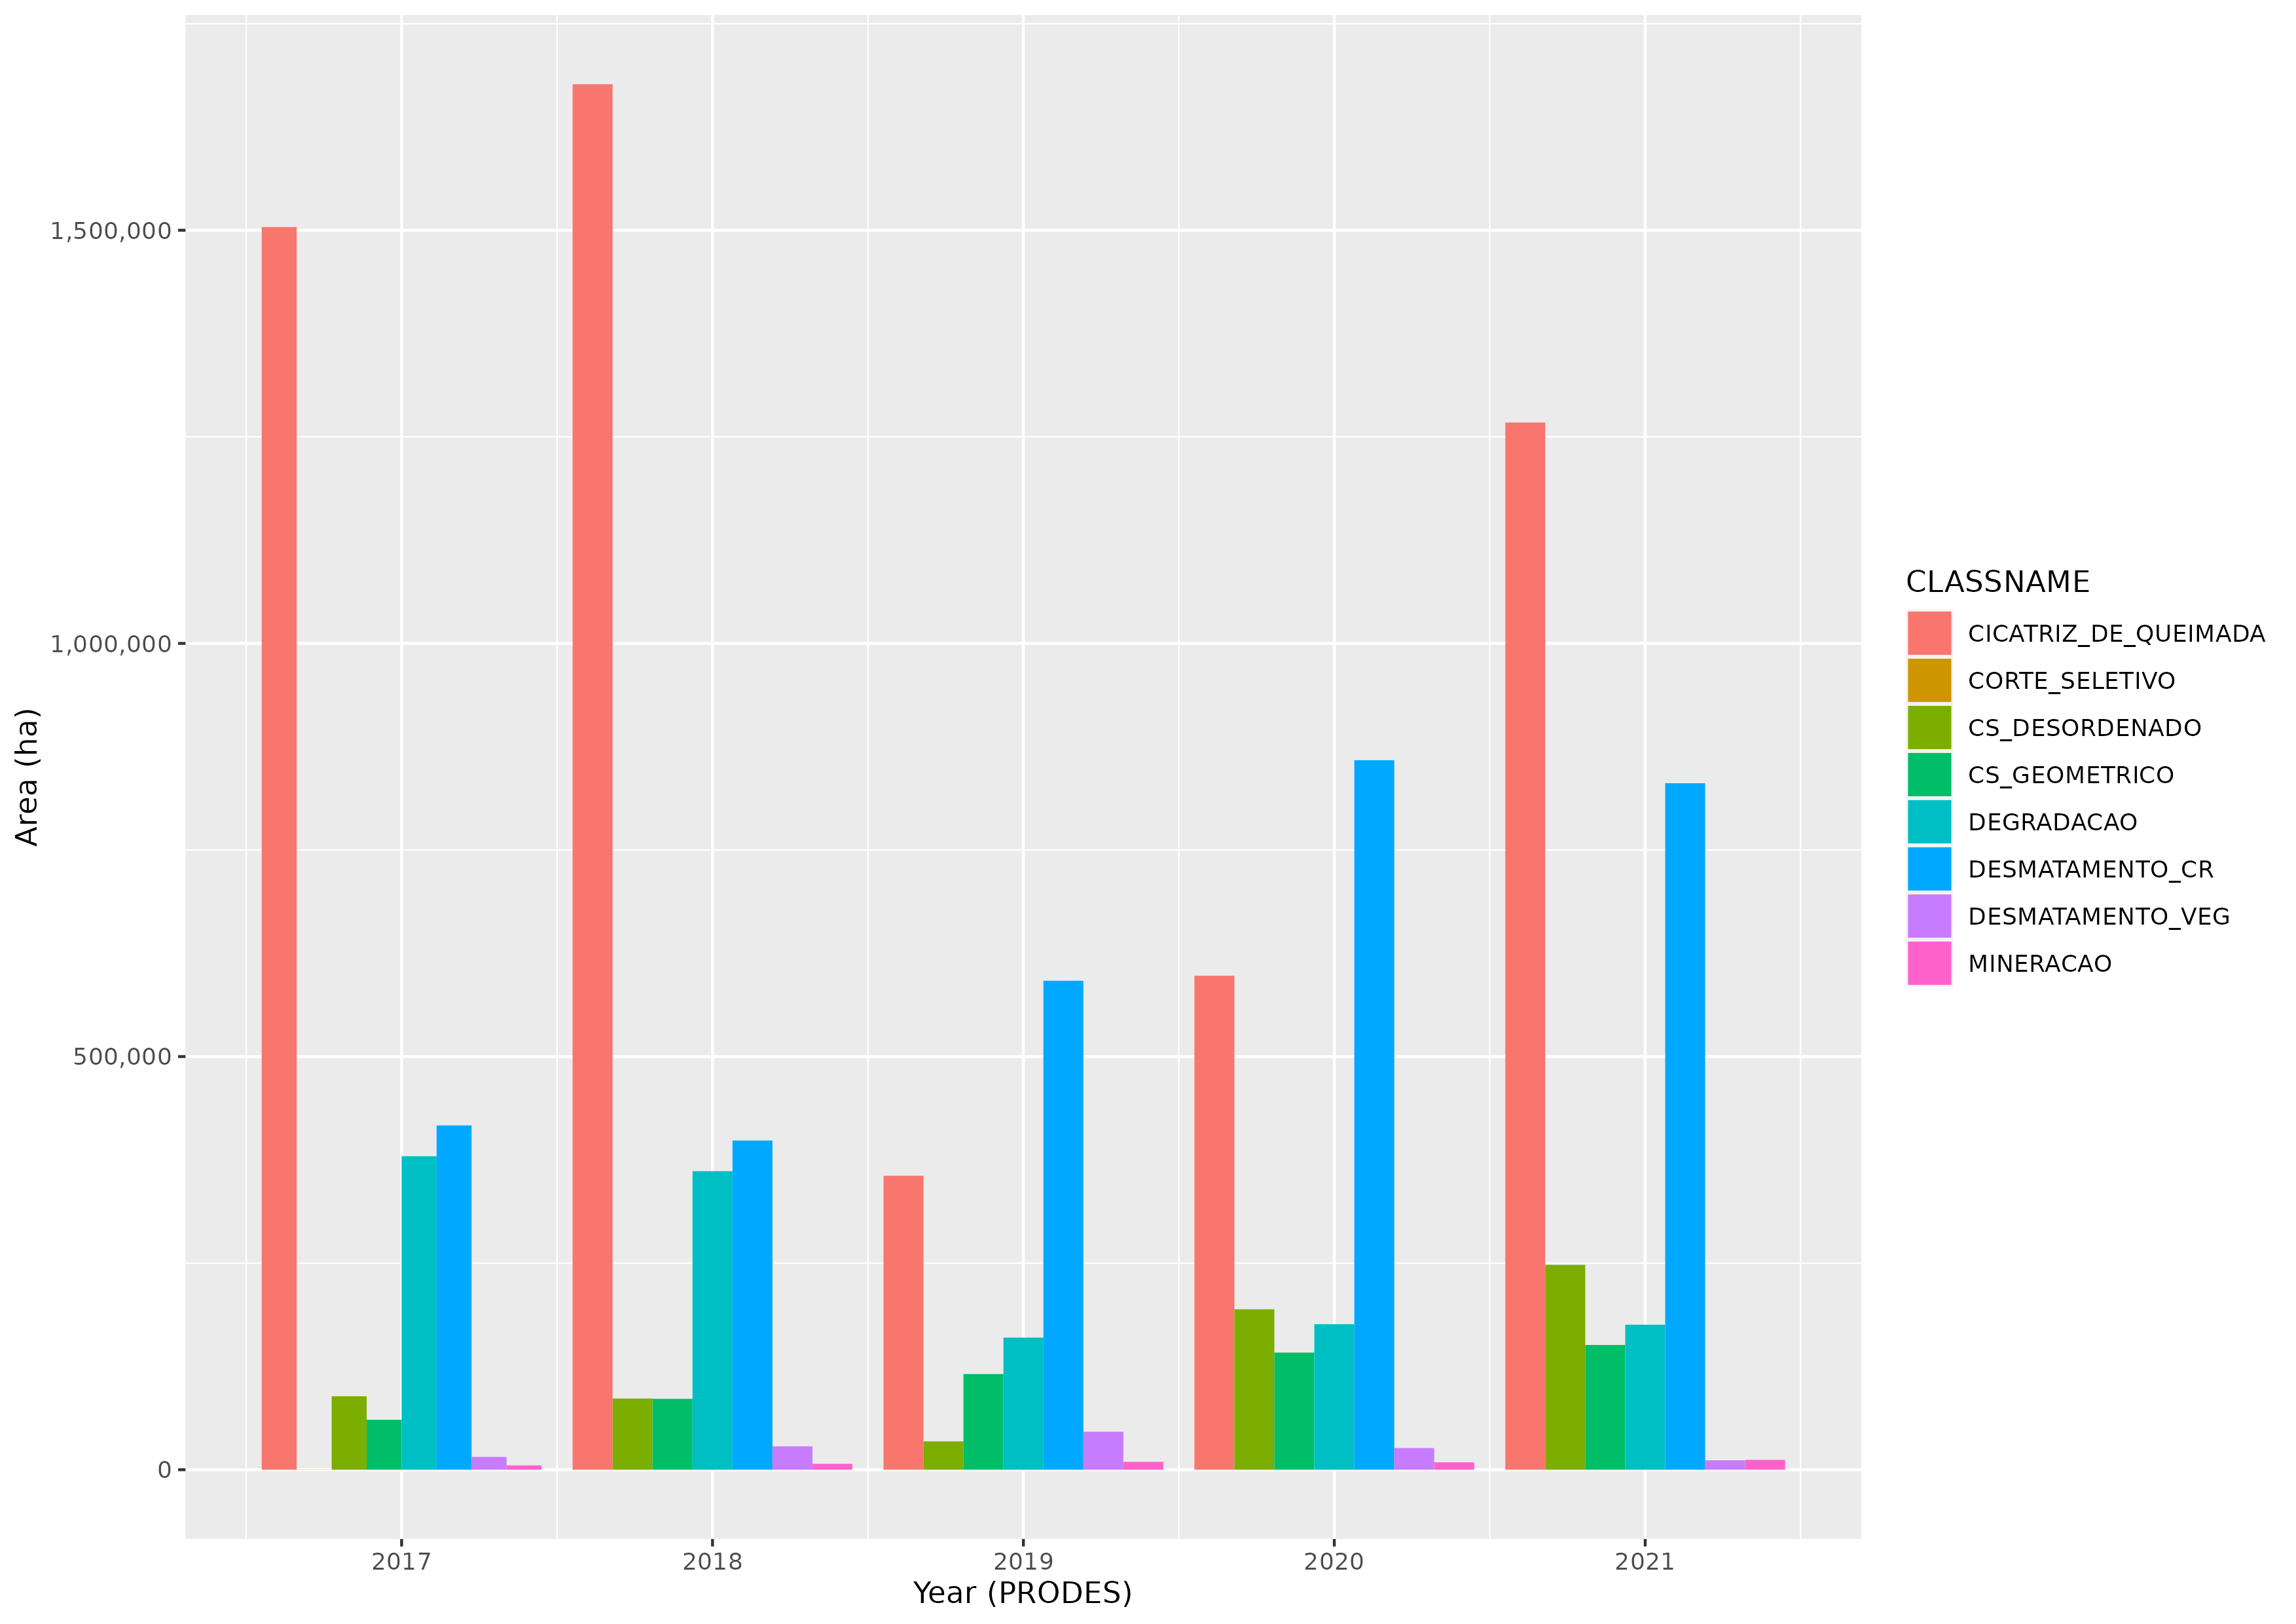
\includegraphics[width=0.65\linewidth]
        {./figures/plot_deter_area_by_class.png}
        \label{fig:deter_area_by_class}
        \caption{Burn scars and clear cut are the most common warnings.}
    \end{figure}
\end{frame}

\begin{frame}
    \frametitle{DETER warnings by class and state}
    \begin{figure}[h]
        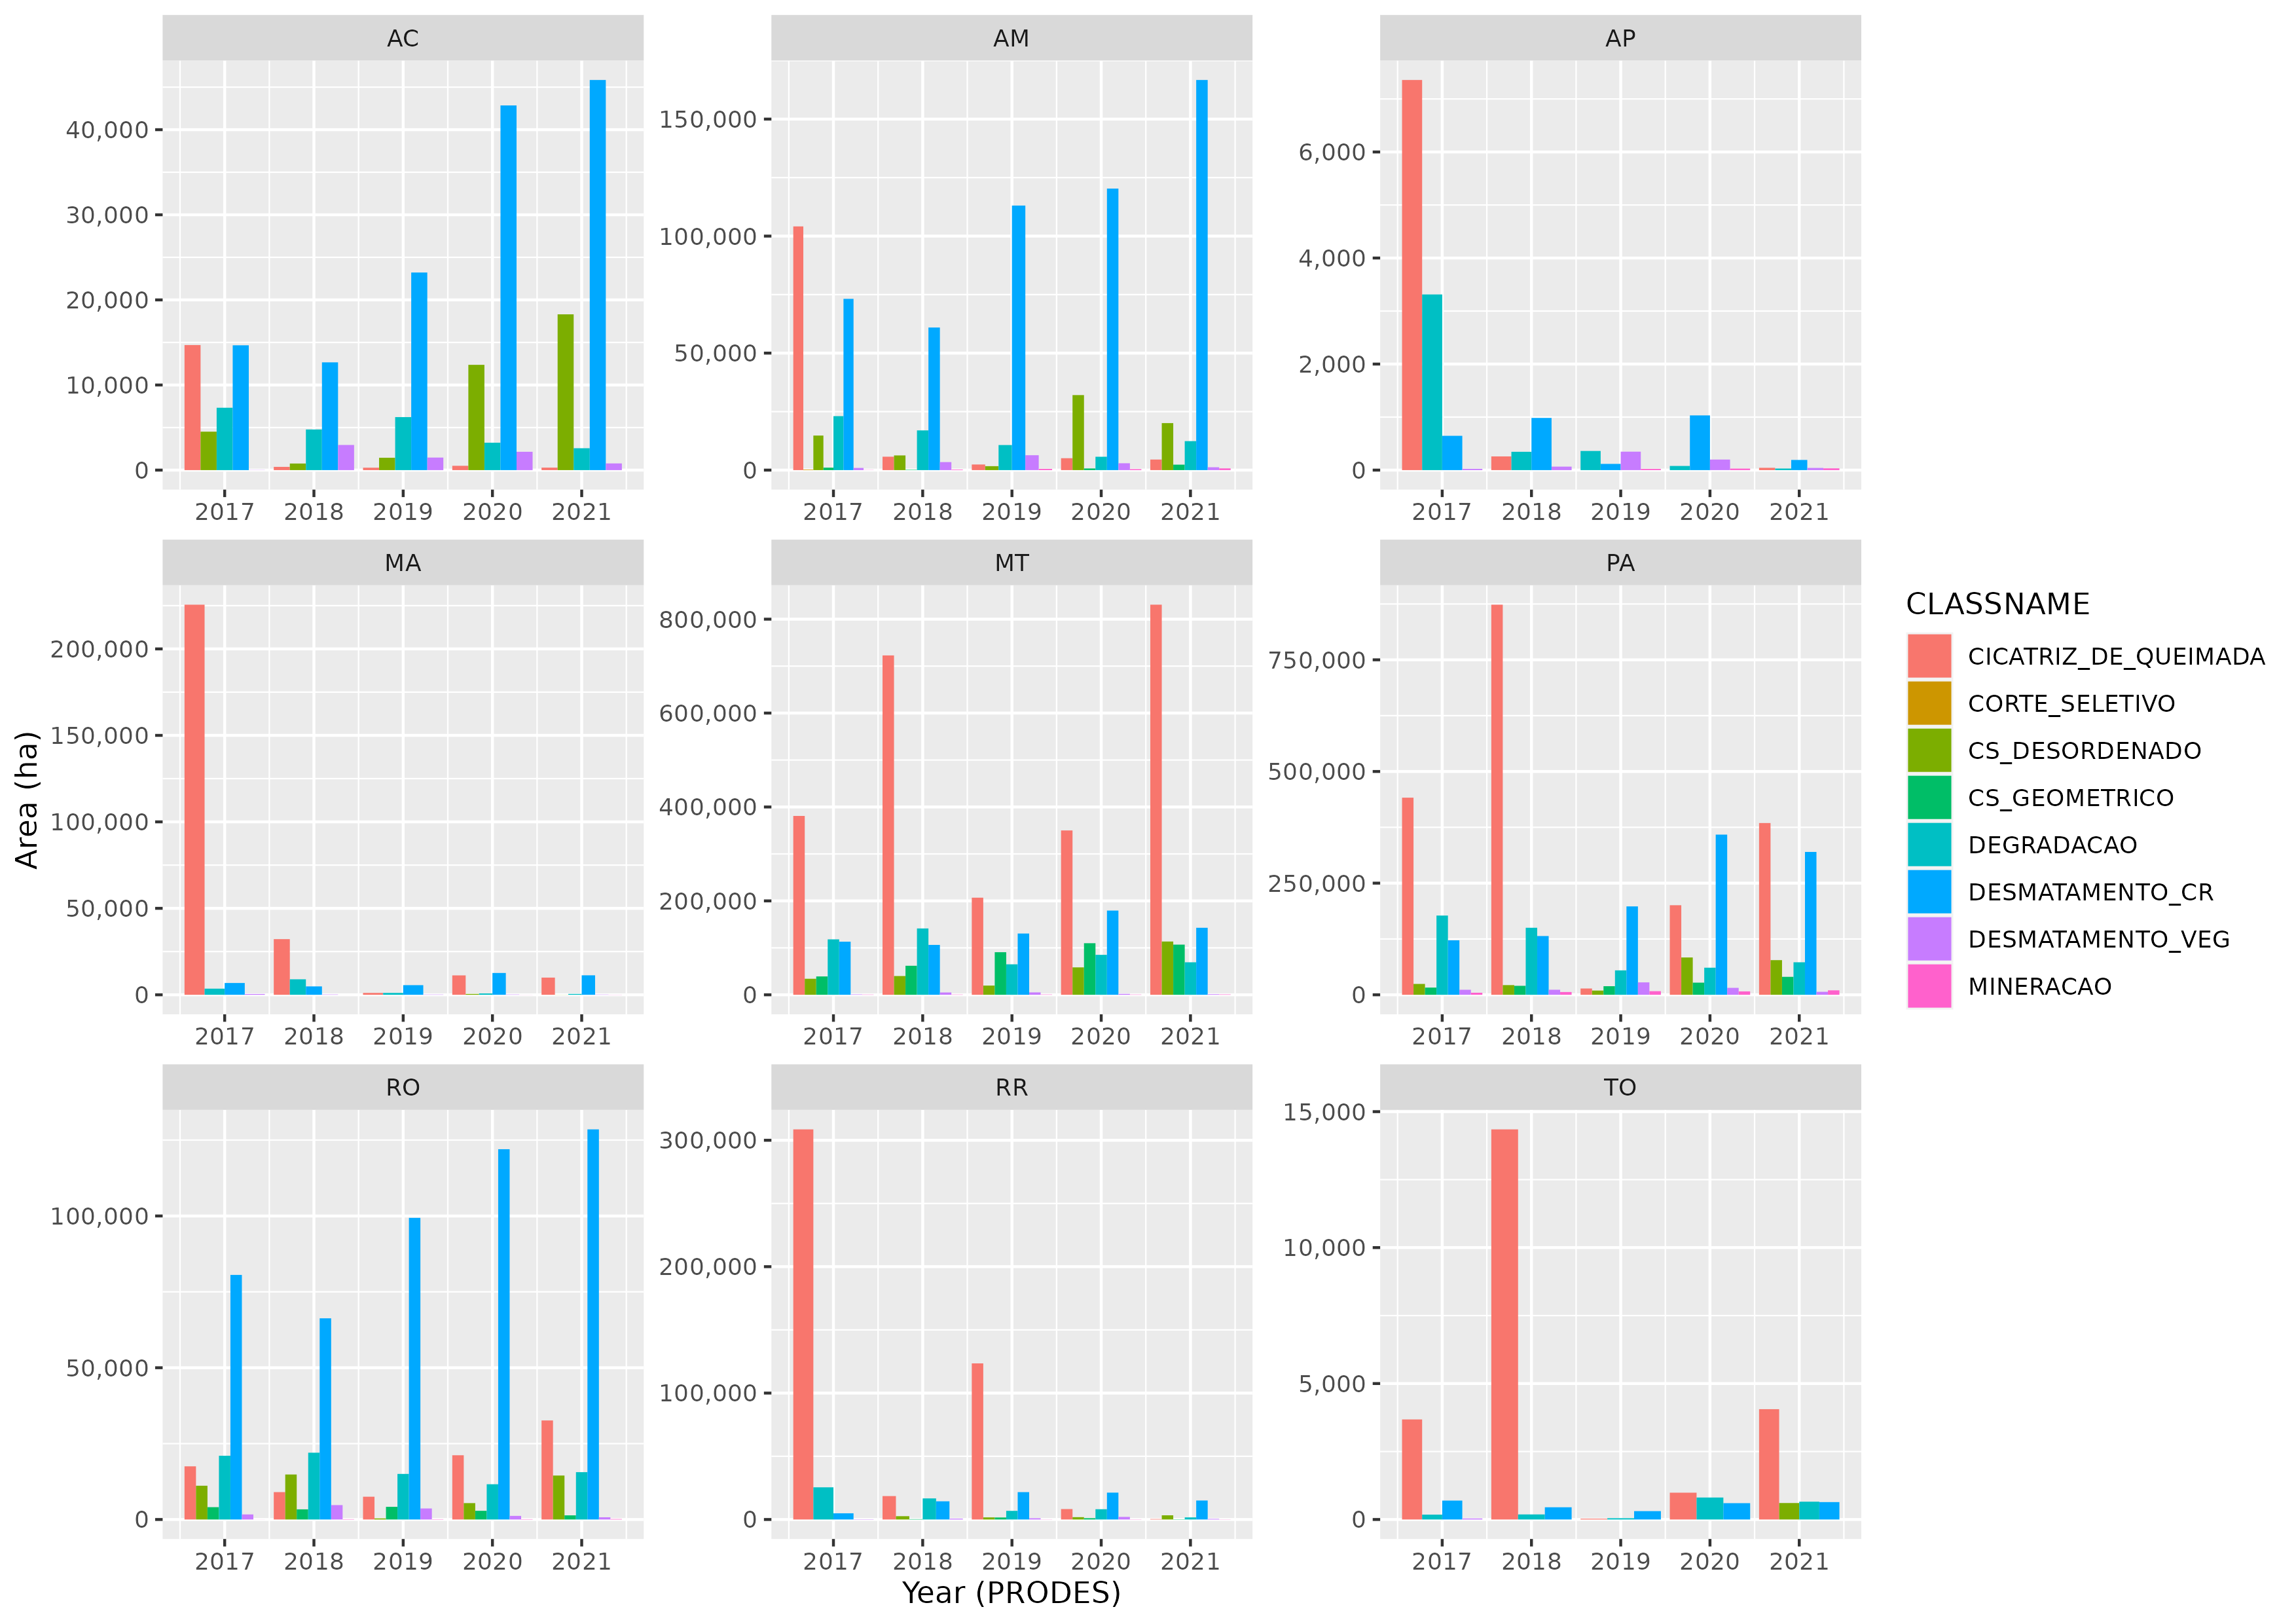
\includegraphics[width=0.65\linewidth]
        {./figures/plot_deter_area_by_class_state.png}
        \label{fig:deter_area_by_class_state}
        \caption{Burn scars and clear cut are the most common warnings.}
    \end{figure}
\end{frame}


\begin{frame}
    \frametitle{DETER warnings and time}
    \begin{itemize}
        \item The spatial properties of DETER warning are inconsistent along 
            time (shape, size, position, orientation).
    \end{itemize}
\end{frame}

\begin{frame}
    \frametitle{Warnings are inconsistent along time}
    \begin{figure}[h] 
        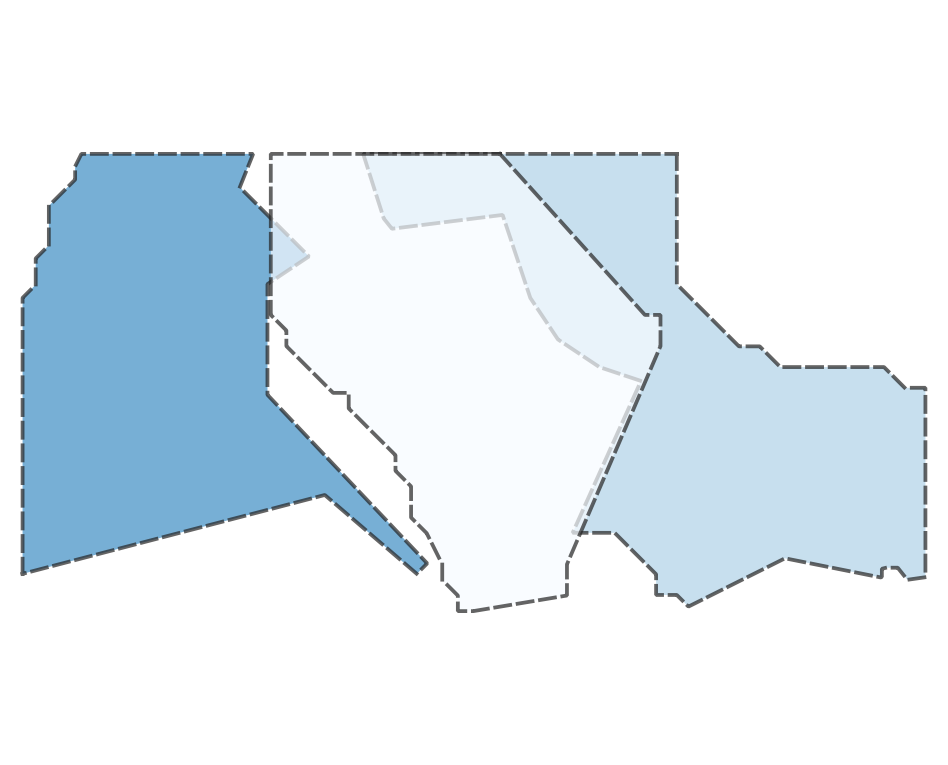
\includegraphics[width=0.60\linewidth]
        {./images/sample_deter_warnings.png}
        \label{fig:deter_subareas}
        \caption{DETER warnings don't fit along time.}
    \end{figure}
\end{frame}



\subsection{DETER subareas}

\begin{frame}
    \frametitle{DETER subareas}
    \begin{itemize}
        \item The spatial properties of DETER warning are inconsistent along 
            time (shape, size, position, orientation).
        \item DETER subareas maintain their spatial properties along time.
    \end{itemize}
\end{frame}

\begin{frame}
    \frametitle{DETER subareas}
    \begin{figure}[h] 
        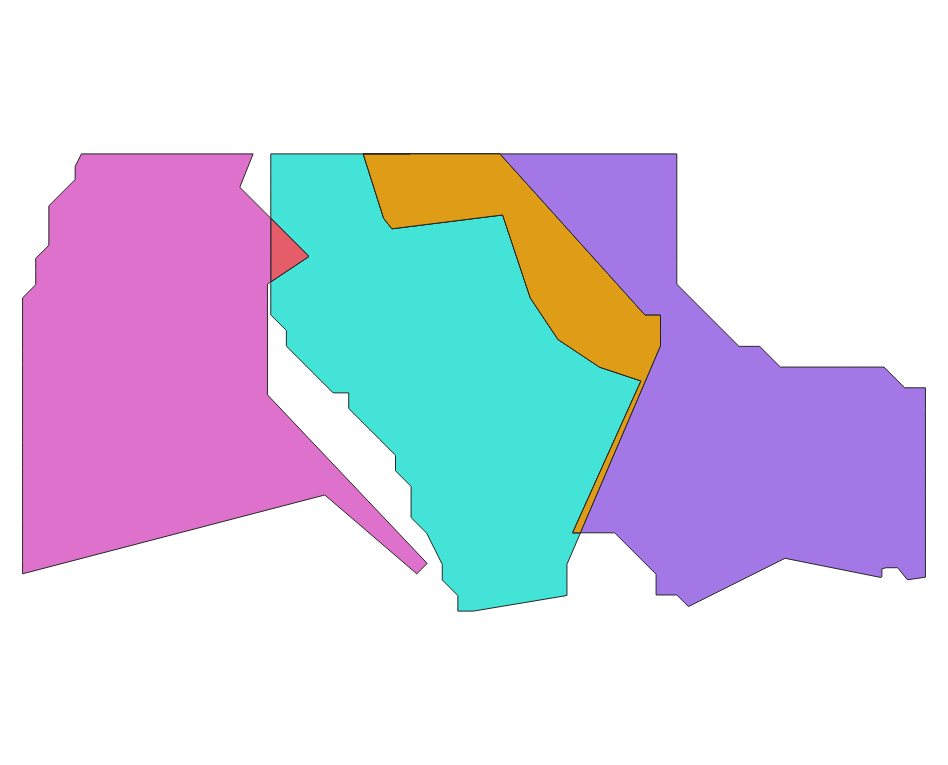
\includegraphics[width=0.60\linewidth]
        {./images/sample_deter_subareas.png}
        \caption{From 3 DETER warnings, we get 7 subareas!}
        \label{fig:deter_subareas}
    \end{figure}
\end{frame}





\section{DETER subareas EDA}

\begin{frame}
    \frametitle{DETER subareas}
    \begin{figure}[h] 
        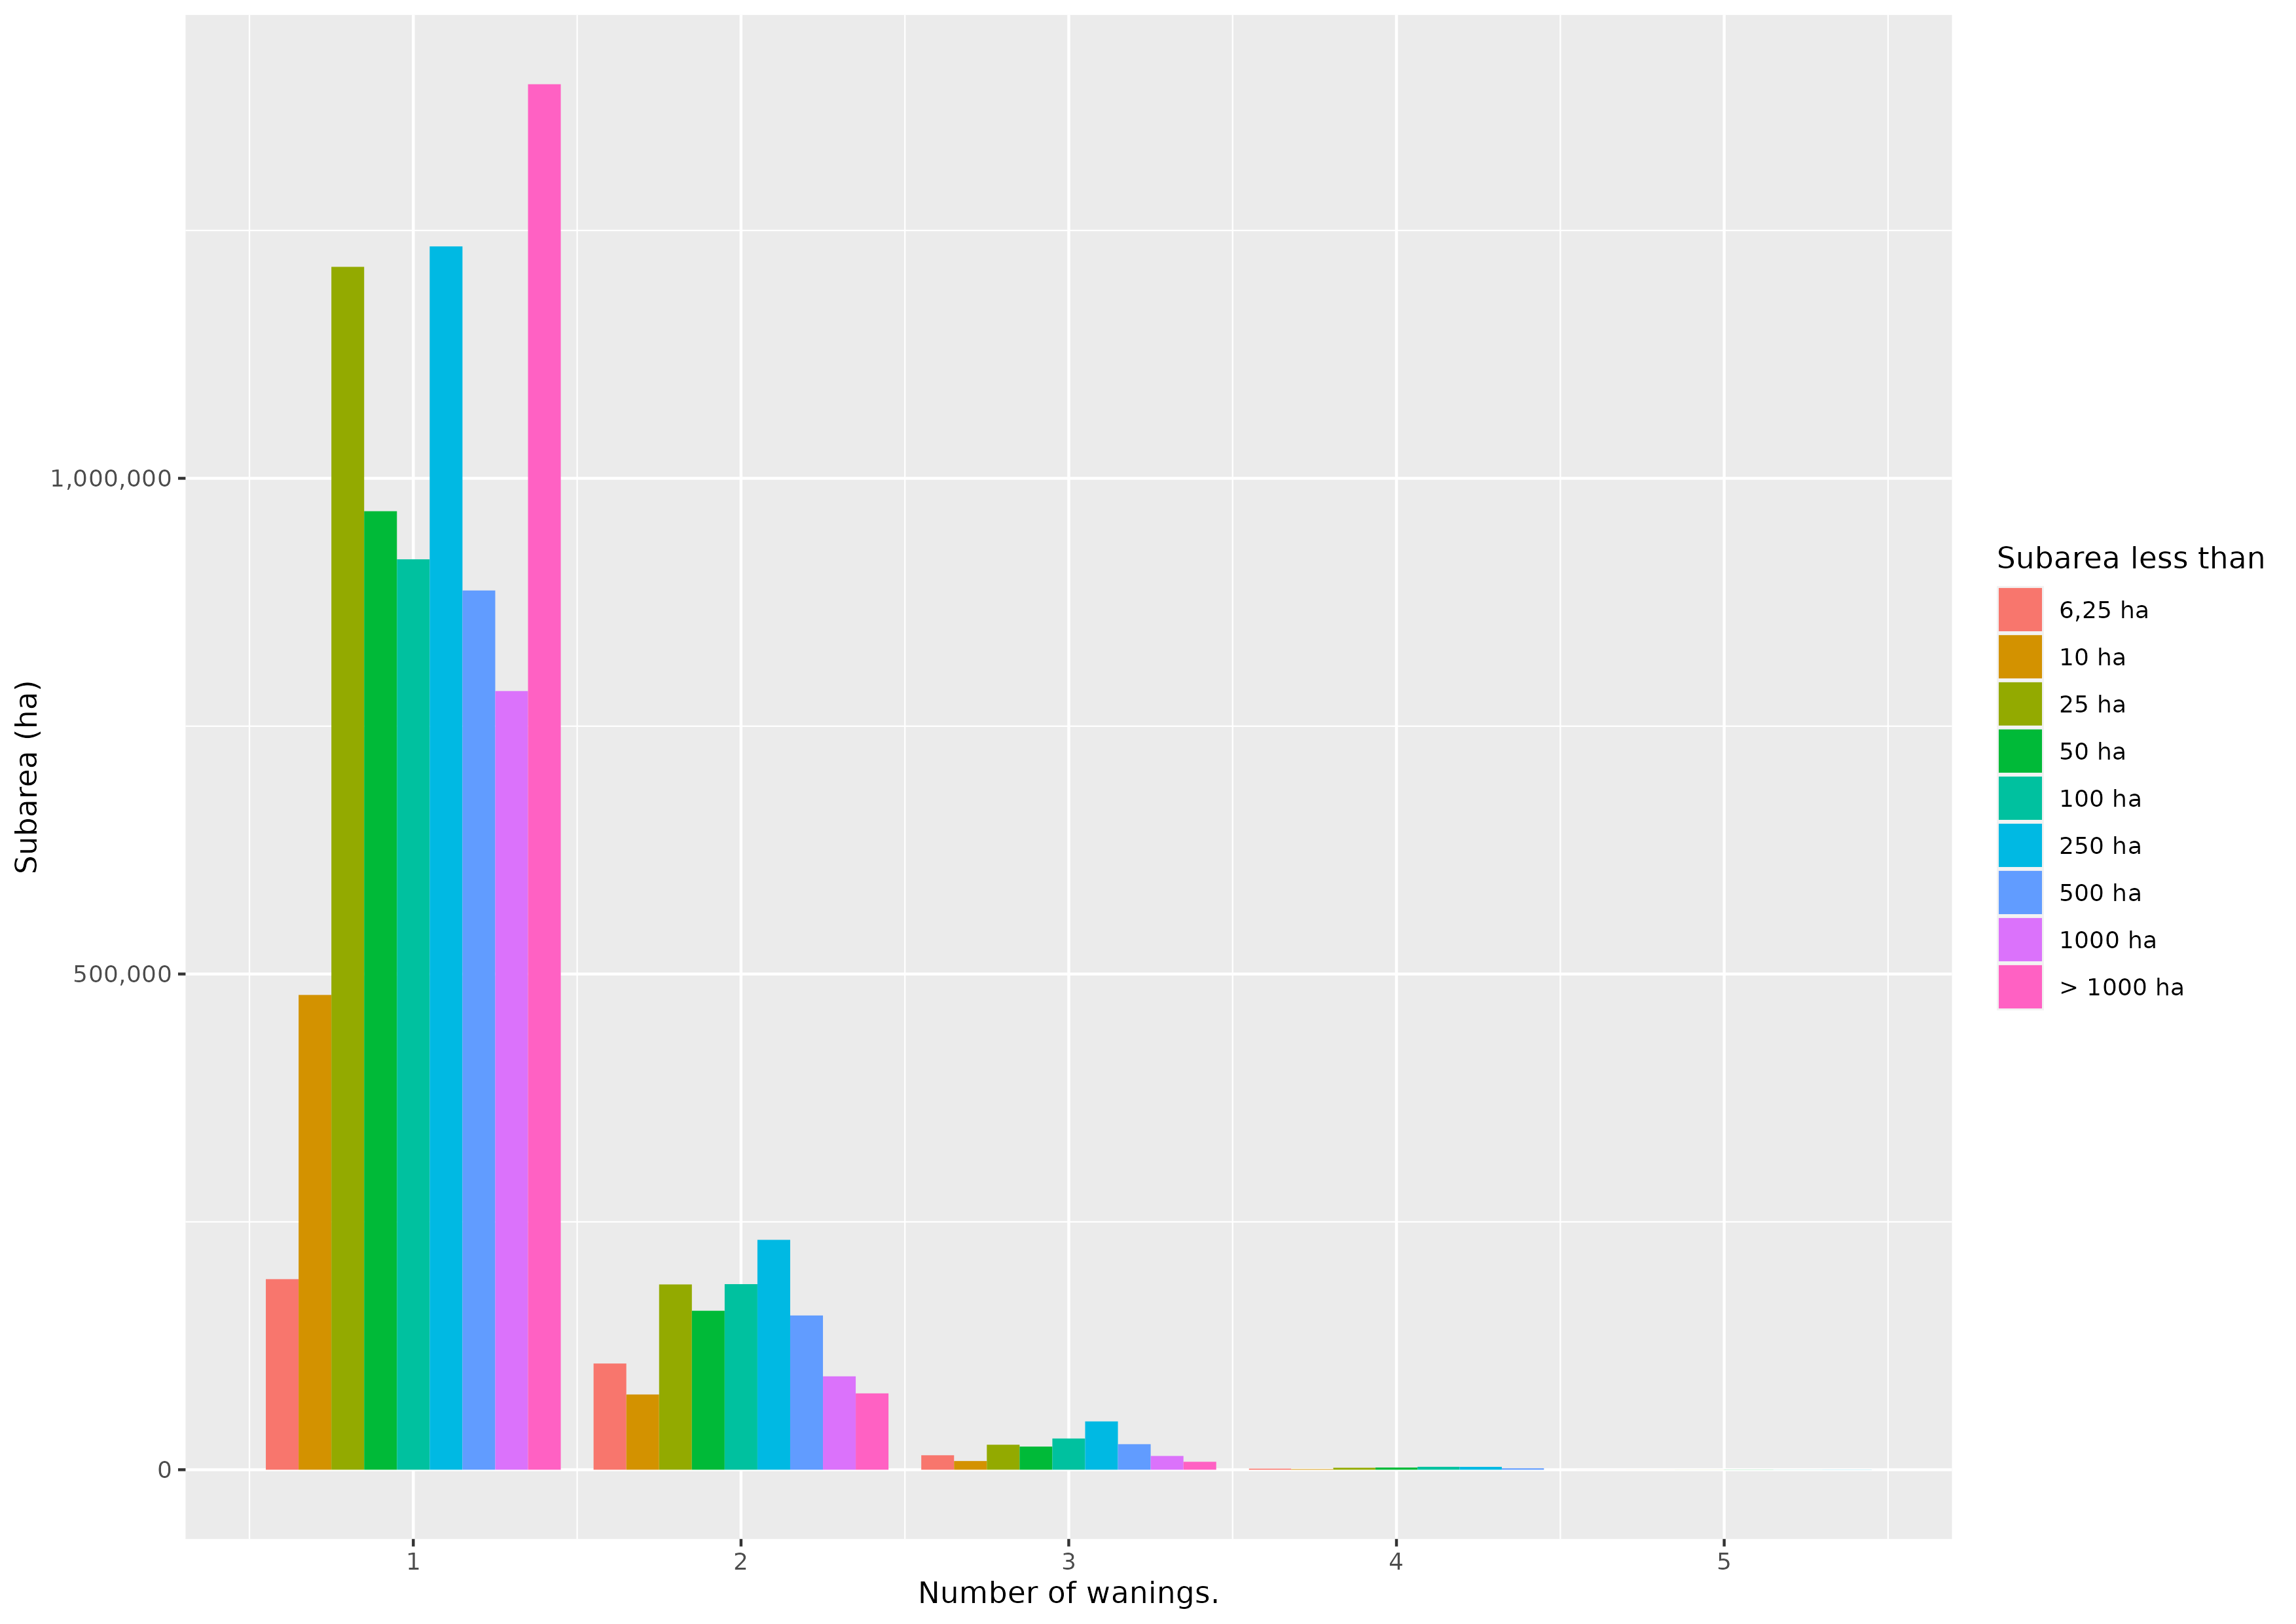
\includegraphics[width=0.65\linewidth]
        {./figures/plot_deter_subarea_by_nwarnings.png}
        \caption{There are subareas with up to 5 recurrent warnings.}
        \label{fig:deter_subareas_nwarnings}
    \end{figure}
\end{frame}

\begin{frame}
    \frametitle{DETER subareas}
    \begin{figure}[h] 
        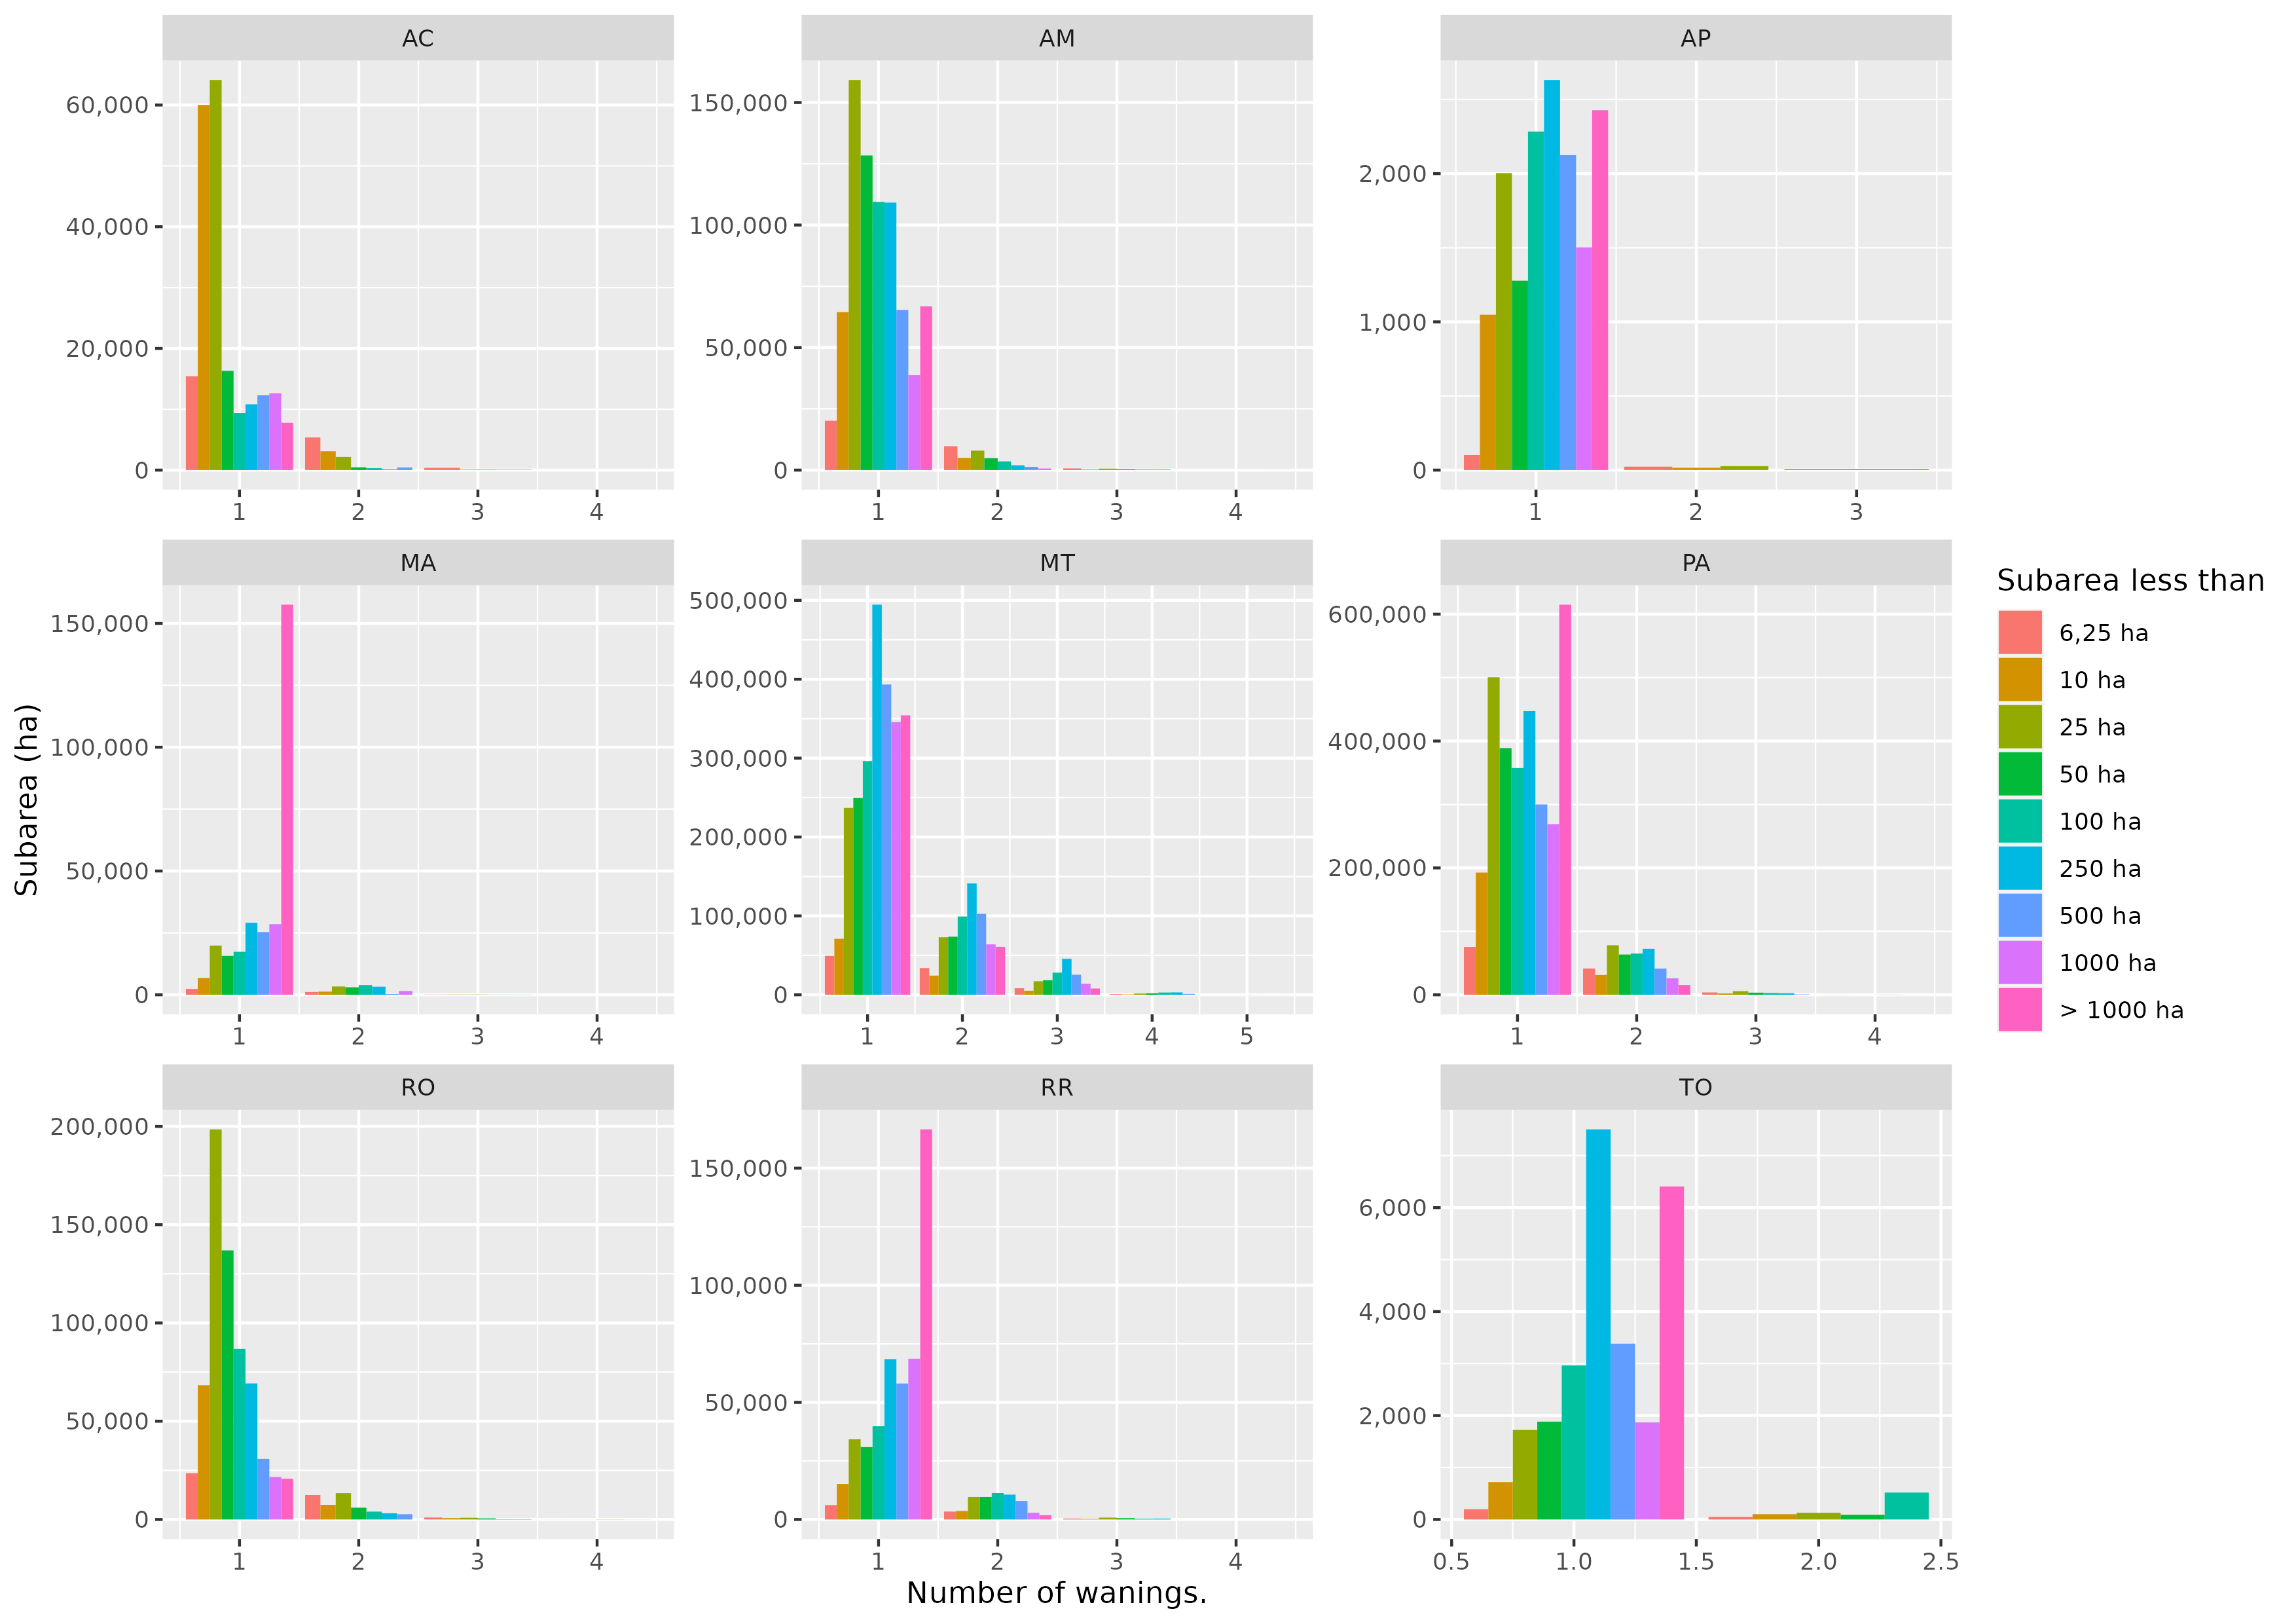
\includegraphics[width=0.65\linewidth]
        {./figures/plot_deter_subarea_by_warnings_state.png}
        \caption{The warning recurrence changes by brazilian state.}
        \label{fig:deter_subarea_warnings_state}
    \end{figure}
\end{frame}

\begin{frame}
    \frametitle{DETER subareas}
    \begin{figure}[h] 
        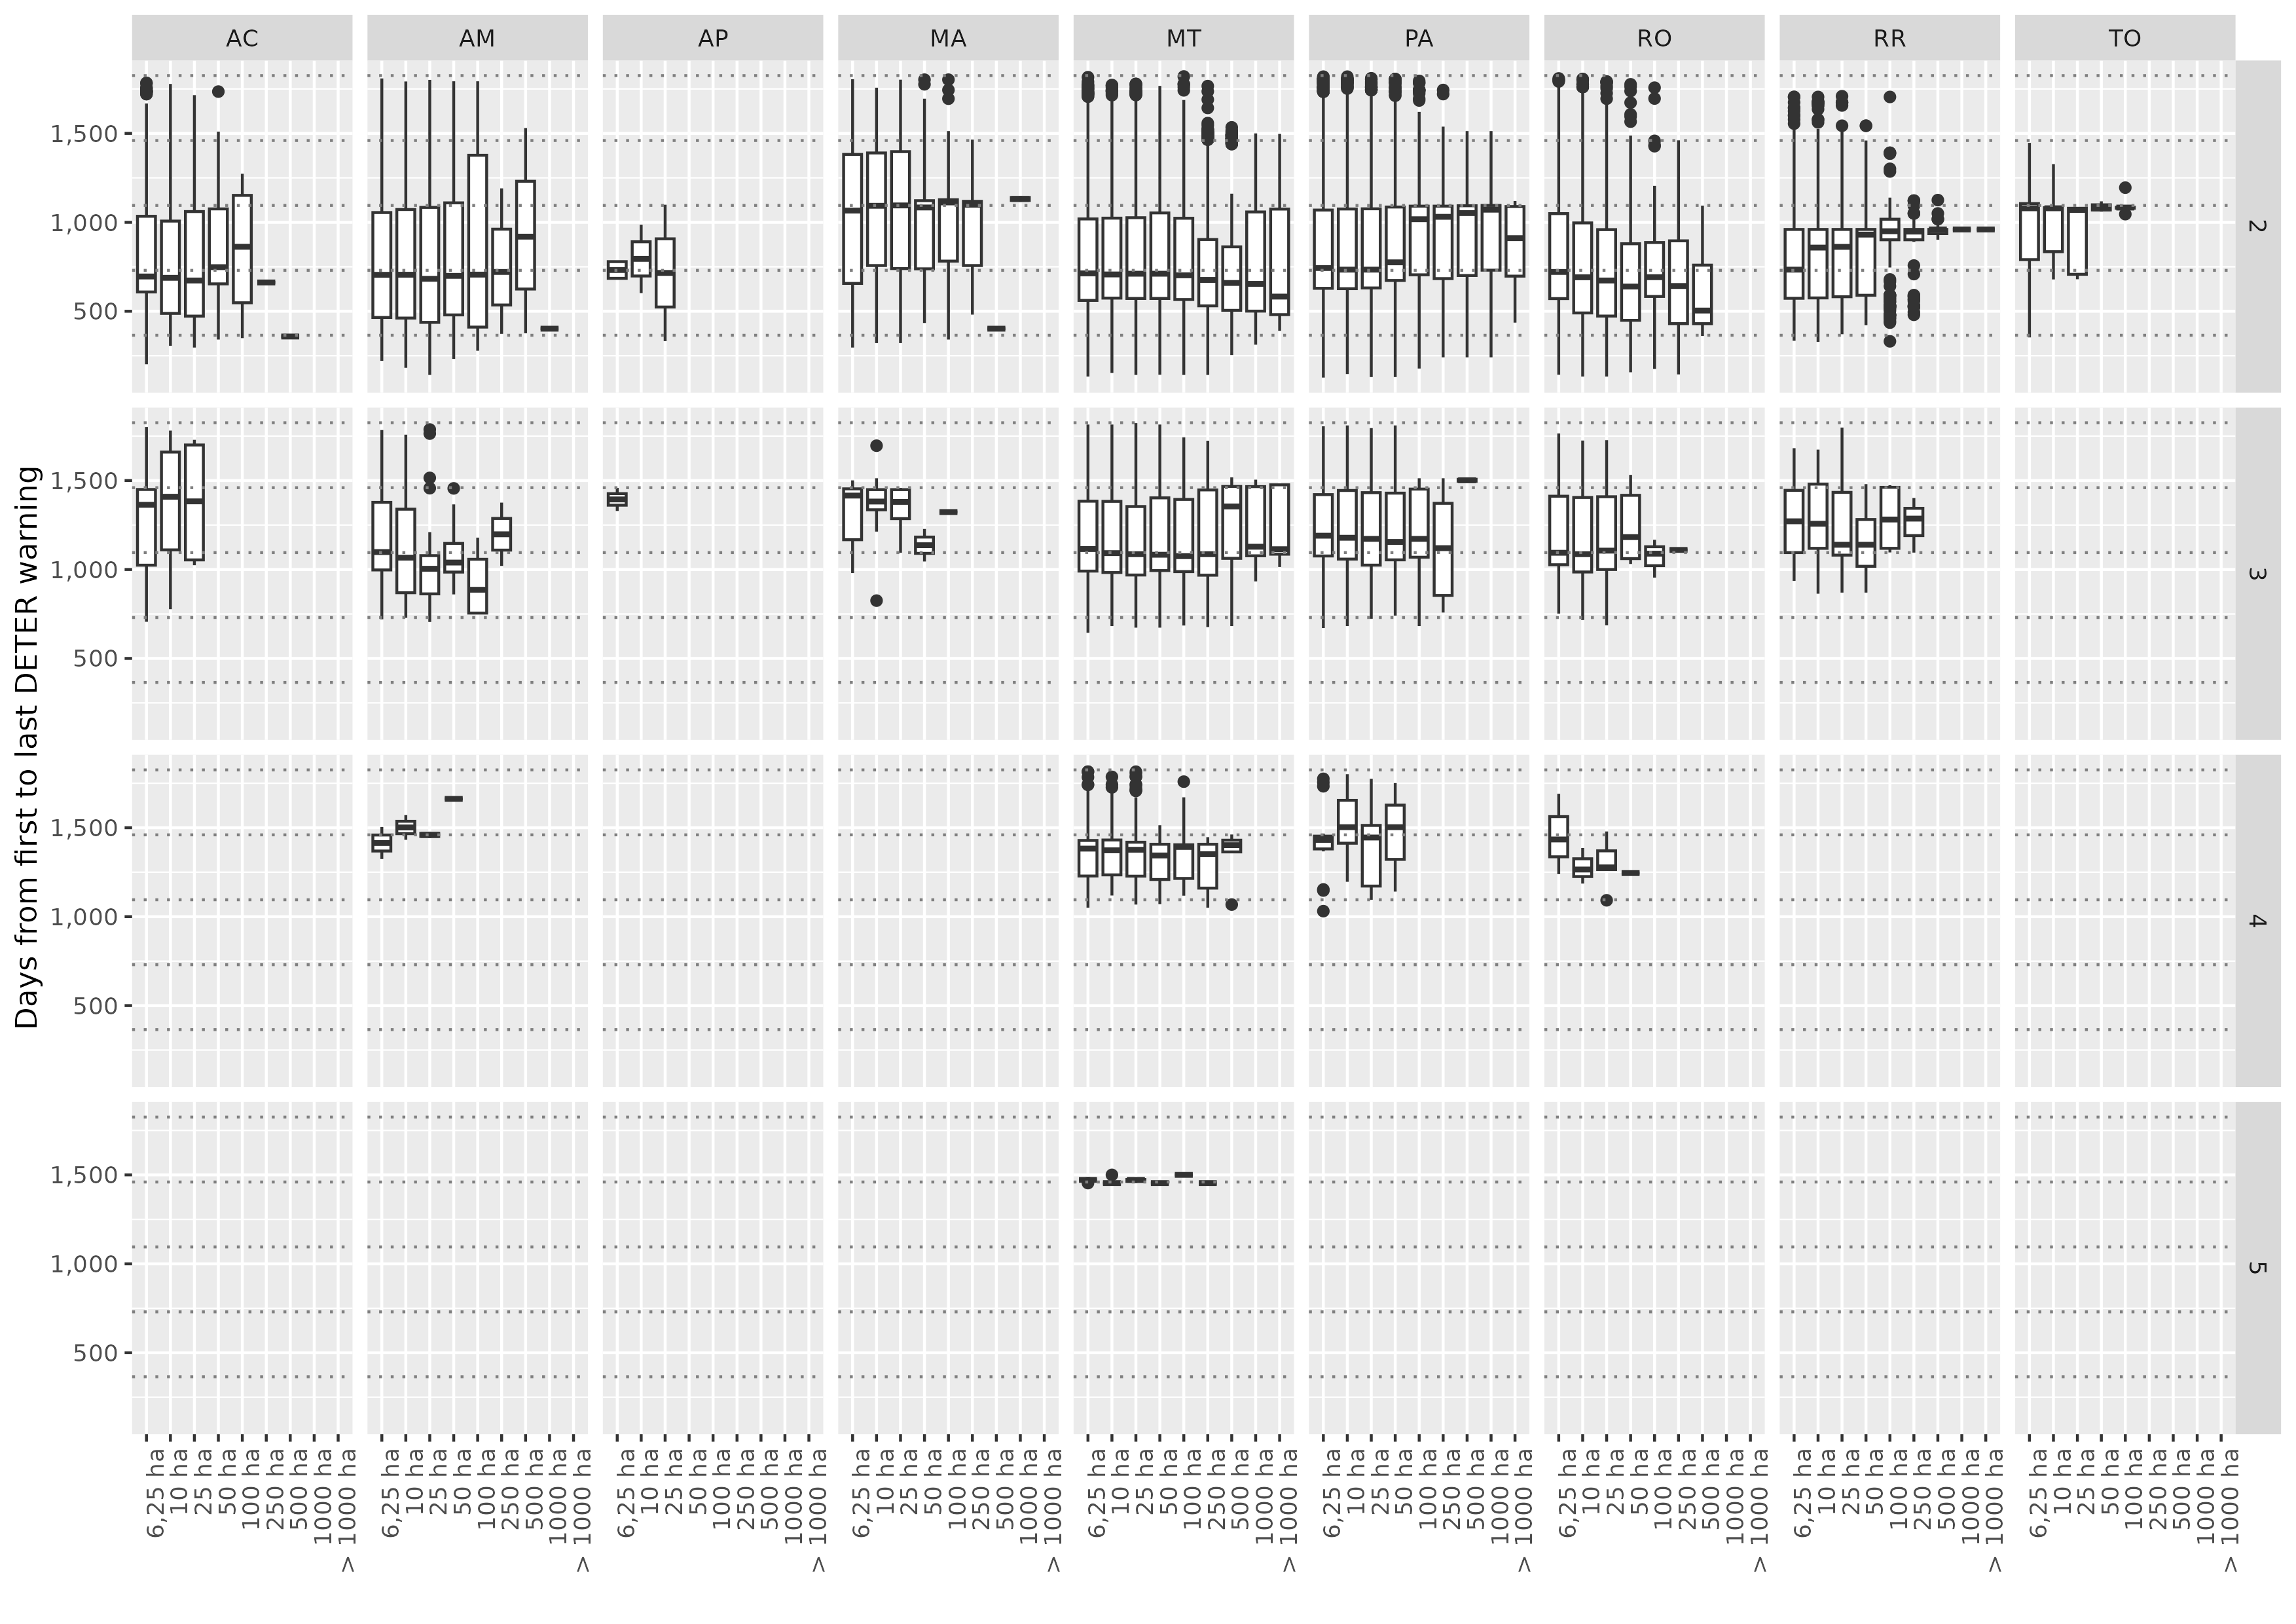
\includegraphics[width=0.65\linewidth]
        {./figures/plot_deter_days_first_to_last.png}
        \caption{Number of days between first and last warning.}
        \label{fig:deter_days_first_to_last}
    \end{figure}
\end{frame}

\begin{frame}
    \frametitle{DETER subareas}
    \begin{figure}[h] 
        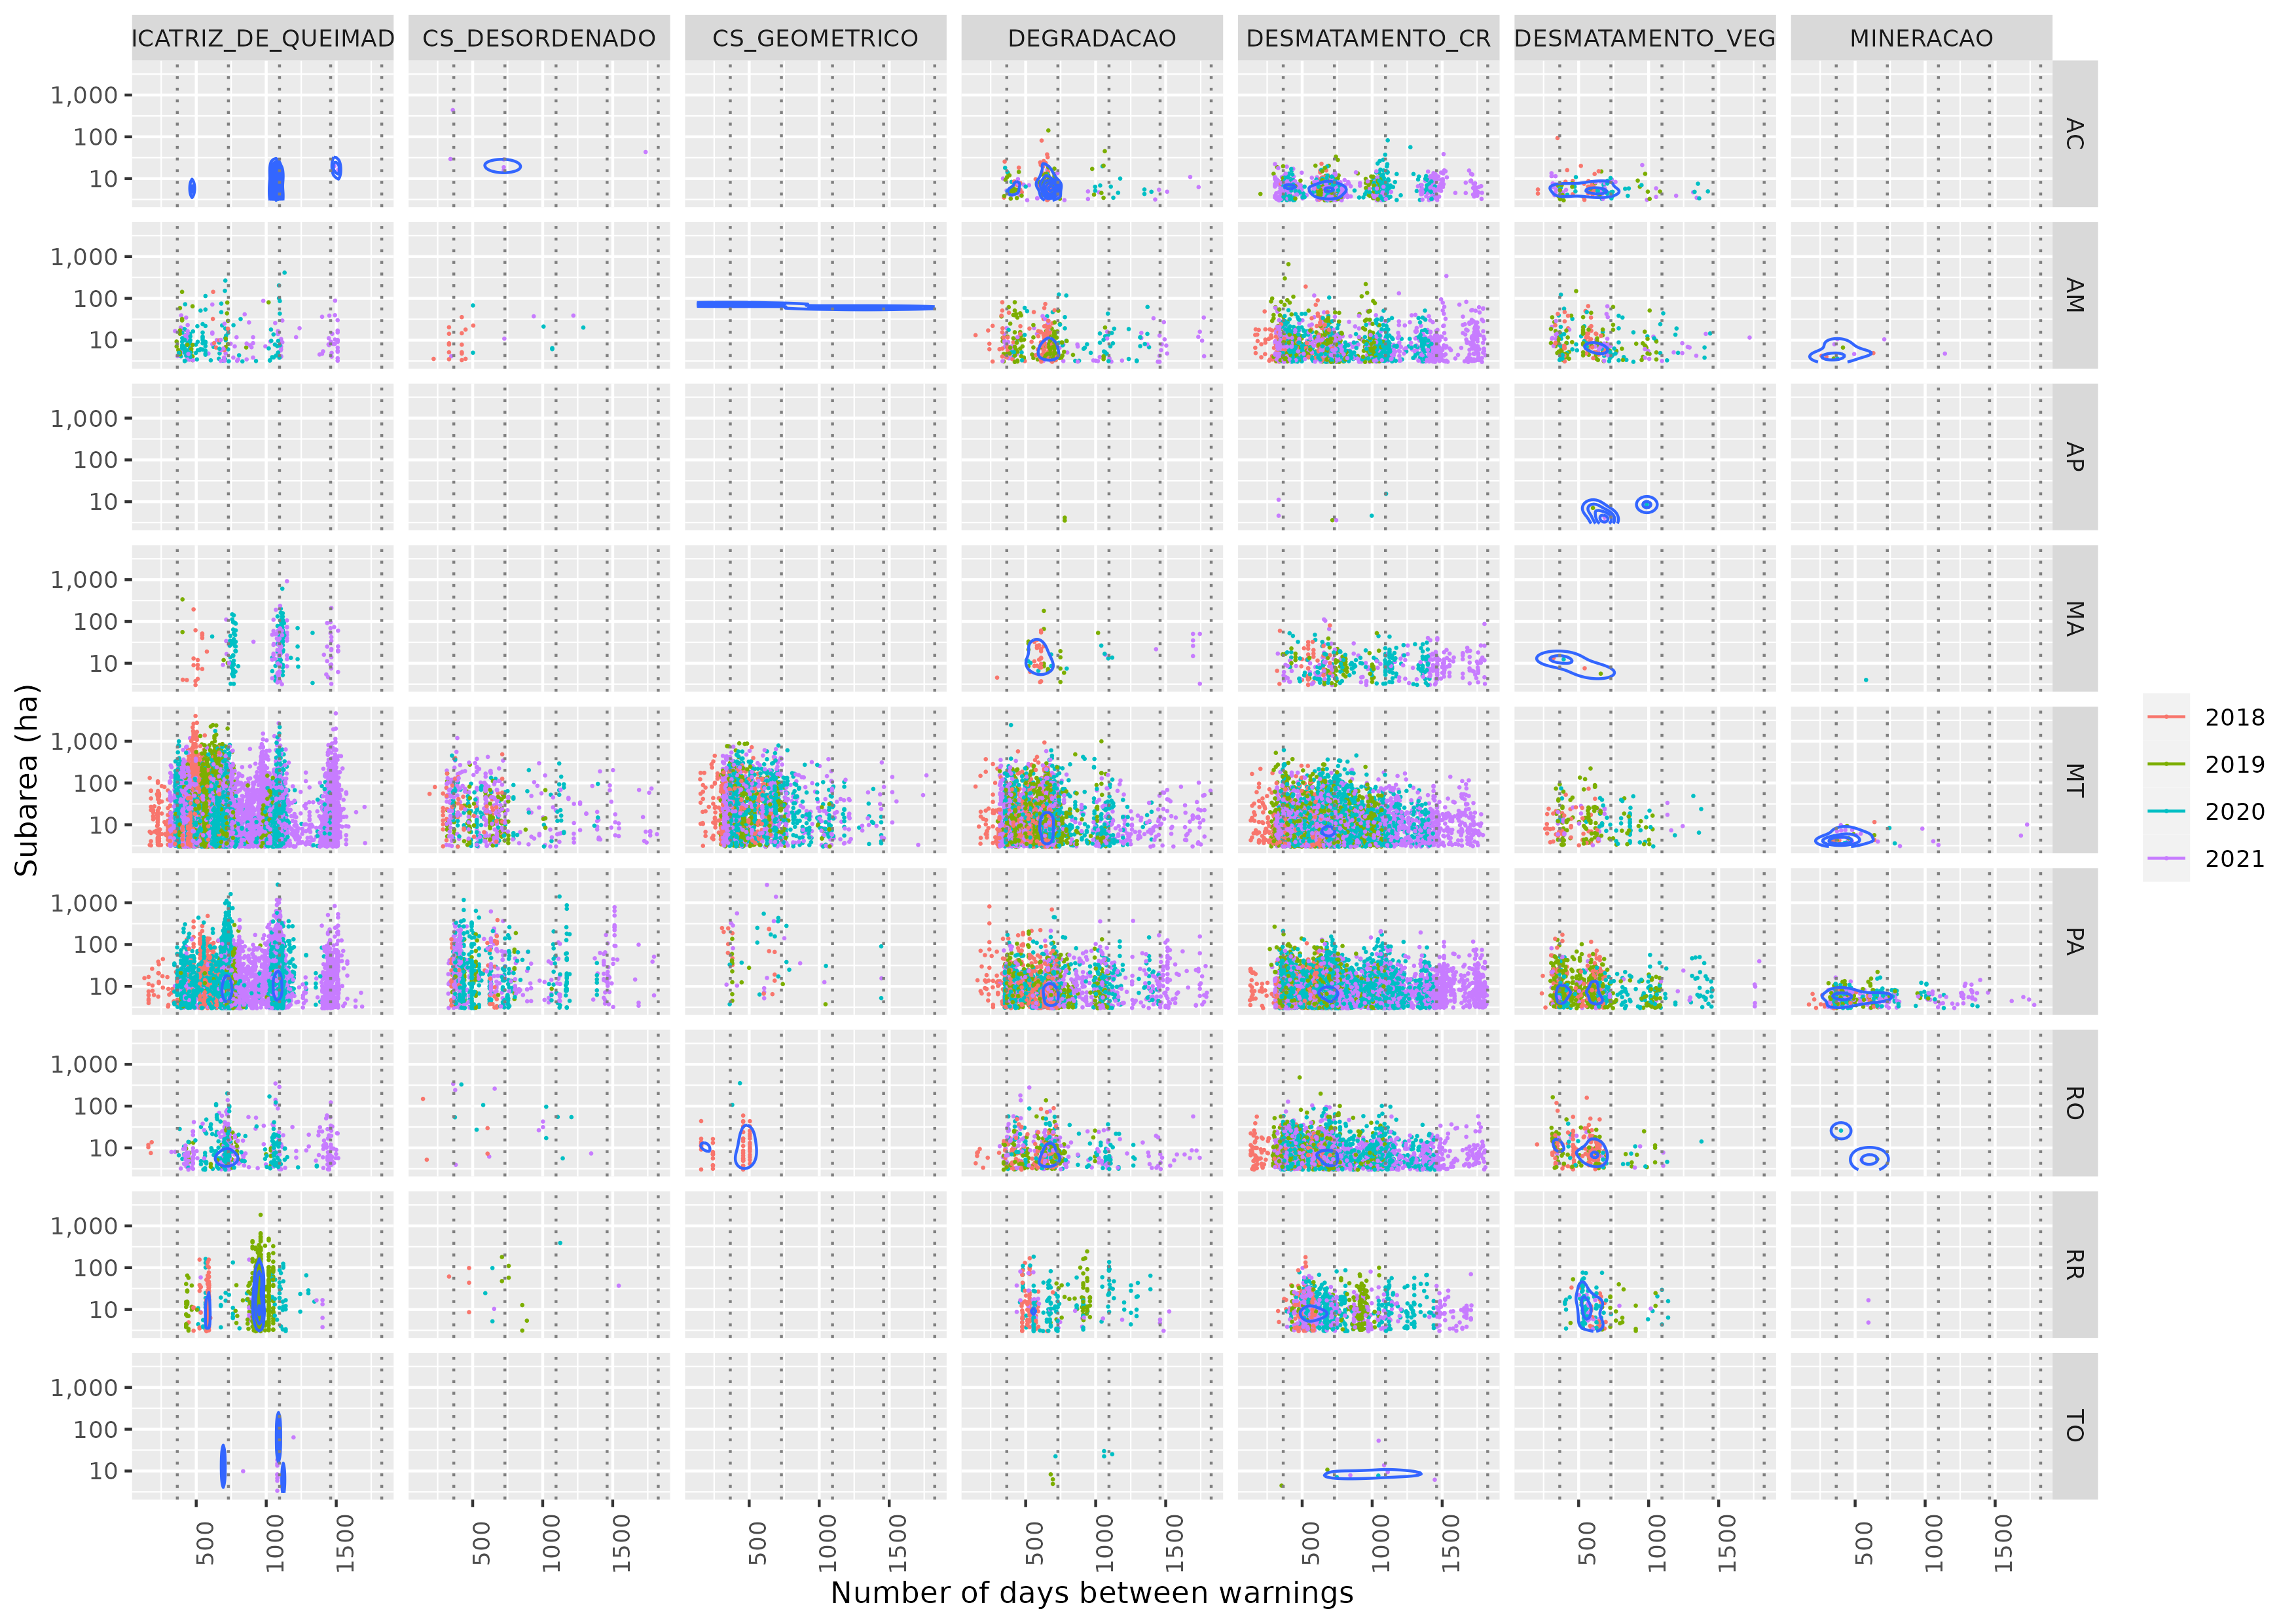
\includegraphics[width=0.65\linewidth]
        {./figures/plot_deter_subarea_density_by_state_first-type_nwarnings.png}
        \caption{The number of days between warnings behavious in space and 
        time.}
        \label{fig:deter_subarea_density_state_first_type_nwarnings}
    \end{figure}
\end{frame}





\section{Subareas trajectories} 

\begin{frame}
    \frametitle{Subarea trajectories}
    \begin{itemize}
        \item Overlaped subareas organized along time describe trajectories of
            change.
    \end{itemize}
\end{frame}


\subsection{Trajectories (DETER)} 

\begin{frame}
    \frametitle{DETER subareas (2 warnings)}
    \begin{figure}[h] 
        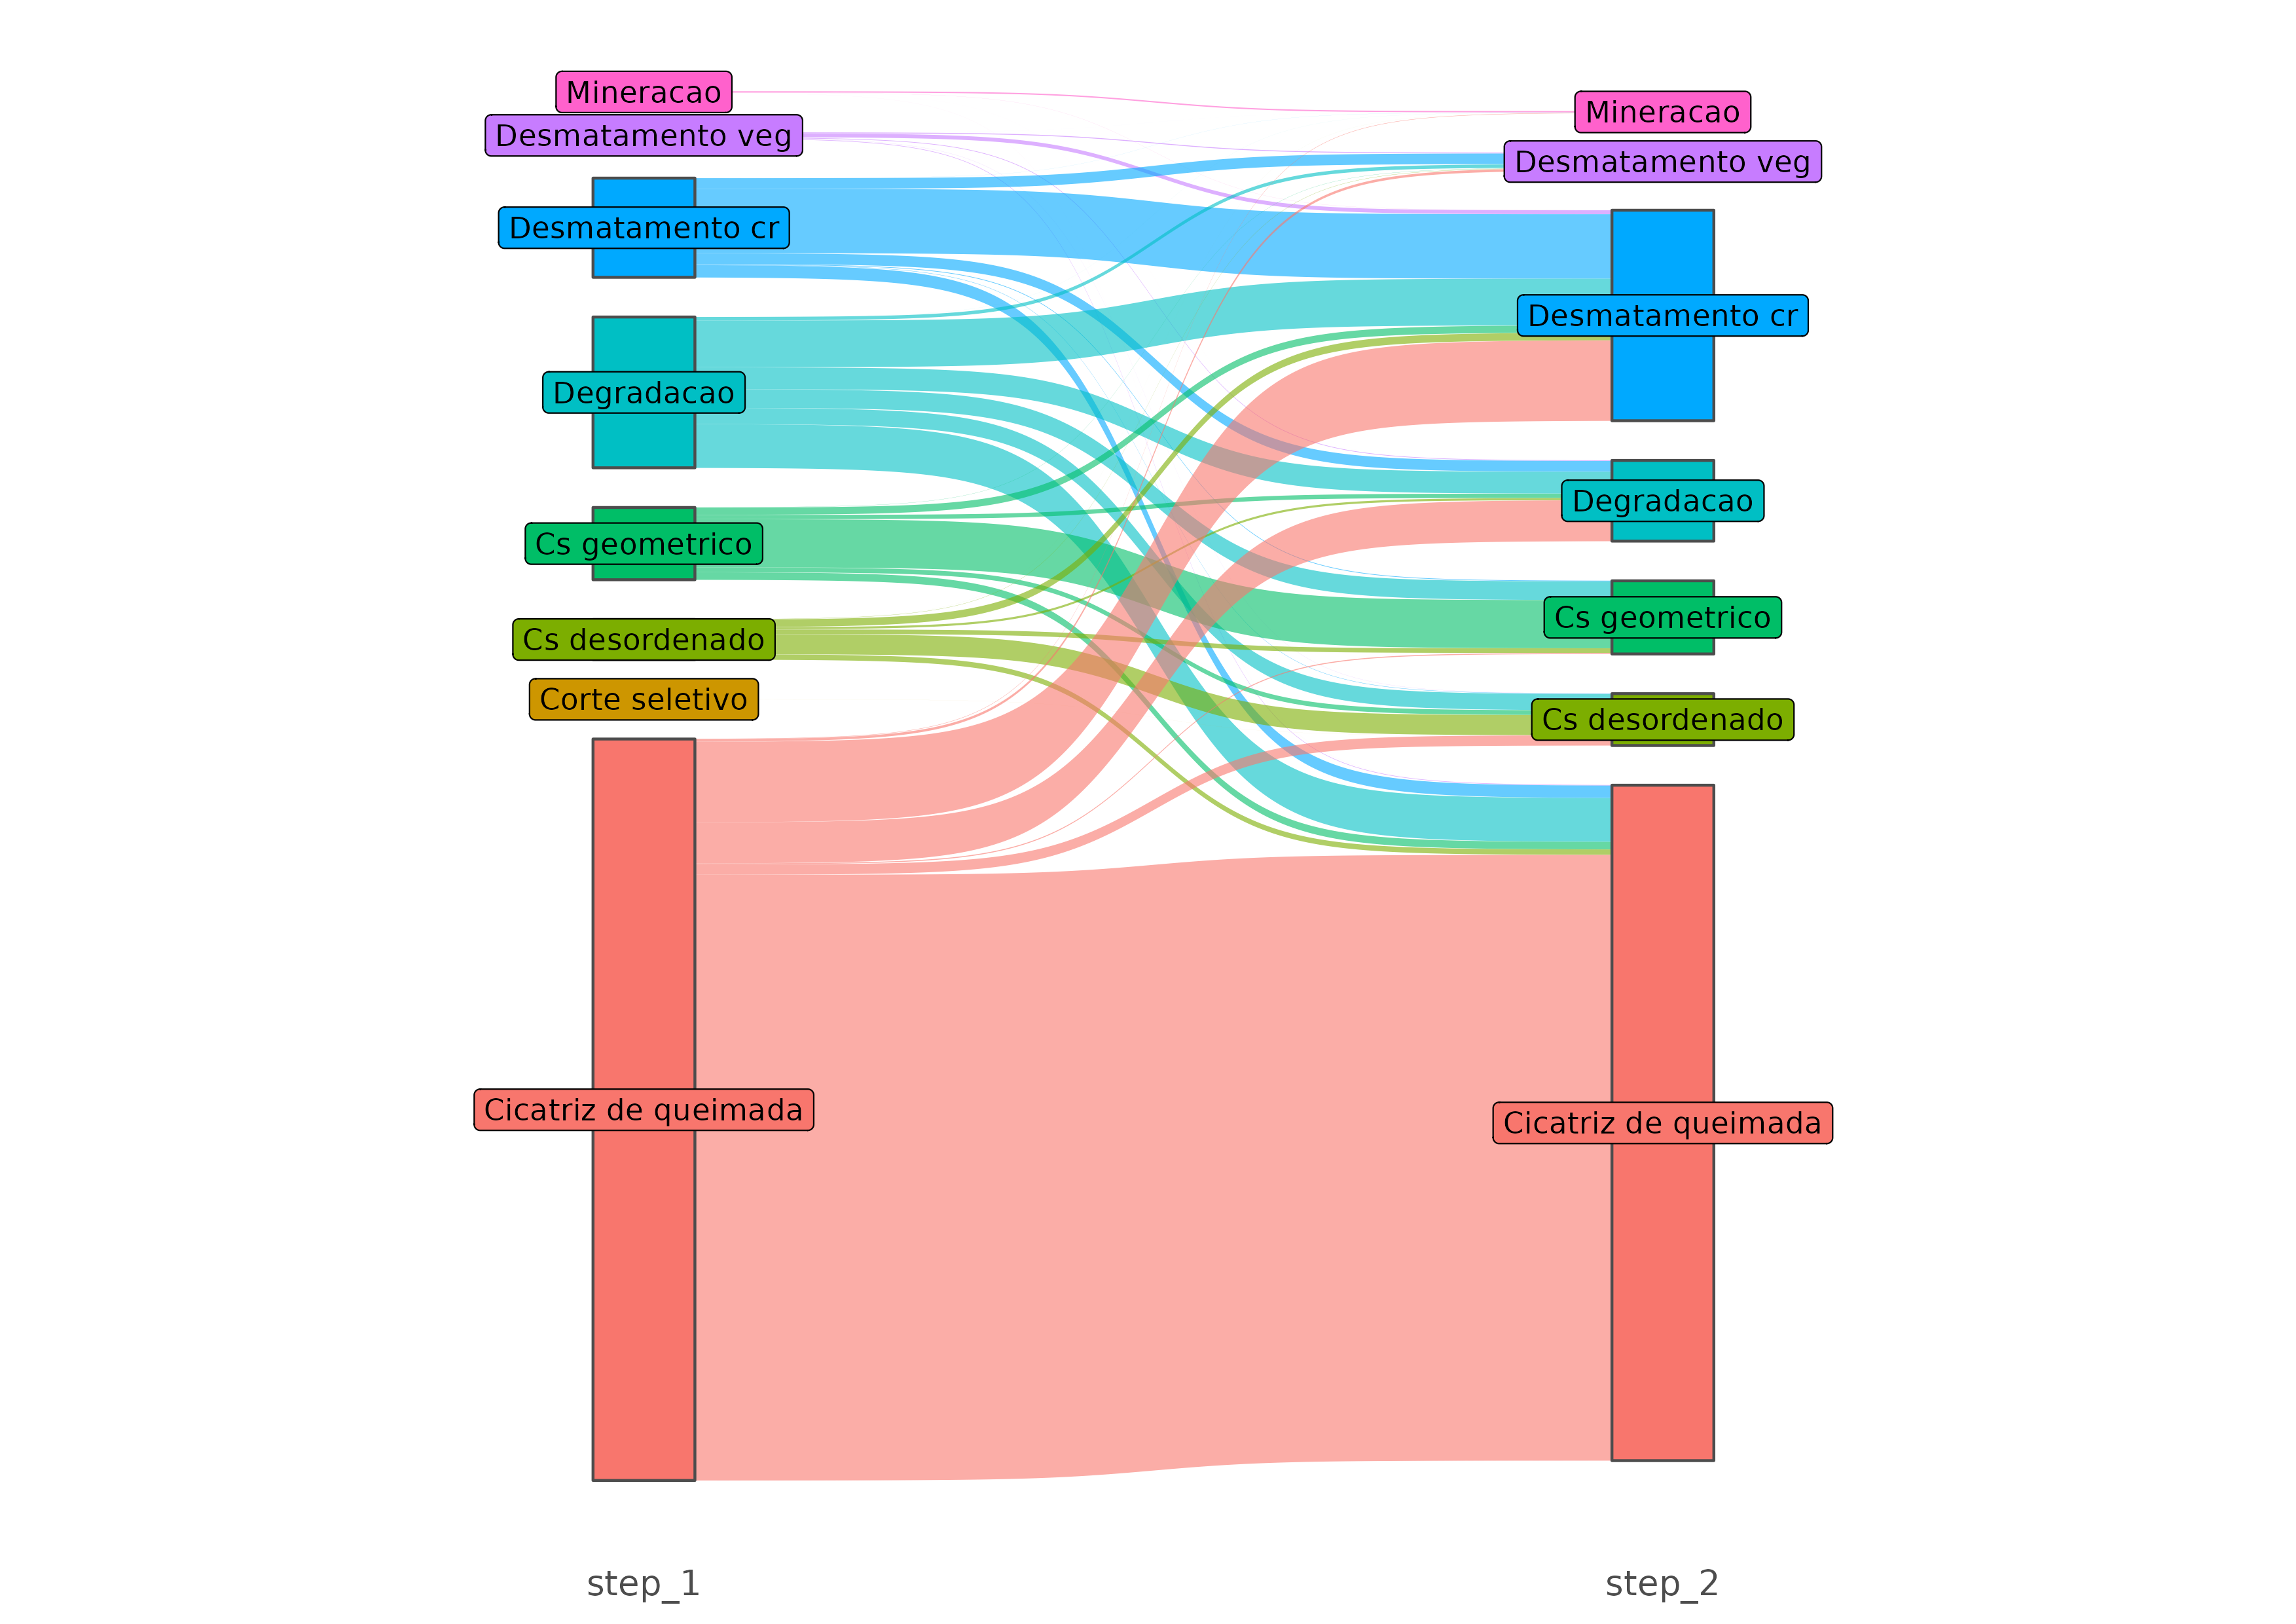
\includegraphics[width=0.65\linewidth]
        {./figures/plot_deter_subarea_trajectory_2.png}
        \caption{Tajectory of subareas with 2 wanings.}
        \label{fig:deter_subarea_trajectory_2}
    \end{figure}
\end{frame}

\begin{frame}[allowframebreaks]
    \frametitle{DETER - Top 10 trajectories (2 warnings)}
    \begingroup\fontsize{7}{9}\selectfont

\begin{longtabu} to \linewidth {>{\raggedright}X>{\raggedright}X>{\raggedleft}X>{\raggedleft}X}
\toprule
position\_1 & position\_2 & area\_ha & n\_traj\\
\midrule
\cellcolor{gray!6}{Cicatriz de queimada} & \cellcolor{gray!6}{Cicatriz de queimada} & \cellcolor{gray!6}{673806.1} & \cellcolor{gray!6}{15015}\\
\cmidrule{1-4}
Cicatriz de queimada & Desmatamento cr & 89540.6 & 5493\\
\cmidrule{1-4}
\cellcolor{gray!6}{Desmatamento cr} & \cellcolor{gray!6}{Desmatamento cr} & \cellcolor{gray!6}{71670.7} & \cellcolor{gray!6}{7882}\\
\cmidrule{1-4}
Cs geometrico & Cs geometrico & 53594.9 & 623\\
\cmidrule{1-4}
\cellcolor{gray!6}{Degradacao} & \cellcolor{gray!6}{Desmatamento cr} & \cellcolor{gray!6}{52004.1} & \cellcolor{gray!6}{3935}\\
\cmidrule{1-4}
Degradacao & Cicatriz de queimada & 48710.2 & 1840\\
\cmidrule{1-4}
\cellcolor{gray!6}{Cicatriz de queimada} & \cellcolor{gray!6}{Degradacao} & \cellcolor{gray!6}{45634.8} & \cellcolor{gray!6}{1701}\\
\cmidrule{1-4}
Degradacao & Degradacao & 24307.9 & 1142\\
\cmidrule{1-4}
\cellcolor{gray!6}{Cs desordenado} & \cellcolor{gray!6}{Cs desordenado} & \cellcolor{gray!6}{22358.4} & \cellcolor{gray!6}{301}\\
\cmidrule{1-4}
Degradacao & Cs geometrico & 20763.4 & 419\\
\cmidrule{1-4}
\cellcolor{gray!6}{Total} & \cellcolor{gray!6}{-} & \cellcolor{gray!6}{1102390.9} & \cellcolor{gray!6}{38351}\\
\bottomrule
\end{longtabu}
\endgroup{}
\end{frame}

\begin{frame}
    \frametitle{DETER subareas (3 warnings)}
    \begin{figure}[h] 
        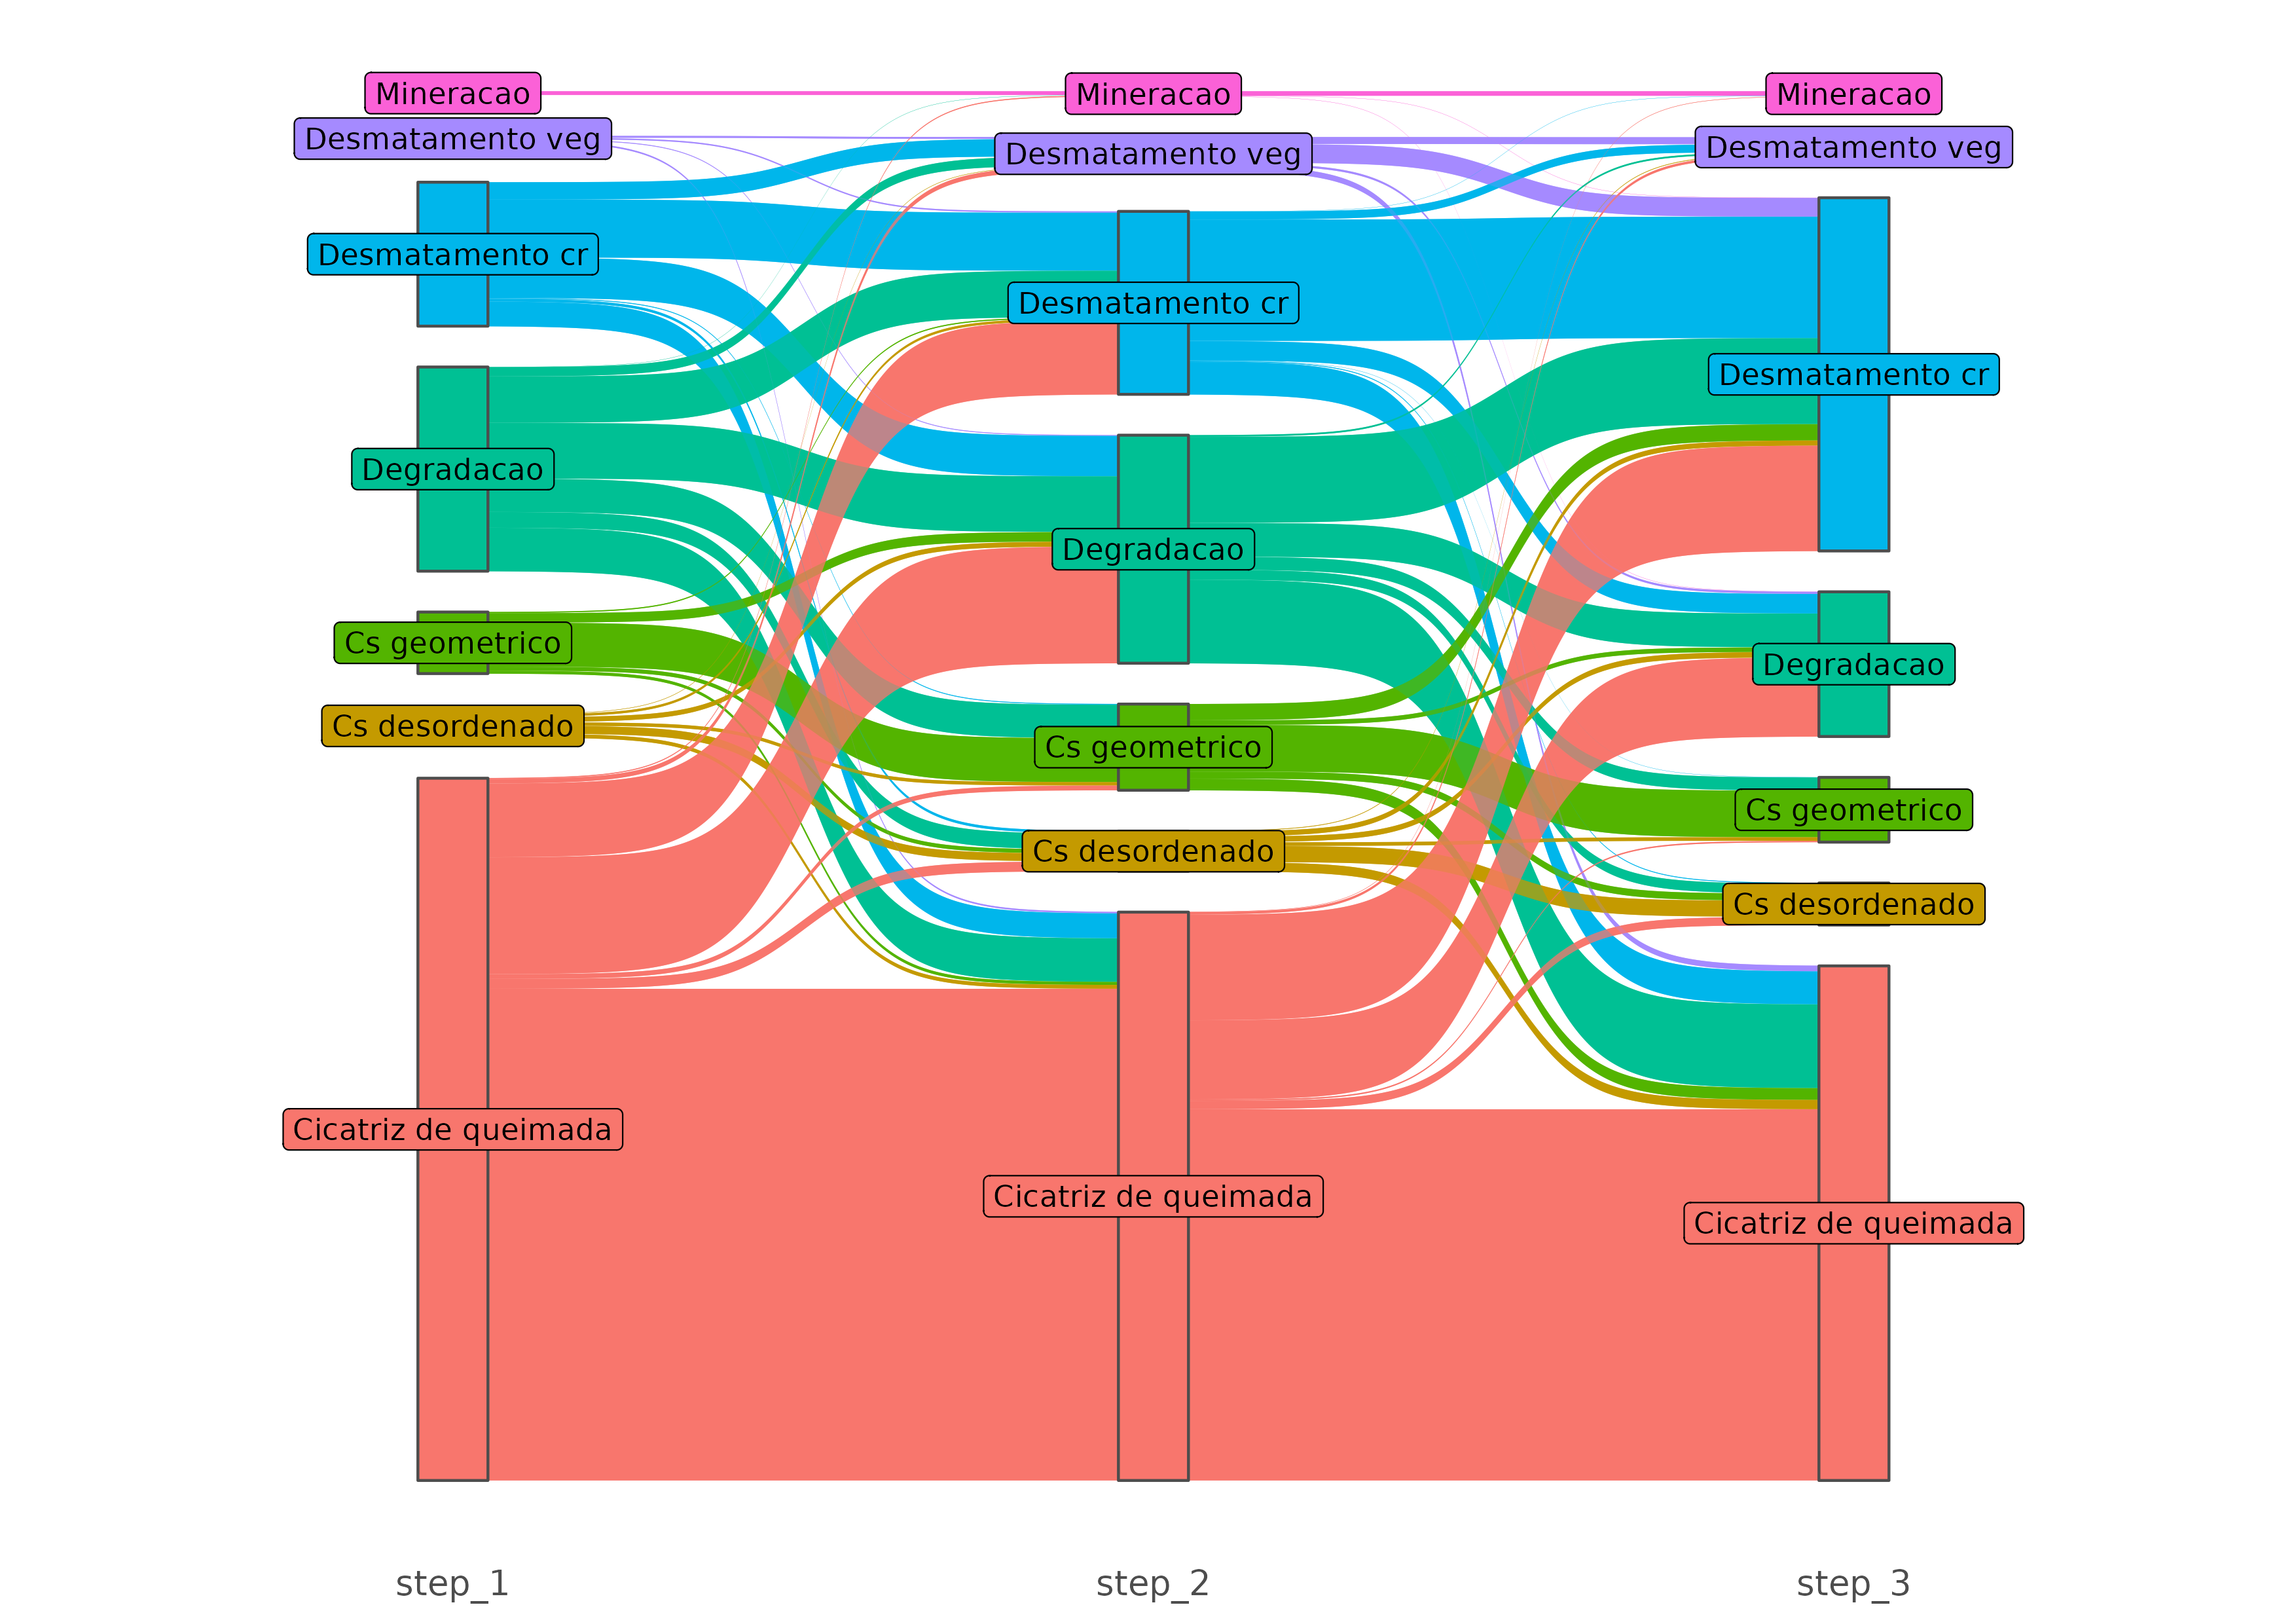
\includegraphics[width=0.65\linewidth]
        {./figures/plot_deter_subarea_trajectory_3.png}
        \caption{Tajectory of subareas with 3 wanings.}
        \label{fig:deter_subarea_trajectory_3}
    \end{figure}
\end{frame}

\begin{frame}[allowframebreaks]
    \frametitle{DETER - Top 10 trajectories (3 warnings)}
    \begingroup\fontsize{7}{9}\selectfont

\begin{longtabu} to \linewidth {>{\raggedright}X>{\raggedright}X>{\raggedright}X>{\raggedleft}X>{\raggedleft}X}
\toprule
position\_1 & position\_2 & position\_3 & area\_ha & n\_traj\\
\midrule
\cellcolor{gray!6}{Cicatriz de queimada} & \cellcolor{gray!6}{Cicatriz de queimada} & \cellcolor{gray!6}{Cicatriz de queimada} & \cellcolor{gray!6}{96013.6} & \cellcolor{gray!6}{1789}\\
\cmidrule{1-5}
Cicatriz de queimada & Cicatriz de queimada & Degradacao & 11700.9 & 345\\
\cmidrule{1-5}
\cellcolor{gray!6}{Cicatriz de queimada} & \cellcolor{gray!6}{Degradacao} & \cellcolor{gray!6}{Cicatriz de queimada} & \cellcolor{gray!6}{11374.3} & \cellcolor{gray!6}{336}\\
\cmidrule{1-5}
Cs geometrico & Cs geometrico & Cs geometrico & 10345.3 & 145\\
\cmidrule{1-5}
\cellcolor{gray!6}{Cicatriz de queimada} & \cellcolor{gray!6}{Cicatriz de queimada} & \cellcolor{gray!6}{Desmatamento cr} & \cellcolor{gray!6}{8944.6} & \cellcolor{gray!6}{423}\\
\cmidrule{1-5}
Degradacao & Cs geometrico & Cs geometrico & 3016.7 & 82\\
\cmidrule{1-5}
\cellcolor{gray!6}{Cicatriz de queimada} & \cellcolor{gray!6}{Degradacao} & \cellcolor{gray!6}{Degradacao} & \cellcolor{gray!6}{2481.7} & \cellcolor{gray!6}{92}\\
\cmidrule{1-5}
Cicatriz de queimada & Desmatamento cr & Desmatamento cr & 2474.5 & 196\\
\cmidrule{1-5}
\cellcolor{gray!6}{Cicatriz de queimada} & \cellcolor{gray!6}{Degradacao} & \cellcolor{gray!6}{Desmatamento cr} & \cellcolor{gray!6}{2353.2} & \cellcolor{gray!6}{173}\\
\cmidrule{1-5}
Cs geometrico & Degradacao & Cs geometrico & 2247.7 & 31\\
\cmidrule{1-5}
\cellcolor{gray!6}{Total} & \cellcolor{gray!6}{-} & \cellcolor{gray!6}{-} & \cellcolor{gray!6}{150952.4} & \cellcolor{gray!6}{3612}\\
\bottomrule
\end{longtabu}
\endgroup{}
\end{frame}

\begin{frame}
    \frametitle{DETER subareas (4 warnings)}
    \begin{figure}[h] 
        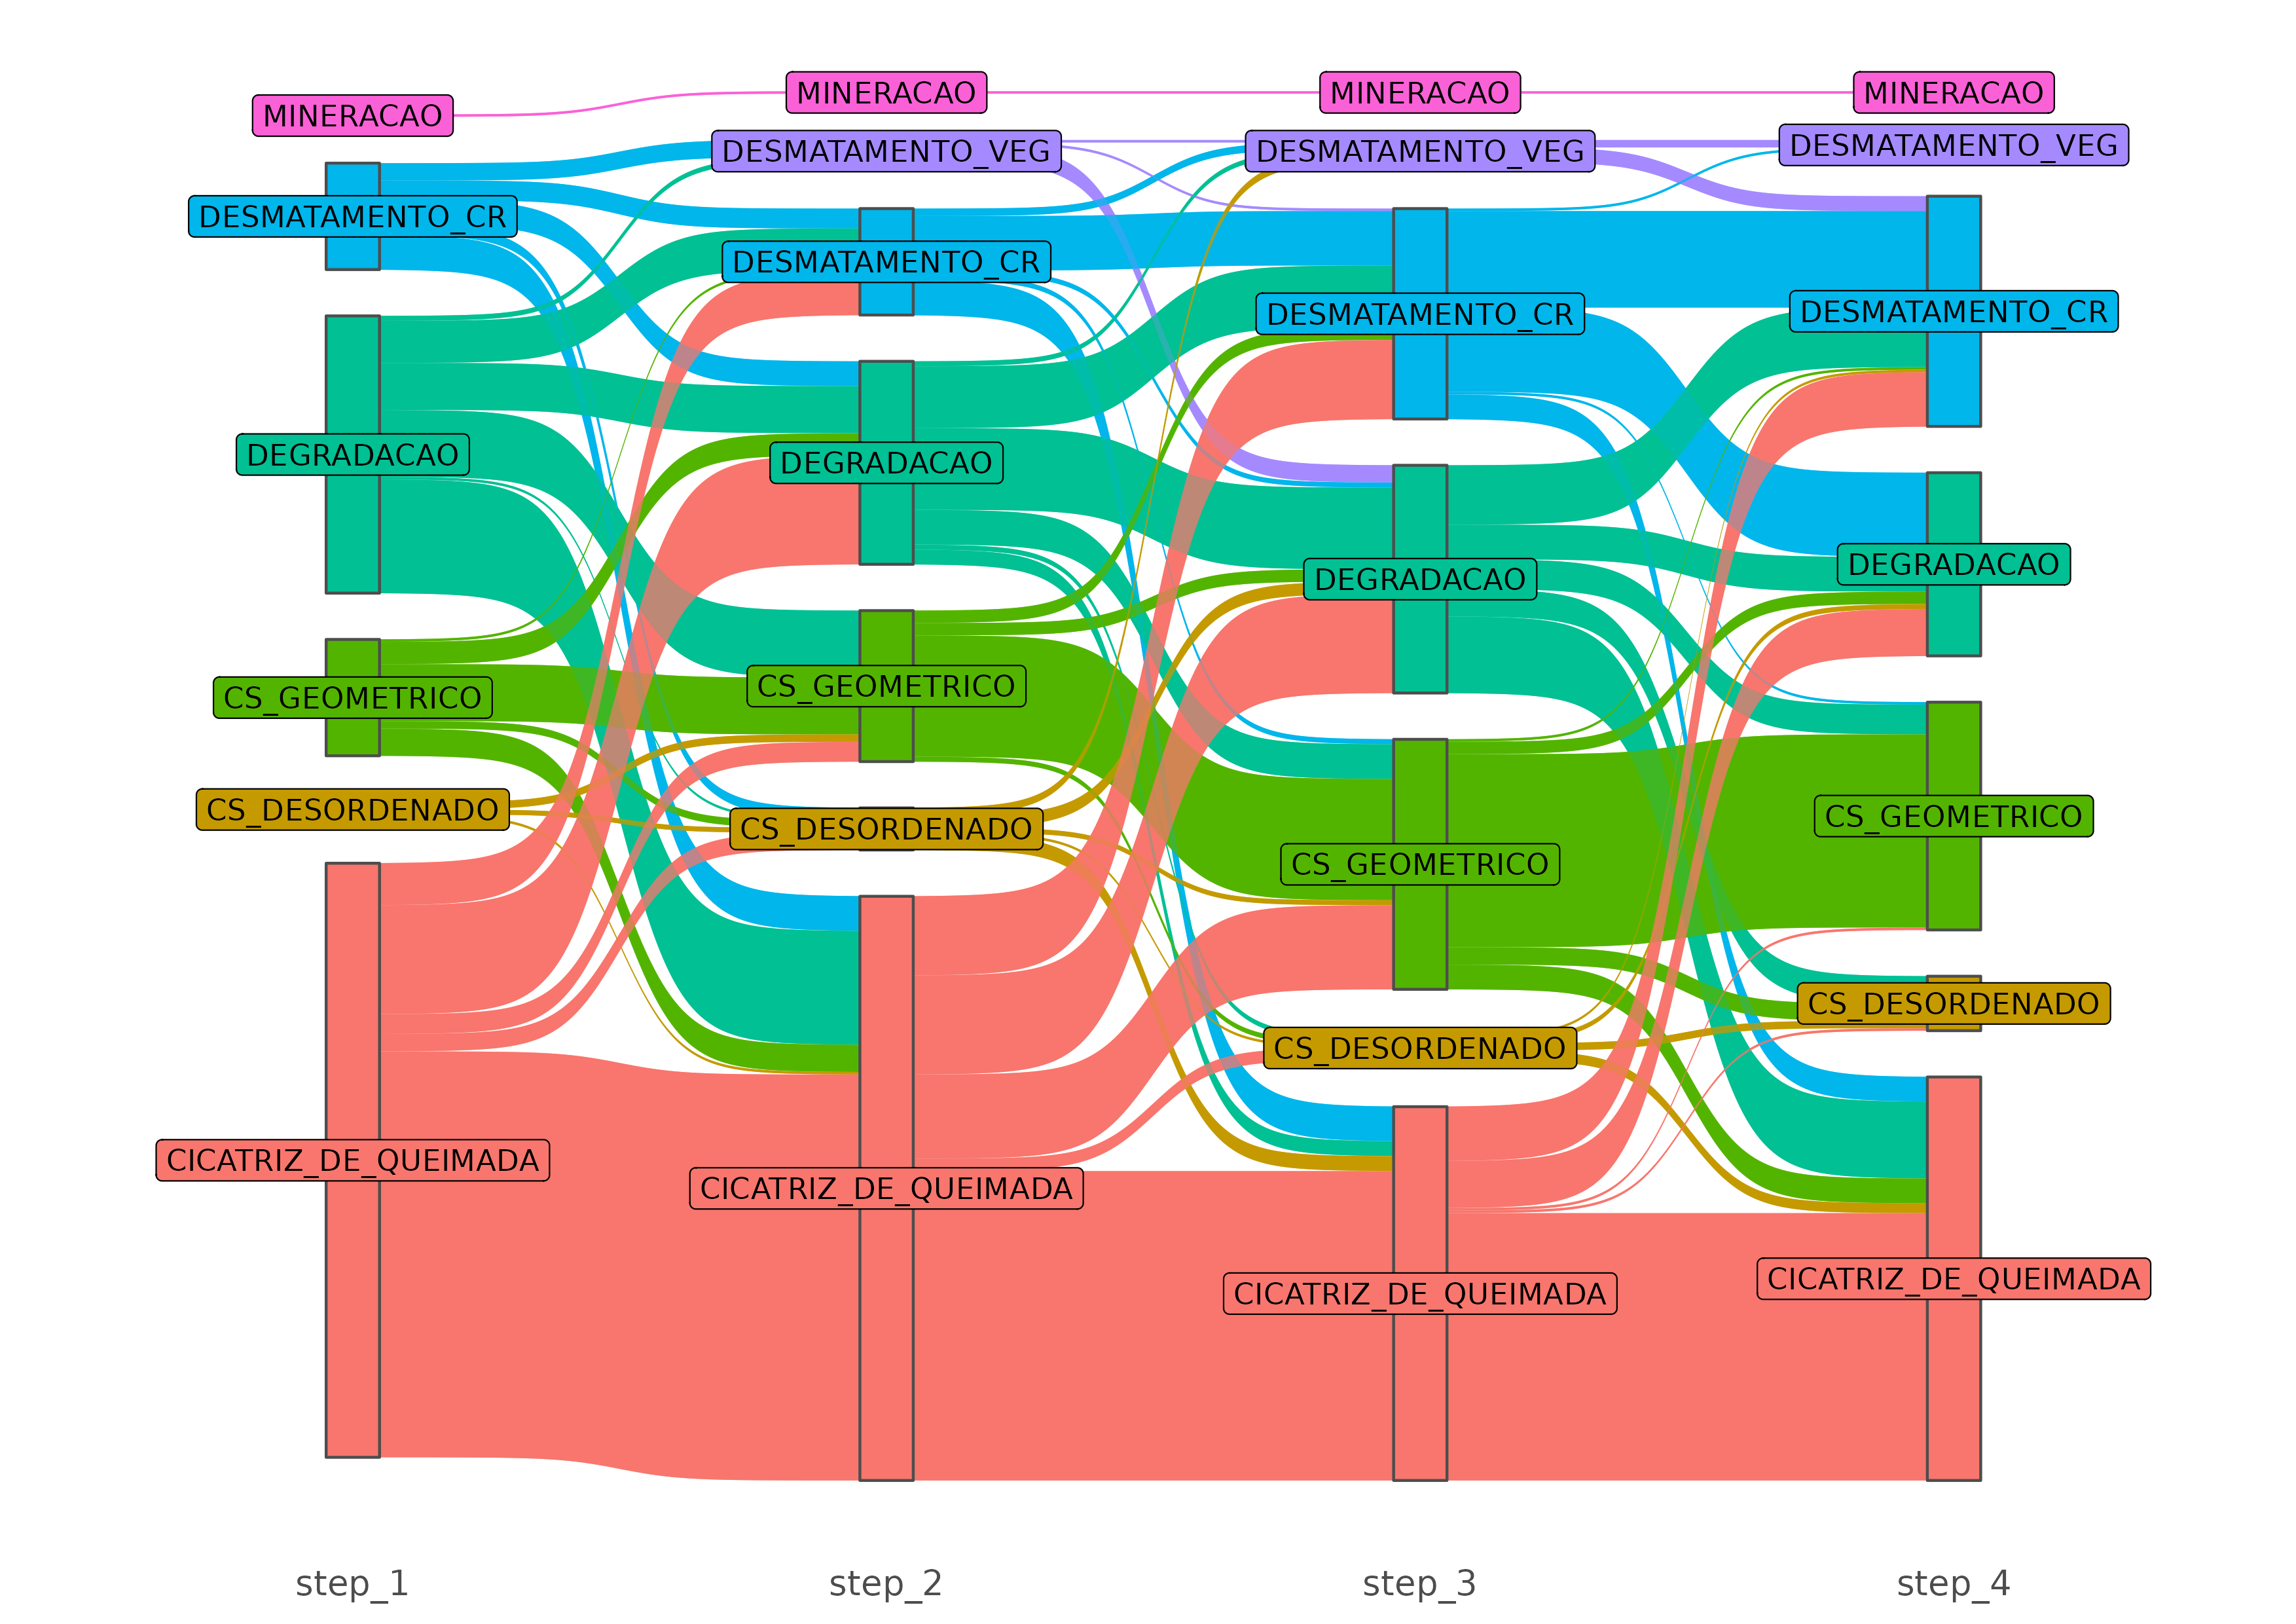
\includegraphics[width=0.65\linewidth]
        {./figures/plot_deter_subarea_trajectory_4.png}
        \caption{Tajectory of subareas with 4 wanings.}
        \label{fig:deter_subarea_trajectory_4}
    \end{figure}
\end{frame}

\begin{frame}[allowframebreaks]
    \frametitle{DETER - Top 10 trajectories (4 warnings)}
    \begingroup\fontsize{7}{9}\selectfont

\begin{longtabu} to \linewidth {>{\raggedright}X>{\raggedright}X>{\raggedright}X>{\raggedright}X>{\raggedleft}X>{\raggedleft}X}
\toprule
position\_1 & position\_2 & position\_3 & position\_4 & area\_ha & n\_traj\\
\midrule
\cellcolor{gray!6}{Cicatriz de queimada} & \cellcolor{gray!6}{Cicatriz de queimada} & \cellcolor{gray!6}{Cicatriz de queimada} & \cellcolor{gray!6}{Cicatriz de queimada} & \cellcolor{gray!6}{3003.6} & \cellcolor{gray!6}{92}\\
\cmidrule{1-6}
Cs geometrico & Cs geometrico & Cs geometrico & Cs geometrico & 892.2 & 16\\
\cmidrule{1-6}
\cellcolor{gray!6}{Cicatriz de queimada} & \cellcolor{gray!6}{Cicatriz de queimada} & \cellcolor{gray!6}{Cicatriz de queimada} & \cellcolor{gray!6}{Degradacao} & \cellcolor{gray!6}{725.4} & \cellcolor{gray!6}{12}\\
\cmidrule{1-6}
Cicatriz de queimada & Cicatriz de queimada & Desmatamento cr & Degradacao & 525.2 & 10\\
\cmidrule{1-6}
\cellcolor{gray!6}{Degradacao} & \cellcolor{gray!6}{Cs geometrico} & \cellcolor{gray!6}{Cs geometrico} & \cellcolor{gray!6}{Cs geometrico} & \cellcolor{gray!6}{515.6} & \cellcolor{gray!6}{16}\\
\cmidrule{1-6}
Cicatriz de queimada & Cicatriz de queimada & Degradacao & Desmatamento cr & 466.3 & 8\\
\cmidrule{1-6}
\cellcolor{gray!6}{Cicatriz de queimada} & \cellcolor{gray!6}{Degradacao} & \cellcolor{gray!6}{Degradacao} & \cellcolor{gray!6}{Cicatriz de queimada} & \cellcolor{gray!6}{431.0} & \cellcolor{gray!6}{21}\\
\cmidrule{1-6}
Cicatriz de queimada & Desmatamento cr & Cicatriz de queimada & Cicatriz de queimada & 390.8 & 9\\
\cmidrule{1-6}
\cellcolor{gray!6}{Degradacao} & \cellcolor{gray!6}{Cs geometrico} & \cellcolor{gray!6}{Cs geometrico} & \cellcolor{gray!6}{Cicatriz de queimada} & \cellcolor{gray!6}{387.4} & \cellcolor{gray!6}{7}\\
\cmidrule{1-6}
Degradacao & Cicatriz de queimada & Cs geometrico & Cs geometrico & 373.2 & 23\\
\cmidrule{1-6}
\cellcolor{gray!6}{Total} & \cellcolor{gray!6}{-} & \cellcolor{gray!6}{-} & \cellcolor{gray!6}{-} & \cellcolor{gray!6}{7710.8} & \cellcolor{gray!6}{214}\\
\bottomrule
\end{longtabu}
\endgroup{}
\end{frame}

\begin{frame}
    \frametitle{DETER subareas (5 warnings)}
    \begin{figure}[h] 
        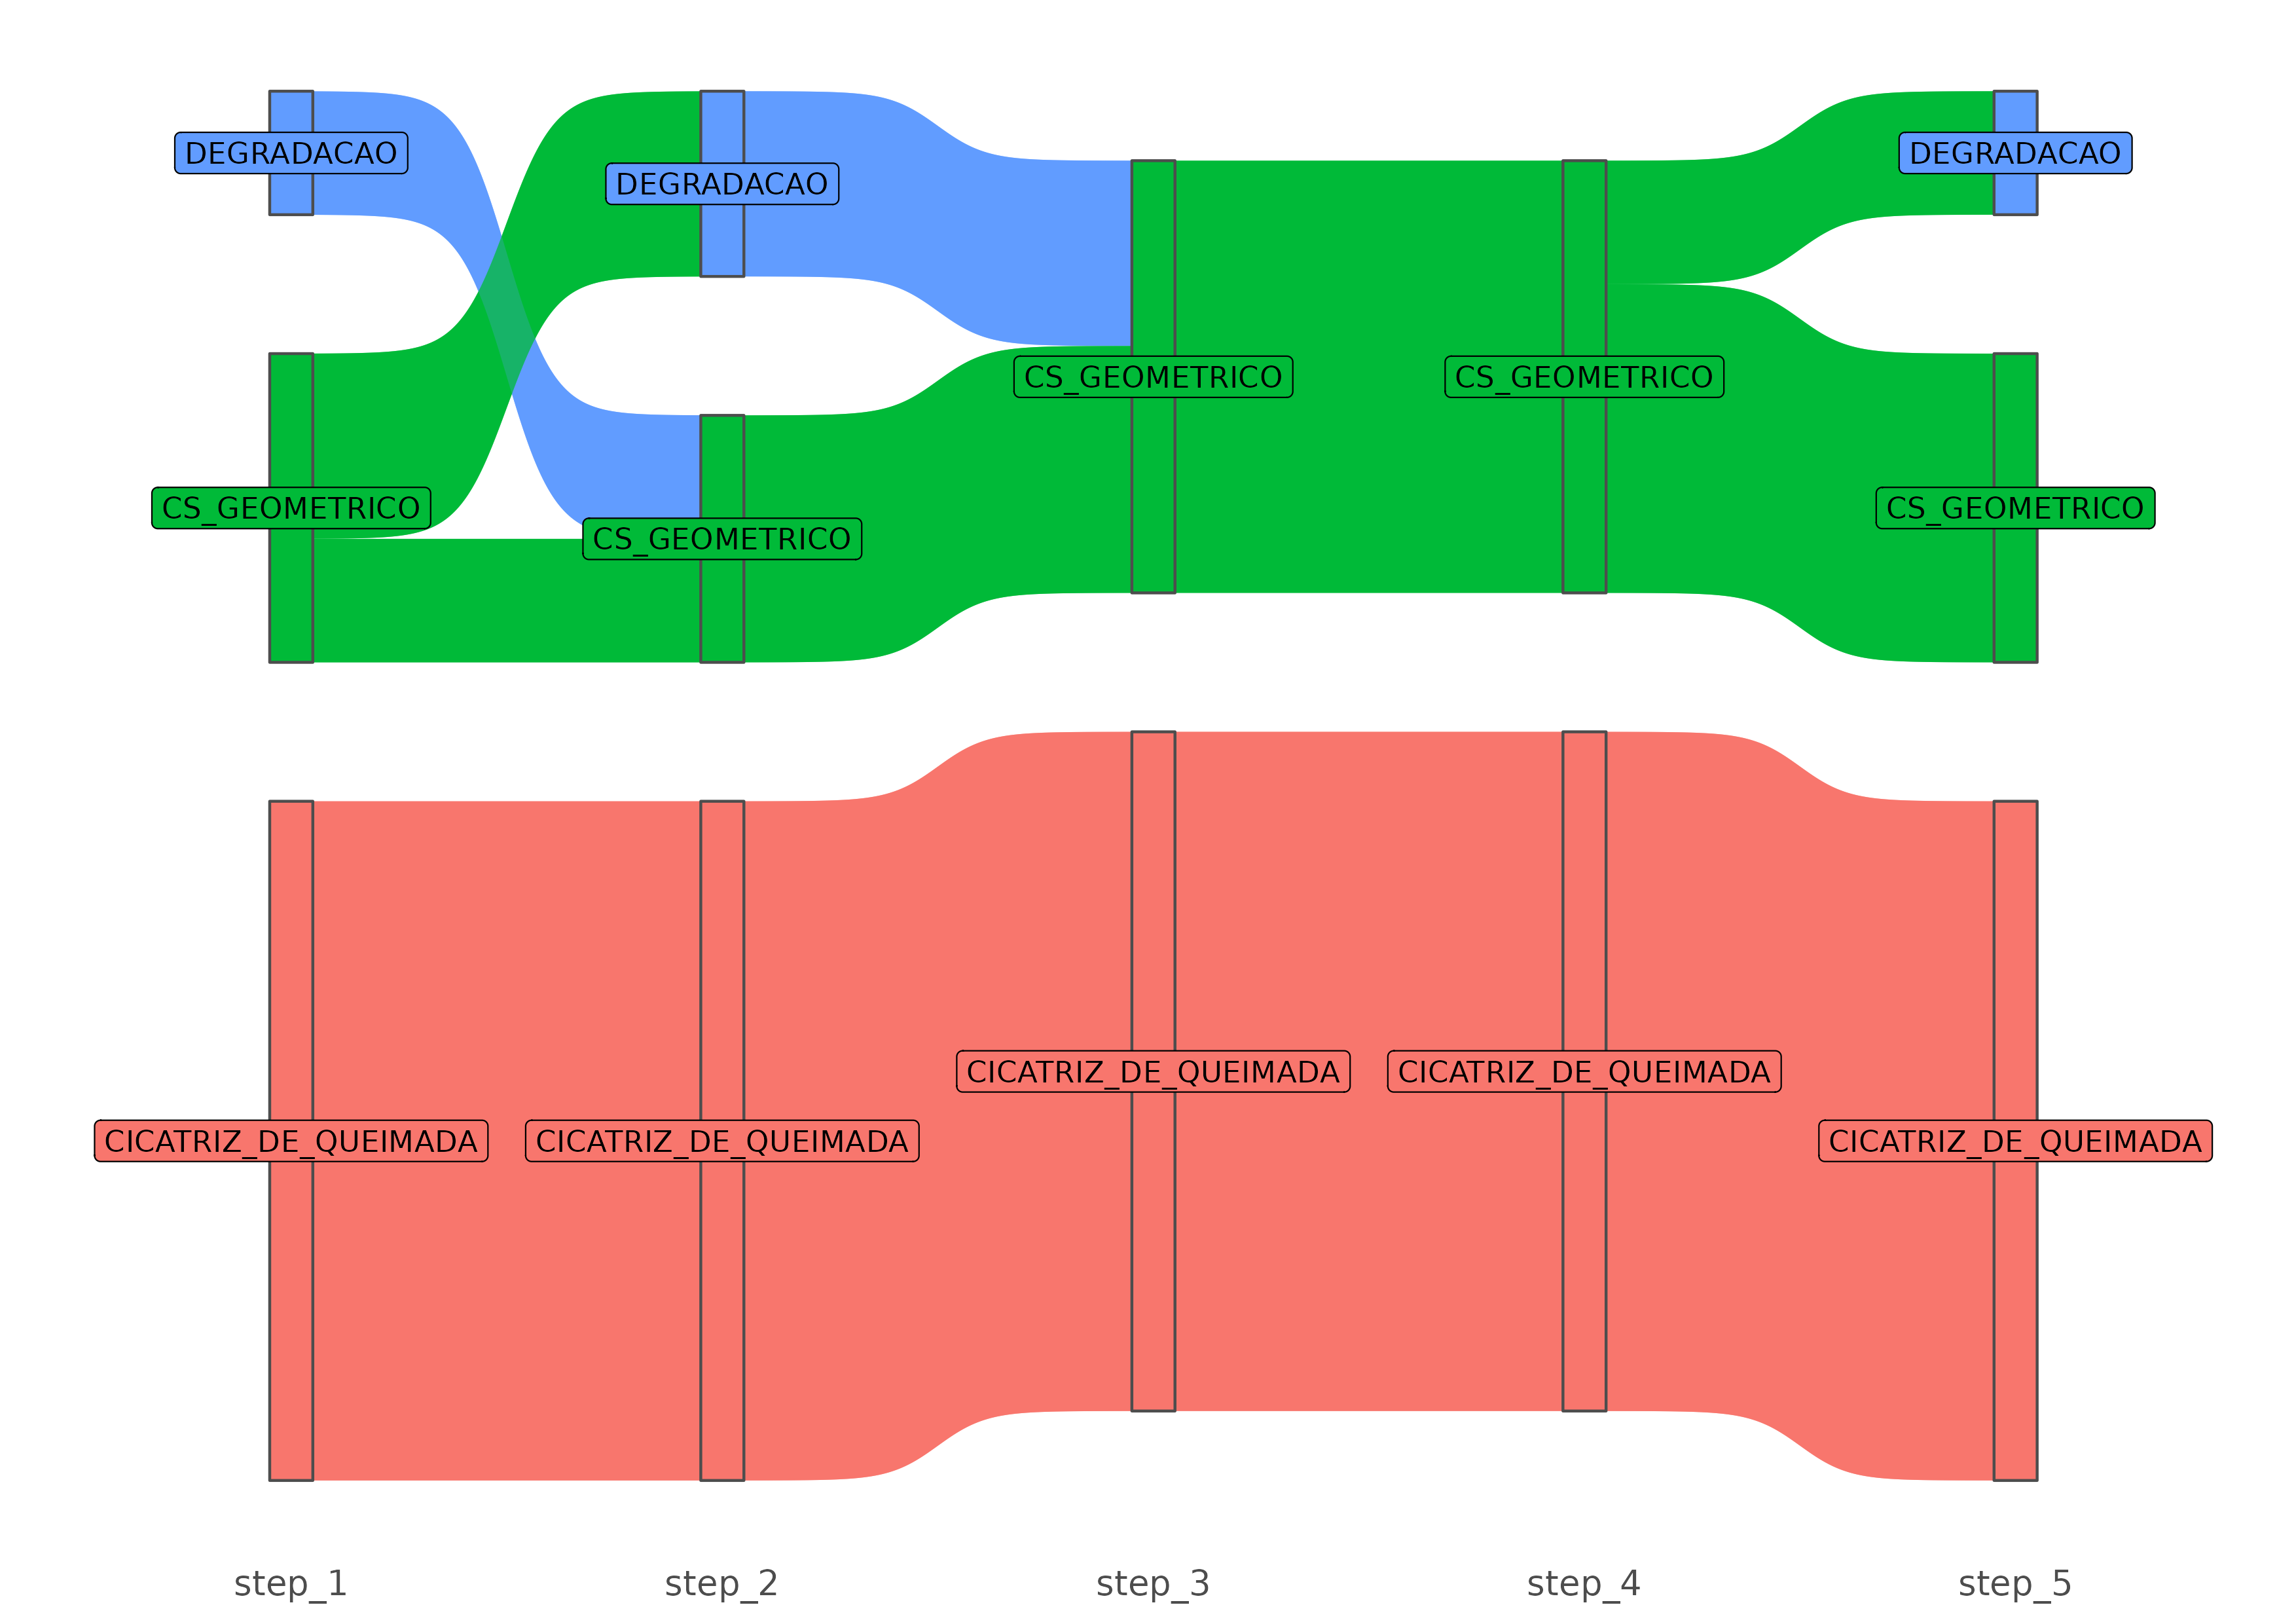
\includegraphics[width=0.65\linewidth]
        {./figures/plot_deter_subarea_trajectory_5.png}
        \caption{Tajectory of subareas with 5 wanings.}
        \label{fig:deter_subarea_trajectory_5}
    \end{figure}
\end{frame}

\begin{frame}[allowframebreaks]
    \frametitle{DETER - Top 10 trajectories (5 warnings)}
    \begingroup\fontsize{7}{9}\selectfont

\begin{longtabu} to \linewidth {>{\raggedright}X>{\raggedright}X>{\raggedright}X>{\raggedright}X>{\raggedleft}X>{\raggedleft}X}
\toprule
position\_1 & position\_2 & position\_3 & position\_4 & area\_ha & n\_traj\\
\midrule
\cellcolor{gray!6}{Cicatriz de queimada} & \cellcolor{gray!6}{Cicatriz de queimada} & \cellcolor{gray!6}{Cicatriz de queimada} & \cellcolor{gray!6}{Cicatriz de queimada} & \cellcolor{gray!6}{3003.6} & \cellcolor{gray!6}{92}\\
\cmidrule{1-6}
Cs geometrico & Cs geometrico & Cs geometrico & Cs geometrico & 892.2 & 16\\
\cmidrule{1-6}
\cellcolor{gray!6}{Cicatriz de queimada} & \cellcolor{gray!6}{Cicatriz de queimada} & \cellcolor{gray!6}{Cicatriz de queimada} & \cellcolor{gray!6}{Degradacao} & \cellcolor{gray!6}{725.4} & \cellcolor{gray!6}{12}\\
\cmidrule{1-6}
Cicatriz de queimada & Cicatriz de queimada & Desmatamento cr & Degradacao & 525.2 & 10\\
\cmidrule{1-6}
\cellcolor{gray!6}{Degradacao} & \cellcolor{gray!6}{Cs geometrico} & \cellcolor{gray!6}{Cs geometrico} & \cellcolor{gray!6}{Cs geometrico} & \cellcolor{gray!6}{515.6} & \cellcolor{gray!6}{16}\\
\cmidrule{1-6}
Cicatriz de queimada & Cicatriz de queimada & Degradacao & Desmatamento cr & 466.3 & 8\\
\cmidrule{1-6}
\cellcolor{gray!6}{Cicatriz de queimada} & \cellcolor{gray!6}{Degradacao} & \cellcolor{gray!6}{Degradacao} & \cellcolor{gray!6}{Cicatriz de queimada} & \cellcolor{gray!6}{431.0} & \cellcolor{gray!6}{21}\\
\cmidrule{1-6}
Cicatriz de queimada & Desmatamento cr & Cicatriz de queimada & Cicatriz de queimada & 390.8 & 9\\
\cmidrule{1-6}
\cellcolor{gray!6}{Degradacao} & \cellcolor{gray!6}{Cs geometrico} & \cellcolor{gray!6}{Cs geometrico} & \cellcolor{gray!6}{Cicatriz de queimada} & \cellcolor{gray!6}{387.4} & \cellcolor{gray!6}{7}\\
\cmidrule{1-6}
Degradacao & Cicatriz de queimada & Cs geometrico & Cs geometrico & 373.2 & 23\\
\cmidrule{1-6}
\cellcolor{gray!6}{Total} & \cellcolor{gray!6}{-} & \cellcolor{gray!6}{-} & \cellcolor{gray!6}{-} & \cellcolor{gray!6}{7710.8} & \cellcolor{gray!6}{214}\\
\bottomrule
\end{longtabu}
\endgroup{}
\end{frame}



\subsection{Trajectories (DETER \& PRODES)} 

\begin{frame}
    \frametitle{DETER \& PRODES - Top 10 trajectories (2 warnings)}
    \begin{figure}[h] 
        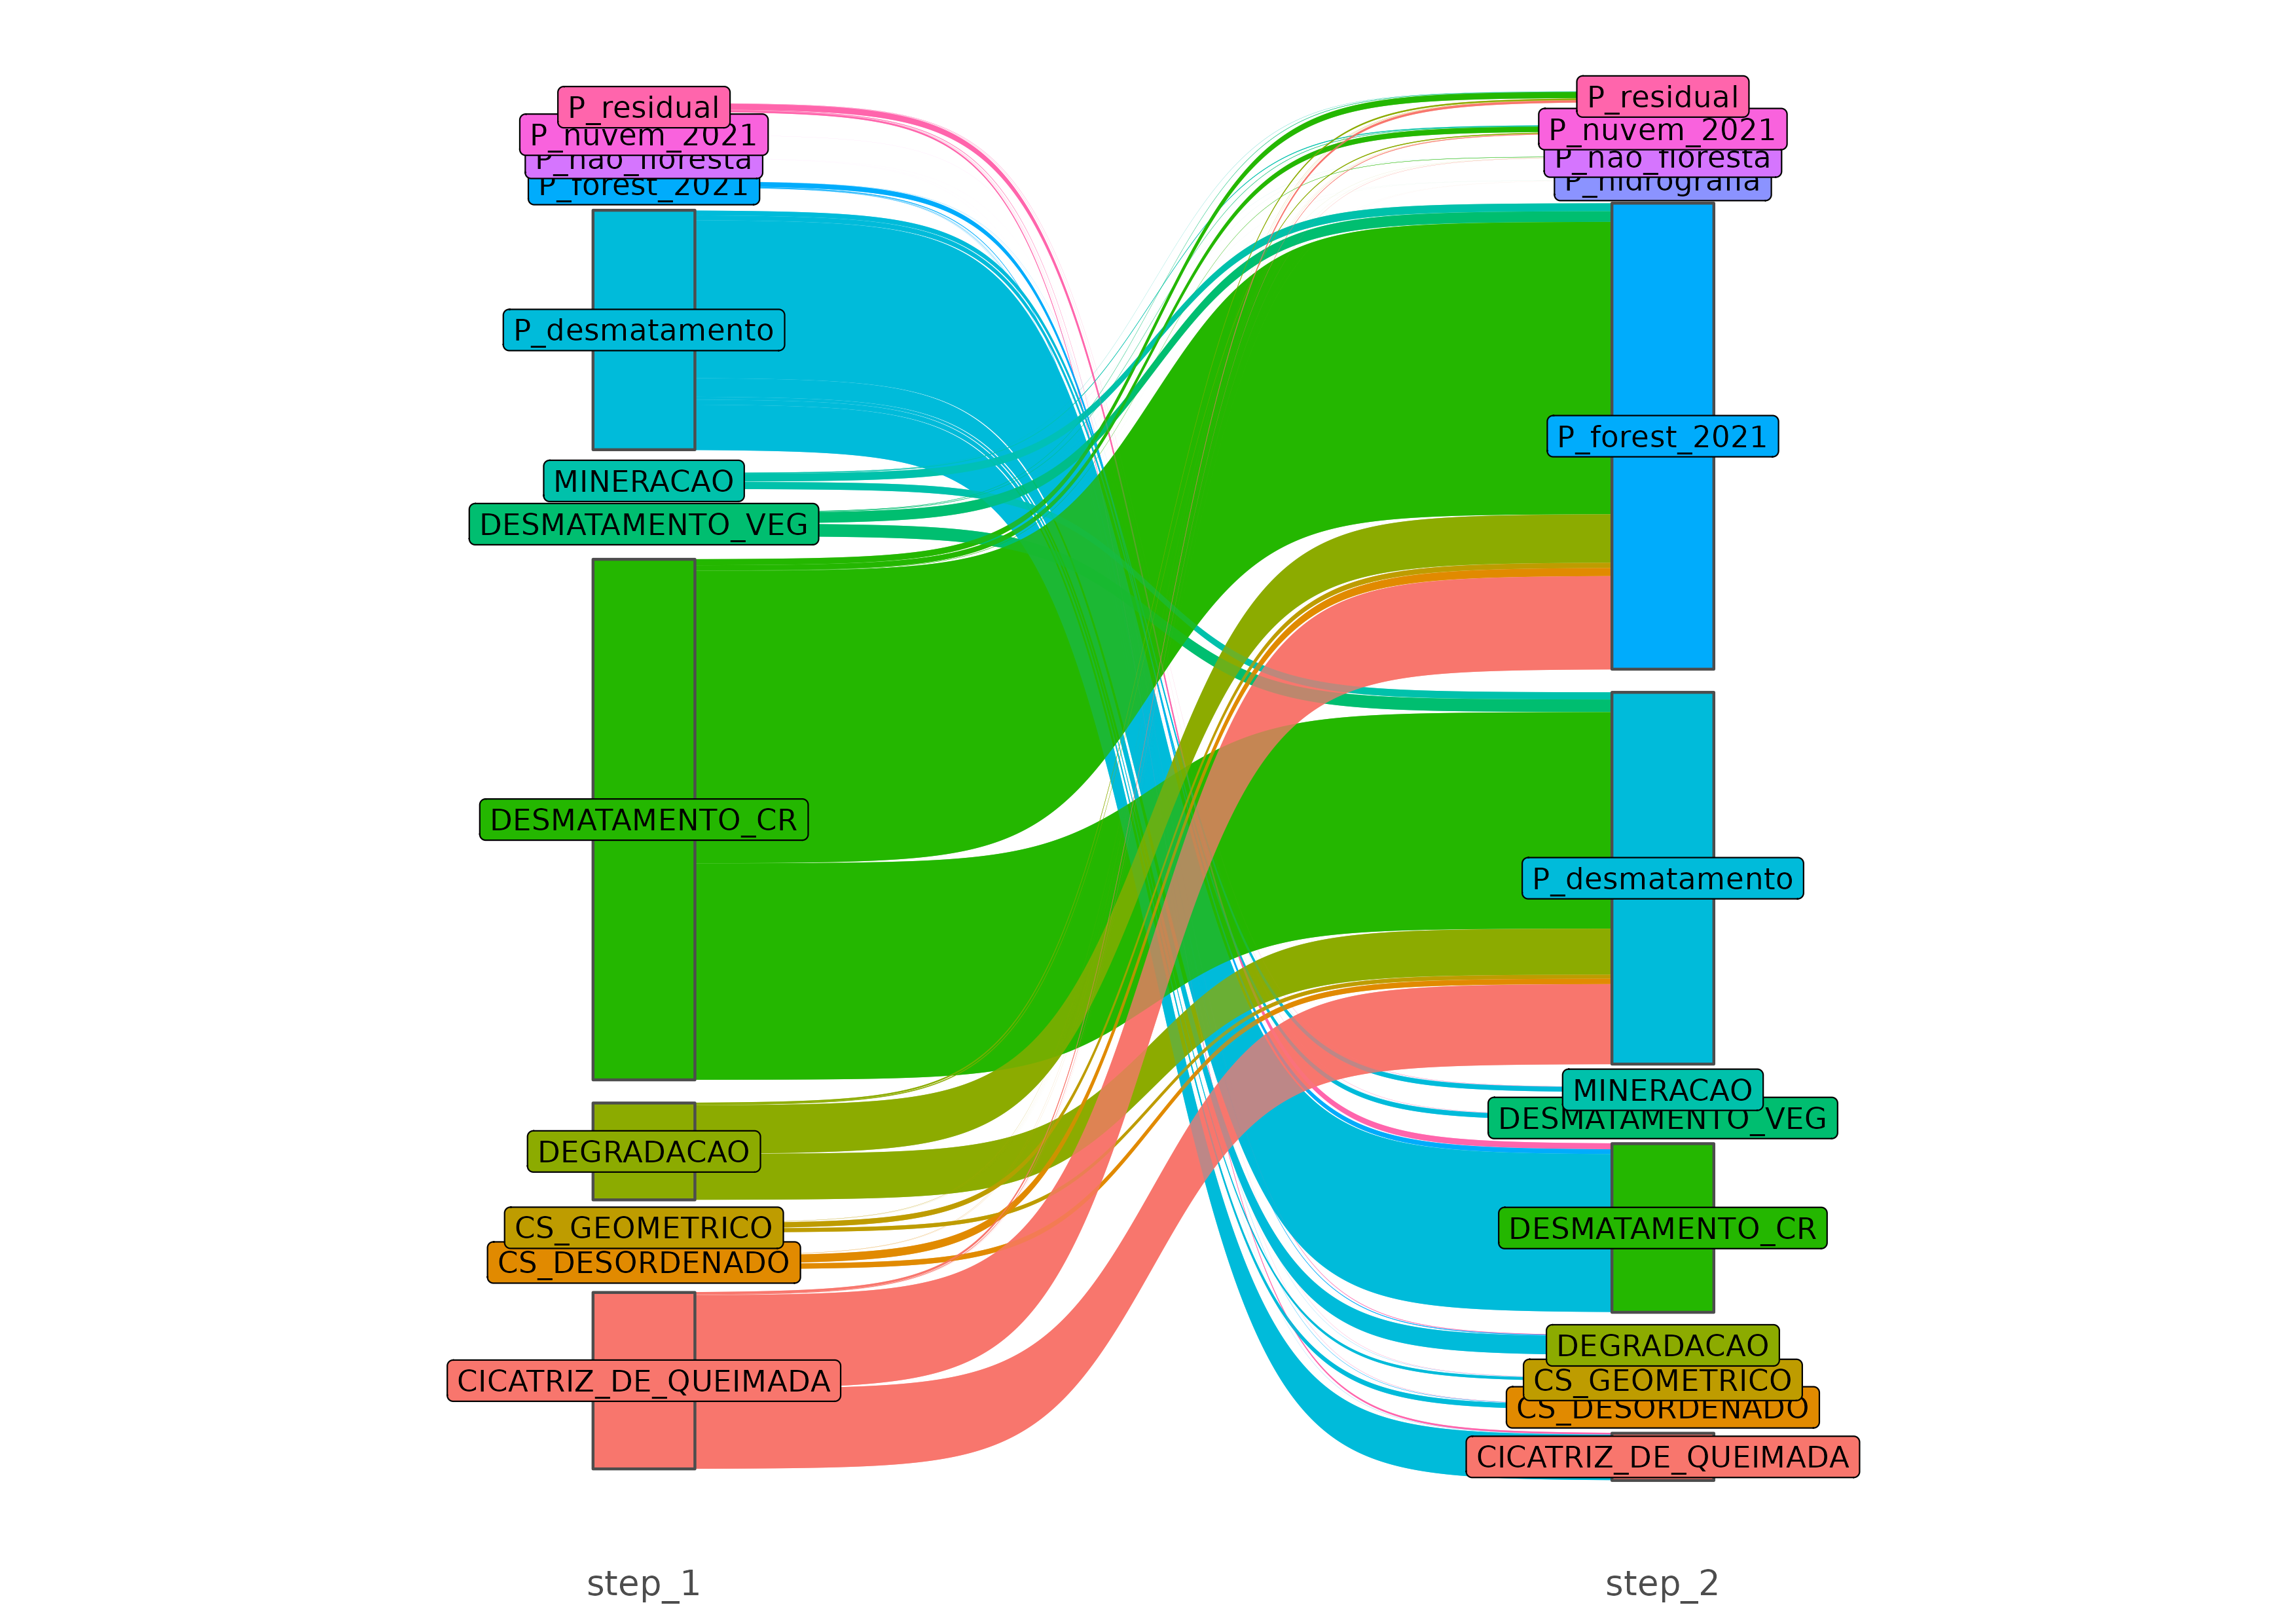
\includegraphics[width=0.65\linewidth]
        {./figures/plot_deter_prodes_subarea_trajectory_2.png}
        \caption{Tajectory of subareas with 2 wanings.}
        \label{fig:deter_prodes_subarea_trajectory_2}
    \end{figure}
\end{frame}

\begin{frame}[allowframebreaks]
    \frametitle{DETER \& PRODES - Top 10 trajectories (2 warnings)}
    \begingroup\fontsize{7}{9}\selectfont

\begin{longtabu} to \linewidth {>{\raggedright}X>{\raggedright}X>{\raggedleft}X>{\raggedleft}X>{\raggedleft}X>{\raggedleft}X}
\toprule
position\_1 & position\_2 & area\_ha & n\_traj & p\_area & p\_traj\\
\midrule
\cellcolor{gray!6}{Cicatriz de queimada} & \cellcolor{gray!6}{P forest} & \cellcolor{gray!6}{1041281.5} & \cellcolor{gray!6}{12645} & \cellcolor{gray!6}{18.8} & \cellcolor{gray!6}{8.4}\\
\cmidrule{1-6}
Cicatriz de queimada & P deforestation & 927627.3 & 10848 & 16.8 & 7.2\\
\cmidrule{1-6}
\cellcolor{gray!6}{Desmatamento cr} & \cellcolor{gray!6}{P forest} & \cellcolor{gray!6}{838982.5} & \cellcolor{gray!6}{39589} & \cellcolor{gray!6}{15.2} & \cellcolor{gray!6}{26.3}\\
\cmidrule{1-6}
Desmatamento cr & P deforestation & 575218.9 & 29323 & 10.4 & 19.5\\
\cmidrule{1-6}
\cellcolor{gray!6}{P deforestation} & \cellcolor{gray!6}{Desmatamento cr} & \cellcolor{gray!6}{386346.7} & \cellcolor{gray!6}{21391} & \cellcolor{gray!6}{7.0} & \cellcolor{gray!6}{14.2}\\
\cmidrule{1-6}
Total & - & 5537714.8 & 150521 & 100.0 & 100.0\\
\bottomrule
\end{longtabu}
\endgroup{}
\end{frame}

\begin{frame}
    \frametitle{DETER \& PRODES subareas (3 warnings)}
    \begin{figure}[h] 
        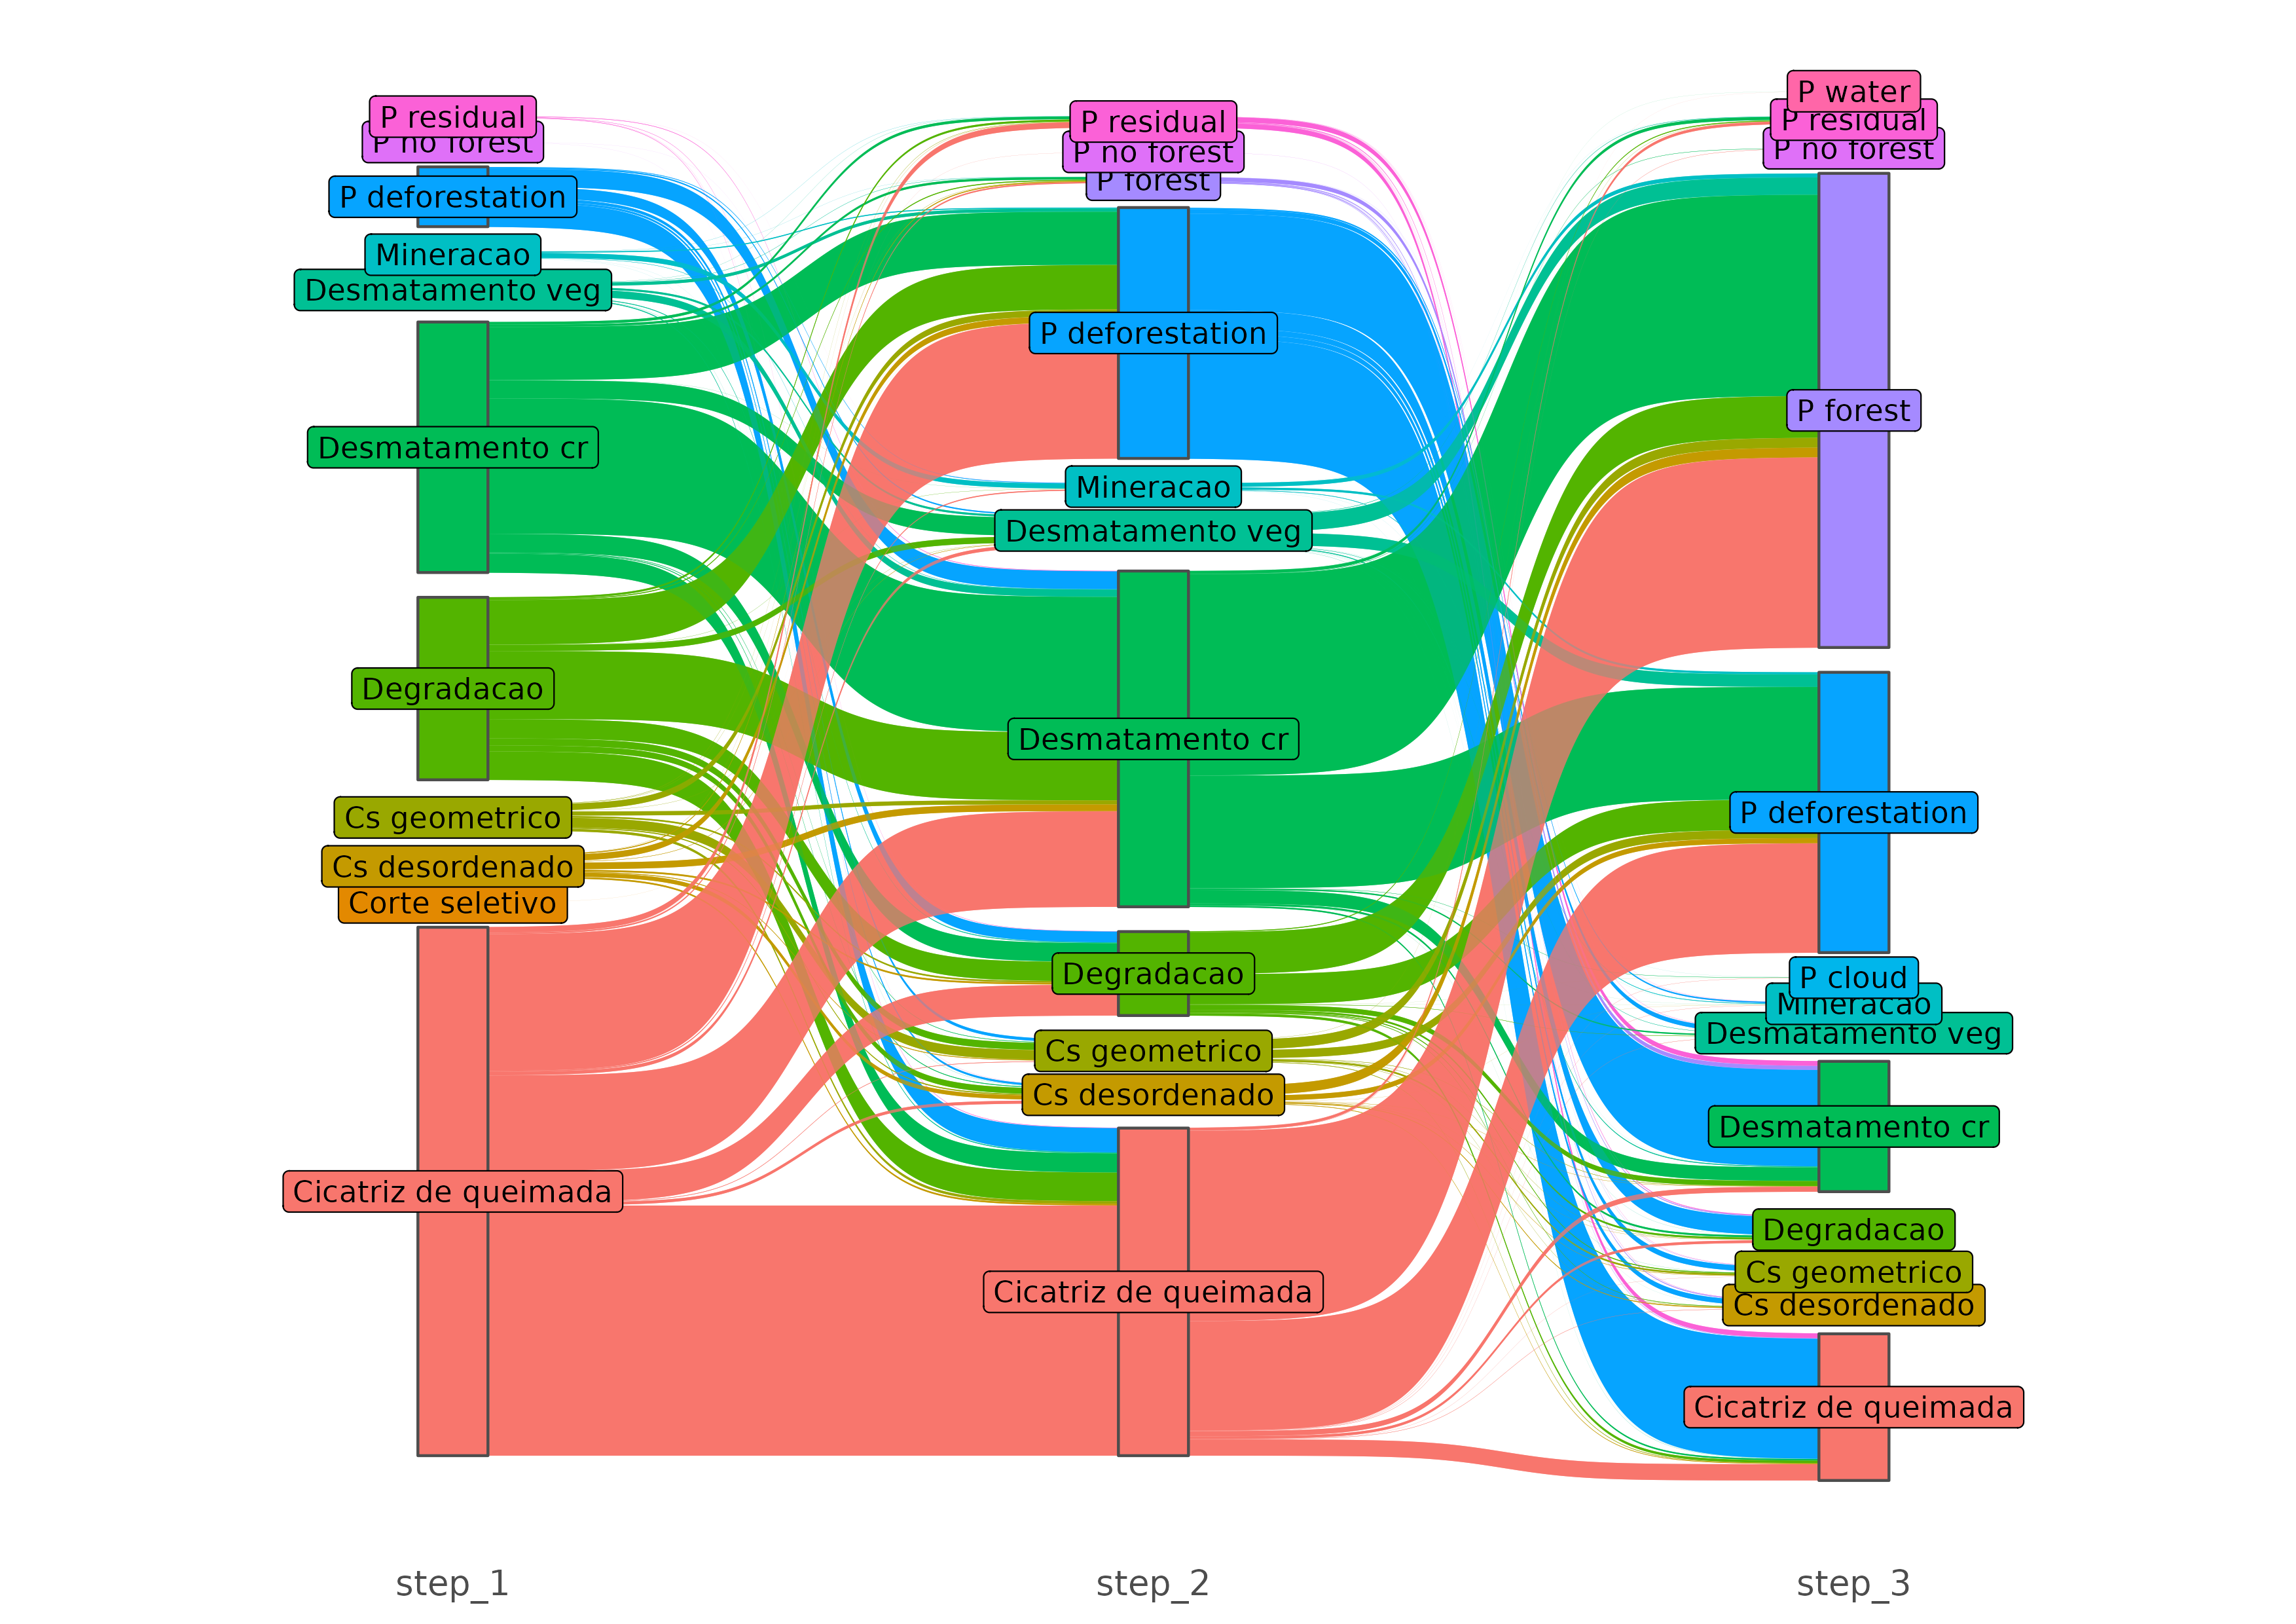
\includegraphics[width=0.65\linewidth]
        {./figures/plot_deter_prodes_subarea_trajectory_3.png}
        \caption{Tajectory of subareas with 3 wanings.}
        \label{fig:deter_prodes_subarea_trajectory_3}
    \end{figure}
\end{frame}

\begin{frame}[allowframebreaks]
    \frametitle{DETER \& PRODES - Top 10 trajectories (3 warnings)}
    \begingroup\fontsize{7}{9}\selectfont

\begin{longtabu} to \linewidth {>{\raggedright}X>{\raggedright}X>{\raggedright}X>{\raggedleft}X>{\raggedleft}X}
\toprule
position\_1 & position\_2 & position\_3 & n\_traj & subarea\_ha\\
\midrule
\cellcolor{gray!6}{Cicatriz de queimada} & \cellcolor{gray!6}{Cicatriz de queimada} & \cellcolor{gray!6}{P desmatamento} & \cellcolor{gray!6}{2836} & \cellcolor{gray!6}{124744.1}\\
\cmidrule{1-5}
Cicatriz de queimada & Cicatriz de queimada & P forest 2021 & 4775 & 227564.0\\
\cmidrule{1-5}
\cellcolor{gray!6}{Cicatriz de queimada} & \cellcolor{gray!6}{Cicatriz de queimada} & \cellcolor{gray!6}{P nao floresta} & \cellcolor{gray!6}{6} & \cellcolor{gray!6}{140.7}\\
\cmidrule{1-5}
Cicatriz de queimada & Cicatriz de queimada & P nuvem 2021 & 3 & 128.9\\
\cmidrule{1-5}
\cellcolor{gray!6}{Cicatriz de queimada} & \cellcolor{gray!6}{Cicatriz de queimada} & \cellcolor{gray!6}{P residual} & \cellcolor{gray!6}{75} & \cellcolor{gray!6}{4048.7}\\
\cmidrule{1-5}
Cicatriz de queimada & Cs desordenado & P desmatamento & 29 & 2354.8\\
\cmidrule{1-5}
\cellcolor{gray!6}{Cicatriz de queimada} & \cellcolor{gray!6}{Cs desordenado} & \cellcolor{gray!6}{P forest 2021} & \cellcolor{gray!6}{63} & \cellcolor{gray!6}{3799.2}\\
\cmidrule{1-5}
Cicatriz de queimada & Cs geometrico & P desmatamento & 11 & 311.1\\
\cmidrule{1-5}
\cellcolor{gray!6}{Cicatriz de queimada} & \cellcolor{gray!6}{Cs geometrico} & \cellcolor{gray!6}{P forest 2021} & \cellcolor{gray!6}{4} & \cellcolor{gray!6}{366.9}\\
\cmidrule{1-5}
Cicatriz de queimada & Degradacao & P desmatamento & 401 & 11730.5\\
\cmidrule{1-5}
\cellcolor{gray!6}{Cicatriz de queimada} & \cellcolor{gray!6}{Degradacao} & \cellcolor{gray!6}{P forest 2021} & \cellcolor{gray!6}{534} & \cellcolor{gray!6}{15492.0}\\
\cmidrule{1-5}
Cicatriz de queimada & Degradacao & P residual & 15 & 658.4\\
\cmidrule{1-5}
\cellcolor{gray!6}{Cicatriz de queimada} & \cellcolor{gray!6}{Desmatamento cr} & \cellcolor{gray!6}{P desmatamento} & \cellcolor{gray!6}{1028} & \cellcolor{gray!6}{16990.8}\\
\cmidrule{1-5}
Cicatriz de queimada & Desmatamento cr & P forest 2021 & 1888 & 30929.6\\
\cmidrule{1-5}
\cellcolor{gray!6}{Cicatriz de queimada} & \cellcolor{gray!6}{Desmatamento cr} & \cellcolor{gray!6}{P nao floresta} & \cellcolor{gray!6}{1} & \cellcolor{gray!6}{9.9}\\
\cmidrule{1-5}
Cicatriz de queimada & Desmatamento cr & P nuvem 2021 & 3 & 30.1\\
\cmidrule{1-5}
\cellcolor{gray!6}{Cicatriz de queimada} & \cellcolor{gray!6}{Desmatamento cr} & \cellcolor{gray!6}{P residual} & \cellcolor{gray!6}{23} & \cellcolor{gray!6}{364.8}\\
\cmidrule{1-5}
Cicatriz de queimada & Desmatamento veg & P desmatamento & 42 & 700.7\\
\cmidrule{1-5}
\cellcolor{gray!6}{Cicatriz de queimada} & \cellcolor{gray!6}{Desmatamento veg} & \cellcolor{gray!6}{P forest 2021} & \cellcolor{gray!6}{62} & \cellcolor{gray!6}{1368.2}\\
\cmidrule{1-5}
Cicatriz de queimada & Mineracao & P desmatamento & 13 & 91.0\\
\cmidrule{1-5}
\cellcolor{gray!6}{Cicatriz de queimada} & \cellcolor{gray!6}{Mineracao} & \cellcolor{gray!6}{P forest 2021} & \cellcolor{gray!6}{19} & \cellcolor{gray!6}{156.3}\\
\cmidrule{1-5}
Cicatriz de queimada & P desmatamento & Cicatriz de queimada & 2983 & 115222.7\\
\cmidrule{1-5}
\cellcolor{gray!6}{Cicatriz de queimada} & \cellcolor{gray!6}{P desmatamento} & \cellcolor{gray!6}{Cs desordenado} & \cellcolor{gray!6}{24} & \cellcolor{gray!6}{4155.7}\\
\cmidrule{1-5}
Cicatriz de queimada & P desmatamento & Cs geometrico & 4 & 61.5\\
\cmidrule{1-5}
\cellcolor{gray!6}{Cicatriz de queimada} & \cellcolor{gray!6}{P desmatamento} & \cellcolor{gray!6}{Degradacao} & \cellcolor{gray!6}{220} & \cellcolor{gray!6}{4718.0}\\
\cmidrule{1-5}
Cicatriz de queimada & P desmatamento & Desmatamento cr & 946 & 14747.9\\
\cmidrule{1-5}
\cellcolor{gray!6}{Cicatriz de queimada} & \cellcolor{gray!6}{P desmatamento} & \cellcolor{gray!6}{Desmatamento veg} & \cellcolor{gray!6}{17} & \cellcolor{gray!6}{338.0}\\
\cmidrule{1-5}
Cicatriz de queimada & P desmatamento & Mineracao & 10 & 73.3\\
\cmidrule{1-5}
\cellcolor{gray!6}{Cicatriz de queimada} & \cellcolor{gray!6}{P forest 2021} & \cellcolor{gray!6}{Cicatriz de queimada} & \cellcolor{gray!6}{8} & \cellcolor{gray!6}{56.7}\\
\cmidrule{1-5}
Cicatriz de queimada & P forest 2021 & Degradacao & 7 & 86.6\\
\cmidrule{1-5}
\cellcolor{gray!6}{Cicatriz de queimada} & \cellcolor{gray!6}{P forest 2021} & \cellcolor{gray!6}{Desmatamento cr} & \cellcolor{gray!6}{27} & \cellcolor{gray!6}{325.3}\\
\cmidrule{1-5}
Cicatriz de queimada & P nao floresta & Cicatriz de queimada & 2 & 19.9\\
\cmidrule{1-5}
\cellcolor{gray!6}{Cicatriz de queimada} & \cellcolor{gray!6}{P residual} & \cellcolor{gray!6}{Cicatriz de queimada} & \cellcolor{gray!6}{111} & \cellcolor{gray!6}{5310.3}\\
\cmidrule{1-5}
Cicatriz de queimada & P residual & Cs desordenado & 2 & 191.3\\
\cmidrule{1-5}
\cellcolor{gray!6}{Cicatriz de queimada} & \cellcolor{gray!6}{P residual} & \cellcolor{gray!6}{Degradacao} & \cellcolor{gray!6}{14} & \cellcolor{gray!6}{453.1}\\
\cmidrule{1-5}
Cicatriz de queimada & P residual & Desmatamento cr & 49 & 810.3\\
\cmidrule{1-5}
\cellcolor{gray!6}{Cicatriz de queimada} & \cellcolor{gray!6}{P residual} & \cellcolor{gray!6}{Desmatamento veg} & \cellcolor{gray!6}{1} & \cellcolor{gray!6}{4.3}\\
\cmidrule{1-5}
Corte seletivo & P desmatamento & Cs desordenado & 1 & 38.8\\
\cmidrule{1-5}
\cellcolor{gray!6}{Cs desordenado} & \cellcolor{gray!6}{Cicatriz de queimada} & \cellcolor{gray!6}{P desmatamento} & \cellcolor{gray!6}{15} & \cellcolor{gray!6}{413.6}\\
\cmidrule{1-5}
Cs desordenado & Cicatriz de queimada & P forest 2021 & 36 & 2149.5\\
\cmidrule{1-5}
\cellcolor{gray!6}{Cs desordenado} & \cellcolor{gray!6}{Cs desordenado} & \cellcolor{gray!6}{P desmatamento} & \cellcolor{gray!6}{42} & \cellcolor{gray!6}{3972.0}\\
\cmidrule{1-5}
Cs desordenado & Cs desordenado & P forest 2021 & 85 & 6407.4\\
\cmidrule{1-5}
\cellcolor{gray!6}{Cs desordenado} & \cellcolor{gray!6}{Cs geometrico} & \cellcolor{gray!6}{P desmatamento} & \cellcolor{gray!6}{10} & \cellcolor{gray!6}{1182.9}\\
\cmidrule{1-5}
Cs desordenado & Cs geometrico & P forest 2021 & 12 & 815.0\\
\cmidrule{1-5}
\cellcolor{gray!6}{Cs desordenado} & \cellcolor{gray!6}{Degradacao} & \cellcolor{gray!6}{P desmatamento} & \cellcolor{gray!6}{24} & \cellcolor{gray!6}{624.5}\\
\cmidrule{1-5}
Cs desordenado & Degradacao & P forest 2021 & 29 & 672.5\\
\cmidrule{1-5}
\cellcolor{gray!6}{Cs desordenado} & \cellcolor{gray!6}{Desmatamento cr} & \cellcolor{gray!6}{P desmatamento} & \cellcolor{gray!6}{69} & \cellcolor{gray!6}{1726.8}\\
\cmidrule{1-5}
Cs desordenado & Desmatamento cr & P forest 2021 & 131 & 2743.6\\
\cmidrule{1-5}
\cellcolor{gray!6}{Cs desordenado} & \cellcolor{gray!6}{Desmatamento cr} & \cellcolor{gray!6}{P nao floresta} & \cellcolor{gray!6}{1} & \cellcolor{gray!6}{8.1}\\
\cmidrule{1-5}
Cs desordenado & Desmatamento cr & P residual & 4 & 114.3\\
\cmidrule{1-5}
\cellcolor{gray!6}{Cs desordenado} & \cellcolor{gray!6}{Desmatamento veg} & \cellcolor{gray!6}{P desmatamento} & \cellcolor{gray!6}{5} & \cellcolor{gray!6}{72.6}\\
\cmidrule{1-5}
Cs desordenado & Desmatamento veg & P forest 2021 & 5 & 92.7\\
\cmidrule{1-5}
\cellcolor{gray!6}{Cs desordenado} & \cellcolor{gray!6}{P desmatamento} & \cellcolor{gray!6}{Cicatriz de queimada} & \cellcolor{gray!6}{37} & \cellcolor{gray!6}{775.3}\\
\cmidrule{1-5}
Cs desordenado & P desmatamento & Cs desordenado & 52 & 4435.4\\
\cmidrule{1-5}
\cellcolor{gray!6}{Cs desordenado} & \cellcolor{gray!6}{P desmatamento} & \cellcolor{gray!6}{Cs geometrico} & \cellcolor{gray!6}{6} & \cellcolor{gray!6}{551.8}\\
\cmidrule{1-5}
Cs desordenado & P desmatamento & Degradacao & 17 & 318.4\\
\cmidrule{1-5}
\cellcolor{gray!6}{Cs desordenado} & \cellcolor{gray!6}{P desmatamento} & \cellcolor{gray!6}{Desmatamento cr} & \cellcolor{gray!6}{77} & \cellcolor{gray!6}{1480.6}\\
\cmidrule{1-5}
Cs desordenado & P desmatamento & Desmatamento veg & 2 & 32.8\\
\cmidrule{1-5}
\cellcolor{gray!6}{Cs desordenado} & \cellcolor{gray!6}{P forest 2021} & \cellcolor{gray!6}{Cs desordenado} & \cellcolor{gray!6}{17} & \cellcolor{gray!6}{1588.8}\\
\cmidrule{1-5}
Cs desordenado & P forest 2021 & Cs geometrico & 1 & 326.1\\
\cmidrule{1-5}
\cellcolor{gray!6}{Cs desordenado} & \cellcolor{gray!6}{P forest 2021} & \cellcolor{gray!6}{Degradacao} & \cellcolor{gray!6}{4} & \cellcolor{gray!6}{42.6}\\
\cmidrule{1-5}
Cs desordenado & P forest 2021 & Desmatamento cr & 6 & 79.1\\
\cmidrule{1-5}
\cellcolor{gray!6}{Cs desordenado} & \cellcolor{gray!6}{P forest 2021} & \cellcolor{gray!6}{Desmatamento veg} & \cellcolor{gray!6}{1} & \cellcolor{gray!6}{39.9}\\
\cmidrule{1-5}
Cs desordenado & P residual & Cs desordenado & 2 & 18.4\\
\cmidrule{1-5}
\cellcolor{gray!6}{Cs desordenado} & \cellcolor{gray!6}{P residual} & \cellcolor{gray!6}{Desmatamento cr} & \cellcolor{gray!6}{2} & \cellcolor{gray!6}{31.8}\\
\cmidrule{1-5}
Cs geometrico & Cicatriz de queimada & P desmatamento & 18 & 567.5\\
\cmidrule{1-5}
\cellcolor{gray!6}{Cs geometrico} & \cellcolor{gray!6}{Cicatriz de queimada} & \cellcolor{gray!6}{P forest 2021} & \cellcolor{gray!6}{59} & \cellcolor{gray!6}{3003.9}\\
\cmidrule{1-5}
Cs geometrico & Cicatriz de queimada & P residual & 1 & 19.5\\
\cmidrule{1-5}
\cellcolor{gray!6}{Cs geometrico} & \cellcolor{gray!6}{Cs desordenado} & \cellcolor{gray!6}{P desmatamento} & \cellcolor{gray!6}{16} & \cellcolor{gray!6}{1198.8}\\
\cmidrule{1-5}
Cs geometrico & Cs desordenado & P forest 2021 & 17 & 612.3\\
\cmidrule{1-5}
\cellcolor{gray!6}{Cs geometrico} & \cellcolor{gray!6}{Cs geometrico} & \cellcolor{gray!6}{P desmatamento} & \cellcolor{gray!6}{120} & \cellcolor{gray!6}{9104.4}\\
\cmidrule{1-5}
Cs geometrico & Cs geometrico & P forest 2021 & 173 & 14973.3\\
\cmidrule{1-5}
\cellcolor{gray!6}{Cs geometrico} & \cellcolor{gray!6}{Cs geometrico} & \cellcolor{gray!6}{P residual} & \cellcolor{gray!6}{1} & \cellcolor{gray!6}{3.1}\\
\cmidrule{1-5}
Cs geometrico & Degradacao & P desmatamento & 18 & 839.3\\
\cmidrule{1-5}
\cellcolor{gray!6}{Cs geometrico} & \cellcolor{gray!6}{Degradacao} & \cellcolor{gray!6}{P forest 2021} & \cellcolor{gray!6}{31} & \cellcolor{gray!6}{1739.9}\\
\cmidrule{1-5}
Cs geometrico & Desmatamento cr & P desmatamento & 42 & 1730.7\\
\cmidrule{1-5}
\cellcolor{gray!6}{Cs geometrico} & \cellcolor{gray!6}{Desmatamento cr} & \cellcolor{gray!6}{P forest 2021} & \cellcolor{gray!6}{82} & \cellcolor{gray!6}{2842.9}\\
\cmidrule{1-5}
Cs geometrico & Desmatamento cr & P residual & 2 & 12.9\\
\cmidrule{1-5}
\cellcolor{gray!6}{Cs geometrico} & \cellcolor{gray!6}{Desmatamento veg} & \cellcolor{gray!6}{P desmatamento} & \cellcolor{gray!6}{2} & \cellcolor{gray!6}{157.5}\\
\cmidrule{1-5}
Cs geometrico & Desmatamento veg & P forest 2021 & 2 & 21.5\\
\cmidrule{1-5}
\cellcolor{gray!6}{Cs geometrico} & \cellcolor{gray!6}{P desmatamento} & \cellcolor{gray!6}{Cicatriz de queimada} & \cellcolor{gray!6}{38} & \cellcolor{gray!6}{1869.9}\\
\cmidrule{1-5}
Cs geometrico & P desmatamento & Cs desordenado & 14 & 1505.0\\
\cmidrule{1-5}
\cellcolor{gray!6}{Cs geometrico} & \cellcolor{gray!6}{P desmatamento} & \cellcolor{gray!6}{Cs geometrico} & \cellcolor{gray!6}{93} & \cellcolor{gray!6}{9023.2}\\
\cmidrule{1-5}
Cs geometrico & P desmatamento & Degradacao & 11 & 809.5\\
\cmidrule{1-5}
\cellcolor{gray!6}{Cs geometrico} & \cellcolor{gray!6}{P desmatamento} & \cellcolor{gray!6}{Desmatamento cr} & \cellcolor{gray!6}{38} & \cellcolor{gray!6}{1060.0}\\
\cmidrule{1-5}
Cs geometrico & P forest 2021 & Cicatriz de queimada & 1 & 29.2\\
\cmidrule{1-5}
\cellcolor{gray!6}{Cs geometrico} & \cellcolor{gray!6}{P forest 2021} & \cellcolor{gray!6}{Cs geometrico} & \cellcolor{gray!6}{3} & \cellcolor{gray!6}{298.0}\\
\cmidrule{1-5}
Cs geometrico & P forest 2021 & Desmatamento cr & 1 & 7.4\\
\cmidrule{1-5}
\cellcolor{gray!6}{Cs geometrico} & \cellcolor{gray!6}{P residual} & \cellcolor{gray!6}{Cicatriz de queimada} & \cellcolor{gray!6}{2} & \cellcolor{gray!6}{53.0}\\
\cmidrule{1-5}
Cs geometrico & P residual & Cs geometrico & 3 & 19.7\\
\cmidrule{1-5}
\cellcolor{gray!6}{Cs geometrico} & \cellcolor{gray!6}{P residual} & \cellcolor{gray!6}{Desmatamento cr} & \cellcolor{gray!6}{2} & \cellcolor{gray!6}{28.6}\\
\cmidrule{1-5}
Degradacao & Cicatriz de queimada & P desmatamento & 305 & 7461.8\\
\cmidrule{1-5}
\cellcolor{gray!6}{Degradacao} & \cellcolor{gray!6}{Cicatriz de queimada} & \cellcolor{gray!6}{P forest 2021} & \cellcolor{gray!6}{569} & \cellcolor{gray!6}{15749.4}\\
\cmidrule{1-5}
Degradacao & Cicatriz de queimada & P hidrografia & 1 & 7.0\\
\cmidrule{1-5}
\cellcolor{gray!6}{Degradacao} & \cellcolor{gray!6}{Cicatriz de queimada} & \cellcolor{gray!6}{P residual} & \cellcolor{gray!6}{5} & \cellcolor{gray!6}{82.6}\\
\cmidrule{1-5}
Degradacao & Cs desordenado & P desmatamento & 63 & 3178.2\\
\cmidrule{1-5}
\cellcolor{gray!6}{Degradacao} & \cellcolor{gray!6}{Cs desordenado} & \cellcolor{gray!6}{P forest 2021} & \cellcolor{gray!6}{120} & \cellcolor{gray!6}{6259.7}\\
\cmidrule{1-5}
Degradacao & Cs geometrico & P desmatamento & 106 & 4064.1\\
\cmidrule{1-5}
\cellcolor{gray!6}{Degradacao} & \cellcolor{gray!6}{Cs geometrico} & \cellcolor{gray!6}{P forest 2021} & \cellcolor{gray!6}{107} & \cellcolor{gray!6}{6194.1}\\
\cmidrule{1-5}
Degradacao & Cs geometrico & P residual & 2 & 79.4\\
\cmidrule{1-5}
\cellcolor{gray!6}{Degradacao} & \cellcolor{gray!6}{Degradacao} & \cellcolor{gray!6}{P desmatamento} & \cellcolor{gray!6}{225} & \cellcolor{gray!6}{5256.3}\\
\cmidrule{1-5}
Degradacao & Degradacao & P forest 2021 & 361 & 7042.6\\
\cmidrule{1-5}
\cellcolor{gray!6}{Degradacao} & \cellcolor{gray!6}{Degradacao} & \cellcolor{gray!6}{P nuvem 2021} & \cellcolor{gray!6}{1} & \cellcolor{gray!6}{8.6}\\
\cmidrule{1-5}
Degradacao & Degradacao & P residual & 5 & 92.1\\
\cmidrule{1-5}
\cellcolor{gray!6}{Degradacao} & \cellcolor{gray!6}{Desmatamento cr} & \cellcolor{gray!6}{P desmatamento} & \cellcolor{gray!6}{740} & \cellcolor{gray!6}{10234.8}\\
\cmidrule{1-5}
Degradacao & Desmatamento cr & P forest 2021 & 1325 & 18236.5\\
\cmidrule{1-5}
\cellcolor{gray!6}{Degradacao} & \cellcolor{gray!6}{Desmatamento cr} & \cellcolor{gray!6}{P nuvem 2021} & \cellcolor{gray!6}{1} & \cellcolor{gray!6}{8.0}\\
\cmidrule{1-5}
Degradacao & Desmatamento cr & P residual & 27 & 405.3\\
\cmidrule{1-5}
\cellcolor{gray!6}{Degradacao} & \cellcolor{gray!6}{Desmatamento veg} & \cellcolor{gray!6}{P desmatamento} & \cellcolor{gray!6}{71} & \cellcolor{gray!6}{857.9}\\
\cmidrule{1-5}
Degradacao & Desmatamento veg & P forest 2021 & 116 & 1764.7\\
\cmidrule{1-5}
\cellcolor{gray!6}{Degradacao} & \cellcolor{gray!6}{Desmatamento veg} & \cellcolor{gray!6}{P residual} & \cellcolor{gray!6}{3} & \cellcolor{gray!6}{27.4}\\
\cmidrule{1-5}
Degradacao & Mineracao & P desmatamento & 2 & 11.8\\
\cmidrule{1-5}
\cellcolor{gray!6}{Degradacao} & \cellcolor{gray!6}{Mineracao} & \cellcolor{gray!6}{P forest 2021} & \cellcolor{gray!6}{2} & \cellcolor{gray!6}{15.6}\\
\cmidrule{1-5}
Degradacao & P desmatamento & Cicatriz de queimada & 385 & 11025.8\\
\cmidrule{1-5}
\cellcolor{gray!6}{Degradacao} & \cellcolor{gray!6}{P desmatamento} & \cellcolor{gray!6}{Cs desordenado} & \cellcolor{gray!6}{59} & \cellcolor{gray!6}{2591.8}\\
\cmidrule{1-5}
Degradacao & P desmatamento & Cs geometrico & 62 & 2162.3\\
\cmidrule{1-5}
\cellcolor{gray!6}{Degradacao} & \cellcolor{gray!6}{P desmatamento} & \cellcolor{gray!6}{Degradacao} & \cellcolor{gray!6}{182} & \cellcolor{gray!6}{4046.1}\\
\cmidrule{1-5}
Degradacao & P desmatamento & Desmatamento cr & 659 & 7567.4\\
\cmidrule{1-5}
\cellcolor{gray!6}{Degradacao} & \cellcolor{gray!6}{P desmatamento} & \cellcolor{gray!6}{Desmatamento veg} & \cellcolor{gray!6}{19} & \cellcolor{gray!6}{198.2}\\
\cmidrule{1-5}
Degradacao & P forest 2021 & Cs desordenado & 4 & 162.6\\
\cmidrule{1-5}
\cellcolor{gray!6}{Degradacao} & \cellcolor{gray!6}{P forest 2021} & \cellcolor{gray!6}{Cs geometrico} & \cellcolor{gray!6}{1} & \cellcolor{gray!6}{13.7}\\
\cmidrule{1-5}
Degradacao & P forest 2021 & Degradacao & 6 & 129.9\\
\cmidrule{1-5}
\cellcolor{gray!6}{Degradacao} & \cellcolor{gray!6}{P forest 2021} & \cellcolor{gray!6}{Desmatamento cr} & \cellcolor{gray!6}{18} & \cellcolor{gray!6}{168.8}\\
\cmidrule{1-5}
Degradacao & P residual & Cicatriz de queimada & 20 & 400.6\\
\cmidrule{1-5}
\cellcolor{gray!6}{Degradacao} & \cellcolor{gray!6}{P residual} & \cellcolor{gray!6}{Cs desordenado} & \cellcolor{gray!6}{2} & \cellcolor{gray!6}{27.6}\\
\cmidrule{1-5}
Degradacao & P residual & Cs geometrico & 2 & 40.2\\
\cmidrule{1-5}
\cellcolor{gray!6}{Degradacao} & \cellcolor{gray!6}{P residual} & \cellcolor{gray!6}{Degradacao} & \cellcolor{gray!6}{3} & \cellcolor{gray!6}{43.6}\\
\cmidrule{1-5}
Degradacao & P residual & Desmatamento cr & 35 & 369.1\\
\cmidrule{1-5}
\cellcolor{gray!6}{Desmatamento cr} & \cellcolor{gray!6}{Cicatriz de queimada} & \cellcolor{gray!6}{P desmatamento} & \cellcolor{gray!6}{184} & \cellcolor{gray!6}{2484.0}\\
\cmidrule{1-5}
Desmatamento cr & Cicatriz de queimada & P forest 2021 & 398 & 4931.1\\
\cmidrule{1-5}
\cellcolor{gray!6}{Desmatamento cr} & \cellcolor{gray!6}{Cicatriz de queimada} & \cellcolor{gray!6}{P nuvem 2021} & \cellcolor{gray!6}{1} & \cellcolor{gray!6}{6.9}\\
\cmidrule{1-5}
Desmatamento cr & Cicatriz de queimada & P residual & 4 & 37.9\\
\cmidrule{1-5}
\cellcolor{gray!6}{Desmatamento cr} & \cellcolor{gray!6}{Cs desordenado} & \cellcolor{gray!6}{P desmatamento} & \cellcolor{gray!6}{8} & \cellcolor{gray!6}{198.3}\\
\cmidrule{1-5}
Desmatamento cr & Cs desordenado & P forest 2021 & 13 & 89.7\\
\cmidrule{1-5}
\cellcolor{gray!6}{Desmatamento cr} & \cellcolor{gray!6}{Cs geometrico} & \cellcolor{gray!6}{P desmatamento} & \cellcolor{gray!6}{7} & \cellcolor{gray!6}{129.2}\\
\cmidrule{1-5}
Desmatamento cr & Cs geometrico & P forest 2021 & 6 & 217.9\\
\cmidrule{1-5}
\cellcolor{gray!6}{Desmatamento cr} & \cellcolor{gray!6}{Cs geometrico} & \cellcolor{gray!6}{P residual} & \cellcolor{gray!6}{1} & \cellcolor{gray!6}{7.1}\\
\cmidrule{1-5}
Desmatamento cr & Degradacao & P desmatamento & 252 & 3030.5\\
\cmidrule{1-5}
\cellcolor{gray!6}{Desmatamento cr} & \cellcolor{gray!6}{Degradacao} & \cellcolor{gray!6}{P forest 2021} & \cellcolor{gray!6}{316} & \cellcolor{gray!6}{3512.3}\\
\cmidrule{1-5}
Desmatamento cr & Degradacao & P residual & 7 & 65.3\\
\cmidrule{1-5}
\cellcolor{gray!6}{Desmatamento cr} & \cellcolor{gray!6}{Desmatamento cr} & \cellcolor{gray!6}{P desmatamento} & \cellcolor{gray!6}{1492} & \cellcolor{gray!6}{13216.9}\\
\cmidrule{1-5}
Desmatamento cr & Desmatamento cr & P forest 2021 & 2624 & 24851.9\\
\cmidrule{1-5}
\cellcolor{gray!6}{Desmatamento cr} & \cellcolor{gray!6}{Desmatamento cr} & \cellcolor{gray!6}{P hidrografia} & \cellcolor{gray!6}{1} & \cellcolor{gray!6}{7.8}\\
\cmidrule{1-5}
Desmatamento cr & Desmatamento cr & P nao floresta & 6 & 45.6\\
\cmidrule{1-5}
\cellcolor{gray!6}{Desmatamento cr} & \cellcolor{gray!6}{Desmatamento cr} & \cellcolor{gray!6}{P nuvem 2021} & \cellcolor{gray!6}{3} & \cellcolor{gray!6}{24.4}\\
\cmidrule{1-5}
Desmatamento cr & Desmatamento cr & P residual & 38 & 360.2\\
\cmidrule{1-5}
\cellcolor{gray!6}{Desmatamento cr} & \cellcolor{gray!6}{Desmatamento veg} & \cellcolor{gray!6}{P desmatamento} & \cellcolor{gray!6}{240} & \cellcolor{gray!6}{3649.3}\\
\cmidrule{1-5}
Desmatamento cr & Desmatamento veg & P forest 2021 & 309 & 4070.2\\
\cmidrule{1-5}
\cellcolor{gray!6}{Desmatamento cr} & \cellcolor{gray!6}{Desmatamento veg} & \cellcolor{gray!6}{P nuvem 2021} & \cellcolor{gray!6}{1} & \cellcolor{gray!6}{7.0}\\
\cmidrule{1-5}
Desmatamento cr & Desmatamento veg & P residual & 6 & 73.5\\
\cmidrule{1-5}
\cellcolor{gray!6}{Desmatamento cr} & \cellcolor{gray!6}{Mineracao} & \cellcolor{gray!6}{P desmatamento} & \cellcolor{gray!6}{2} & \cellcolor{gray!6}{13.4}\\
\cmidrule{1-5}
Desmatamento cr & P desmatamento & Cicatriz de queimada & 239 & 2323.4\\
\cmidrule{1-5}
\cellcolor{gray!6}{Desmatamento cr} & \cellcolor{gray!6}{P desmatamento} & \cellcolor{gray!6}{Cs desordenado} & \cellcolor{gray!6}{6} & \cellcolor{gray!6}{41.5}\\
\cmidrule{1-5}
Desmatamento cr & P desmatamento & Cs geometrico & 3 & 112.6\\
\cmidrule{1-5}
\cellcolor{gray!6}{Desmatamento cr} & \cellcolor{gray!6}{P desmatamento} & \cellcolor{gray!6}{Degradacao} & \cellcolor{gray!6}{125} & \cellcolor{gray!6}{1308.9}\\
\cmidrule{1-5}
Desmatamento cr & P desmatamento & Desmatamento cr & 1171 & 9374.8\\
\cmidrule{1-5}
\cellcolor{gray!6}{Desmatamento cr} & \cellcolor{gray!6}{P desmatamento} & \cellcolor{gray!6}{Desmatamento veg} & \cellcolor{gray!6}{86} & \cellcolor{gray!6}{919.9}\\
\cmidrule{1-5}
Desmatamento cr & P desmatamento & Mineracao & 4 & 32.2\\
\cmidrule{1-5}
\cellcolor{gray!6}{Desmatamento cr} & \cellcolor{gray!6}{P forest 2021} & \cellcolor{gray!6}{Degradacao} & \cellcolor{gray!6}{5} & \cellcolor{gray!6}{52.7}\\
\cmidrule{1-5}
Desmatamento cr & P forest 2021 & Desmatamento cr & 66 & 464.7\\
\cmidrule{1-5}
\cellcolor{gray!6}{Desmatamento cr} & \cellcolor{gray!6}{P residual} & \cellcolor{gray!6}{Cicatriz de queimada} & \cellcolor{gray!6}{17} & \cellcolor{gray!6}{120.4}\\
\cmidrule{1-5}
Desmatamento cr & P residual & Degradacao & 2 & 11.0\\
\cmidrule{1-5}
\cellcolor{gray!6}{Desmatamento cr} & \cellcolor{gray!6}{P residual} & \cellcolor{gray!6}{Desmatamento cr} & \cellcolor{gray!6}{60} & \cellcolor{gray!6}{435.1}\\
\cmidrule{1-5}
Desmatamento cr & P residual & Desmatamento veg & 4 & 40.5\\
\cmidrule{1-5}
\cellcolor{gray!6}{Desmatamento veg} & \cellcolor{gray!6}{Cicatriz de queimada} & \cellcolor{gray!6}{P desmatamento} & \cellcolor{gray!6}{9} & \cellcolor{gray!6}{62.9}\\
\cmidrule{1-5}
Desmatamento veg & Cicatriz de queimada & P forest 2021 & 17 & 212.5\\
\cmidrule{1-5}
\cellcolor{gray!6}{Desmatamento veg} & \cellcolor{gray!6}{Cs desordenado} & \cellcolor{gray!6}{P forest 2021} & \cellcolor{gray!6}{3} & \cellcolor{gray!6}{66.9}\\
\cmidrule{1-5}
Desmatamento veg & Degradacao & P desmatamento & 8 & 118.7\\
\cmidrule{1-5}
\cellcolor{gray!6}{Desmatamento veg} & \cellcolor{gray!6}{Degradacao} & \cellcolor{gray!6}{P forest 2021} & \cellcolor{gray!6}{13} & \cellcolor{gray!6}{326.8}\\
\cmidrule{1-5}
Desmatamento veg & Desmatamento cr & P desmatamento & 88 & 996.2\\
\cmidrule{1-5}
\cellcolor{gray!6}{Desmatamento veg} & \cellcolor{gray!6}{Desmatamento cr} & \cellcolor{gray!6}{P forest 2021} & \cellcolor{gray!6}{137} & \cellcolor{gray!6}{1232.0}\\
\cmidrule{1-5}
Desmatamento veg & Desmatamento veg & P desmatamento & 23 & 213.2\\
\cmidrule{1-5}
\cellcolor{gray!6}{Desmatamento veg} & \cellcolor{gray!6}{Desmatamento veg} & \cellcolor{gray!6}{P forest 2021} & \cellcolor{gray!6}{39} & \cellcolor{gray!6}{345.4}\\
\cmidrule{1-5}
Desmatamento veg & Desmatamento veg & P residual & 1 & 9.6\\
\cmidrule{1-5}
\cellcolor{gray!6}{Desmatamento veg} & \cellcolor{gray!6}{P desmatamento} & \cellcolor{gray!6}{Cicatriz de queimada} & \cellcolor{gray!6}{9} & \cellcolor{gray!6}{113.6}\\
\cmidrule{1-5}
Desmatamento veg & P desmatamento & Cs desordenado & 1 & 7.5\\
\cmidrule{1-5}
\cellcolor{gray!6}{Desmatamento veg} & \cellcolor{gray!6}{P desmatamento} & \cellcolor{gray!6}{Degradacao} & \cellcolor{gray!6}{2} & \cellcolor{gray!6}{53.5}\\
\cmidrule{1-5}
Desmatamento veg & P desmatamento & Desmatamento cr & 71 & 809.1\\
\cmidrule{1-5}
\cellcolor{gray!6}{Desmatamento veg} & \cellcolor{gray!6}{P desmatamento} & \cellcolor{gray!6}{Desmatamento veg} & \cellcolor{gray!6}{14} & \cellcolor{gray!6}{102.7}\\
\cmidrule{1-5}
Desmatamento veg & P forest 2021 & Cicatriz de queimada & 1 & 6.6\\
\cmidrule{1-5}
\cellcolor{gray!6}{Desmatamento veg} & \cellcolor{gray!6}{P forest 2021} & \cellcolor{gray!6}{Desmatamento cr} & \cellcolor{gray!6}{6} & \cellcolor{gray!6}{33.0}\\
\cmidrule{1-5}
Desmatamento veg & P residual & Desmatamento cr & 3 & 29.1\\
\cmidrule{1-5}
\cellcolor{gray!6}{Mineracao} & \cellcolor{gray!6}{Cicatriz de queimada} & \cellcolor{gray!6}{P forest 2021} & \cellcolor{gray!6}{1} & \cellcolor{gray!6}{4.2}\\
\cmidrule{1-5}
Mineracao & Degradacao & P desmatamento & 1 & 6.0\\
\cmidrule{1-5}
\cellcolor{gray!6}{Mineracao} & \cellcolor{gray!6}{Desmatamento cr} & \cellcolor{gray!6}{P desmatamento} & \cellcolor{gray!6}{6} & \cellcolor{gray!6}{47.4}\\
\cmidrule{1-5}
Mineracao & Desmatamento cr & P forest 2021 & 3 & 16.1\\
\cmidrule{1-5}
\cellcolor{gray!6}{Mineracao} & \cellcolor{gray!6}{Mineracao} & \cellcolor{gray!6}{P desmatamento} & \cellcolor{gray!6}{50} & \cellcolor{gray!6}{299.8}\\
\cmidrule{1-5}
Mineracao & Mineracao & P forest 2021 & 101 & 606.8\\
\cmidrule{1-5}
\cellcolor{gray!6}{Mineracao} & \cellcolor{gray!6}{Mineracao} & \cellcolor{gray!6}{P residual} & \cellcolor{gray!6}{1} & \cellcolor{gray!6}{5.8}\\
\cmidrule{1-5}
Mineracao & P desmatamento & Cicatriz de queimada & 2 & 10.8\\
\cmidrule{1-5}
\cellcolor{gray!6}{Mineracao} & \cellcolor{gray!6}{P desmatamento} & \cellcolor{gray!6}{Desmatamento cr} & \cellcolor{gray!6}{2} & \cellcolor{gray!6}{6.3}\\
\cmidrule{1-5}
Mineracao & P desmatamento & Mineracao & 27 & 151.7\\
\cmidrule{1-5}
\cellcolor{gray!6}{Mineracao} & \cellcolor{gray!6}{P forest 2021} & \cellcolor{gray!6}{Mineracao} & \cellcolor{gray!6}{2} & \cellcolor{gray!6}{8.0}\\
\cmidrule{1-5}
Mineracao & P residual & Mineracao & 3 & 15.5\\
\cmidrule{1-5}
\cellcolor{gray!6}{P desmatamento} & \cellcolor{gray!6}{Cicatriz de queimada} & \cellcolor{gray!6}{Cicatriz de queimada} & \cellcolor{gray!6}{495} & \cellcolor{gray!6}{15963.1}\\
\cmidrule{1-5}
P desmatamento & Cicatriz de queimada & Cs desordenado & 8 & 99.9\\
\cmidrule{1-5}
\cellcolor{gray!6}{P desmatamento} & \cellcolor{gray!6}{Cicatriz de queimada} & \cellcolor{gray!6}{Cs geometrico} & \cellcolor{gray!6}{3} & \cellcolor{gray!6}{267.2}\\
\cmidrule{1-5}
P desmatamento & Cicatriz de queimada & Degradacao & 75 & 1955.8\\
\cmidrule{1-5}
\cellcolor{gray!6}{P desmatamento} & \cellcolor{gray!6}{Cicatriz de queimada} & \cellcolor{gray!6}{Desmatamento cr} & \cellcolor{gray!6}{157} & \cellcolor{gray!6}{2509.2}\\
\cmidrule{1-5}
P desmatamento & Cicatriz de queimada & Desmatamento veg & 6 & 64.7\\
\cmidrule{1-5}
\cellcolor{gray!6}{P desmatamento} & \cellcolor{gray!6}{Cicatriz de queimada} & \cellcolor{gray!6}{Mineracao} & \cellcolor{gray!6}{4} & \cellcolor{gray!6}{30.2}\\
\cmidrule{1-5}
P desmatamento & Cs desordenado & Cicatriz de queimada & 16 & 1015.4\\
\cmidrule{1-5}
\cellcolor{gray!6}{P desmatamento} & \cellcolor{gray!6}{Cs desordenado} & \cellcolor{gray!6}{Cs desordenado} & \cellcolor{gray!6}{25} & \cellcolor{gray!6}{1352.3}\\
\cmidrule{1-5}
P desmatamento & Cs desordenado & Cs geometrico & 9 & 254.5\\
\cmidrule{1-5}
\cellcolor{gray!6}{P desmatamento} & \cellcolor{gray!6}{Cs desordenado} & \cellcolor{gray!6}{Degradacao} & \cellcolor{gray!6}{4} & \cellcolor{gray!6}{100.9}\\
\cmidrule{1-5}
P desmatamento & Cs desordenado & Desmatamento cr & 6 & 88.3\\
\cmidrule{1-5}
\cellcolor{gray!6}{P desmatamento} & \cellcolor{gray!6}{Cs desordenado} & \cellcolor{gray!6}{Mineracao} & \cellcolor{gray!6}{1} & \cellcolor{gray!6}{7.0}\\
\cmidrule{1-5}
P desmatamento & Cs geometrico & Cicatriz de queimada & 15 & 526.5\\
\cmidrule{1-5}
\cellcolor{gray!6}{P desmatamento} & \cellcolor{gray!6}{Cs geometrico} & \cellcolor{gray!6}{Cs desordenado} & \cellcolor{gray!6}{6} & \cellcolor{gray!6}{348.9}\\
\cmidrule{1-5}
P desmatamento & Cs geometrico & Cs geometrico & 53 & 3551.8\\
\cmidrule{1-5}
\cellcolor{gray!6}{P desmatamento} & \cellcolor{gray!6}{Cs geometrico} & \cellcolor{gray!6}{Degradacao} & \cellcolor{gray!6}{6} & \cellcolor{gray!6}{194.9}\\
\cmidrule{1-5}
P desmatamento & Cs geometrico & Desmatamento cr & 10 & 430.5\\
\cmidrule{1-5}
\cellcolor{gray!6}{P desmatamento} & \cellcolor{gray!6}{Degradacao} & \cellcolor{gray!6}{Cicatriz de queimada} & \cellcolor{gray!6}{73} & \cellcolor{gray!6}{1293.6}\\
\cmidrule{1-5}
P desmatamento & Degradacao & Cs desordenado & 16 & 1103.3\\
\cmidrule{1-5}
\cellcolor{gray!6}{P desmatamento} & \cellcolor{gray!6}{Degradacao} & \cellcolor{gray!6}{Cs geometrico} & \cellcolor{gray!6}{28} & \cellcolor{gray!6}{2916.8}\\
\cmidrule{1-5}
P desmatamento & Degradacao & Degradacao & 53 & 869.0\\
\cmidrule{1-5}
\cellcolor{gray!6}{P desmatamento} & \cellcolor{gray!6}{Degradacao} & \cellcolor{gray!6}{Desmatamento cr} & \cellcolor{gray!6}{152} & \cellcolor{gray!6}{1518.2}\\
\cmidrule{1-5}
P desmatamento & Degradacao & Desmatamento veg & 10 & 72.3\\
\cmidrule{1-5}
\cellcolor{gray!6}{P desmatamento} & \cellcolor{gray!6}{Degradacao} & \cellcolor{gray!6}{Mineracao} & \cellcolor{gray!6}{1} & \cellcolor{gray!6}{3.1}\\
\cmidrule{1-5}
P desmatamento & Desmatamento cr & Cicatriz de queimada & 46 & 740.3\\
\cmidrule{1-5}
\cellcolor{gray!6}{P desmatamento} & \cellcolor{gray!6}{Desmatamento cr} & \cellcolor{gray!6}{Cs geometrico} & \cellcolor{gray!6}{2} & \cellcolor{gray!6}{250.8}\\
\cmidrule{1-5}
P desmatamento & Desmatamento cr & Degradacao & 57 & 514.2\\
\cmidrule{1-5}
\cellcolor{gray!6}{P desmatamento} & \cellcolor{gray!6}{Desmatamento cr} & \cellcolor{gray!6}{Desmatamento cr} & \cellcolor{gray!6}{403} & \cellcolor{gray!6}{3868.8}\\
\cmidrule{1-5}
P desmatamento & Desmatamento cr & Desmatamento veg & 41 & 341.0\\
\cmidrule{1-5}
\cellcolor{gray!6}{P desmatamento} & \cellcolor{gray!6}{Desmatamento cr} & \cellcolor{gray!6}{Mineracao} & \cellcolor{gray!6}{1} & \cellcolor{gray!6}{4.6}\\
\cmidrule{1-5}
P desmatamento & Desmatamento veg & Cicatriz de queimada & 3 & 39.8\\
\cmidrule{1-5}
\cellcolor{gray!6}{P desmatamento} & \cellcolor{gray!6}{Desmatamento veg} & \cellcolor{gray!6}{Cs desordenado} & \cellcolor{gray!6}{1} & \cellcolor{gray!6}{11.0}\\
\cmidrule{1-5}
P desmatamento & Desmatamento veg & Degradacao & 2 & 22.2\\
\cmidrule{1-5}
\cellcolor{gray!6}{P desmatamento} & \cellcolor{gray!6}{Desmatamento veg} & \cellcolor{gray!6}{Desmatamento cr} & \cellcolor{gray!6}{25} & \cellcolor{gray!6}{204.9}\\
\cmidrule{1-5}
P desmatamento & Desmatamento veg & Desmatamento veg & 8 & 93.9\\
\cmidrule{1-5}
\cellcolor{gray!6}{P desmatamento} & \cellcolor{gray!6}{Desmatamento veg} & \cellcolor{gray!6}{Mineracao} & \cellcolor{gray!6}{1} & \cellcolor{gray!6}{3.4}\\
\cmidrule{1-5}
P desmatamento & Mineracao & Cicatriz de queimada & 1 & 5.1\\
\cmidrule{1-5}
\cellcolor{gray!6}{P desmatamento} & \cellcolor{gray!6}{Mineracao} & \cellcolor{gray!6}{Desmatamento cr} & \cellcolor{gray!6}{1} & \cellcolor{gray!6}{6.4}\\
\cmidrule{1-5}
P desmatamento & Mineracao & Mineracao & 15 & 83.2\\
\cmidrule{1-5}
\cellcolor{gray!6}{P nao floresta} & \cellcolor{gray!6}{Cicatriz de queimada} & \cellcolor{gray!6}{Desmatamento cr} & \cellcolor{gray!6}{1} & \cellcolor{gray!6}{20.5}\\
\cmidrule{1-5}
P nao floresta & Desmatamento cr & Desmatamento cr & 1 & 6.4\\
\cmidrule{1-5}
\cellcolor{gray!6}{P residual} & \cellcolor{gray!6}{Cicatriz de queimada} & \cellcolor{gray!6}{Cicatriz de queimada} & \cellcolor{gray!6}{5} & \cellcolor{gray!6}{298.0}\\
\cmidrule{1-5}
P residual & Cicatriz de queimada & Degradacao & 6 & 119.6\\
\cmidrule{1-5}
\cellcolor{gray!6}{P residual} & \cellcolor{gray!6}{Cs desordenado} & \cellcolor{gray!6}{Cs desordenado} & \cellcolor{gray!6}{1} & \cellcolor{gray!6}{19.6}\\
\cmidrule{1-5}
P residual & Cs desordenado & Cs geometrico & 1 & 6.5\\
\cmidrule{1-5}
\cellcolor{gray!6}{P residual} & \cellcolor{gray!6}{Cs desordenado} & \cellcolor{gray!6}{Mineracao} & \cellcolor{gray!6}{1} & \cellcolor{gray!6}{7.3}\\
\cmidrule{1-5}
P residual & Degradacao & Cicatriz de queimada & 3 & 40.6\\
\cmidrule{1-5}
\cellcolor{gray!6}{P residual} & \cellcolor{gray!6}{Degradacao} & \cellcolor{gray!6}{Degradacao} & \cellcolor{gray!6}{3} & \cellcolor{gray!6}{23.4}\\
\cmidrule{1-5}
P residual & Degradacao & Desmatamento cr & 2 & 24.4\\
\cmidrule{1-5}
\cellcolor{gray!6}{P residual} & \cellcolor{gray!6}{Desmatamento cr} & \cellcolor{gray!6}{Degradacao} & \cellcolor{gray!6}{1} & \cellcolor{gray!6}{6.9}\\
\cmidrule{1-5}
P residual & Desmatamento cr & Desmatamento cr & 12 & 94.7\\
\cmidrule{1-5}
\cellcolor{gray!6}{P residual} & \cellcolor{gray!6}{Mineracao} & \cellcolor{gray!6}{Mineracao} & \cellcolor{gray!6}{1} & \cellcolor{gray!6}{4.7}\\
\bottomrule
\end{longtabu}
\endgroup{}
\end{frame}

\begin{frame}
    \frametitle{DETER \& PRODES subareas (4 warnings)}
    \begin{figure}[h] 
        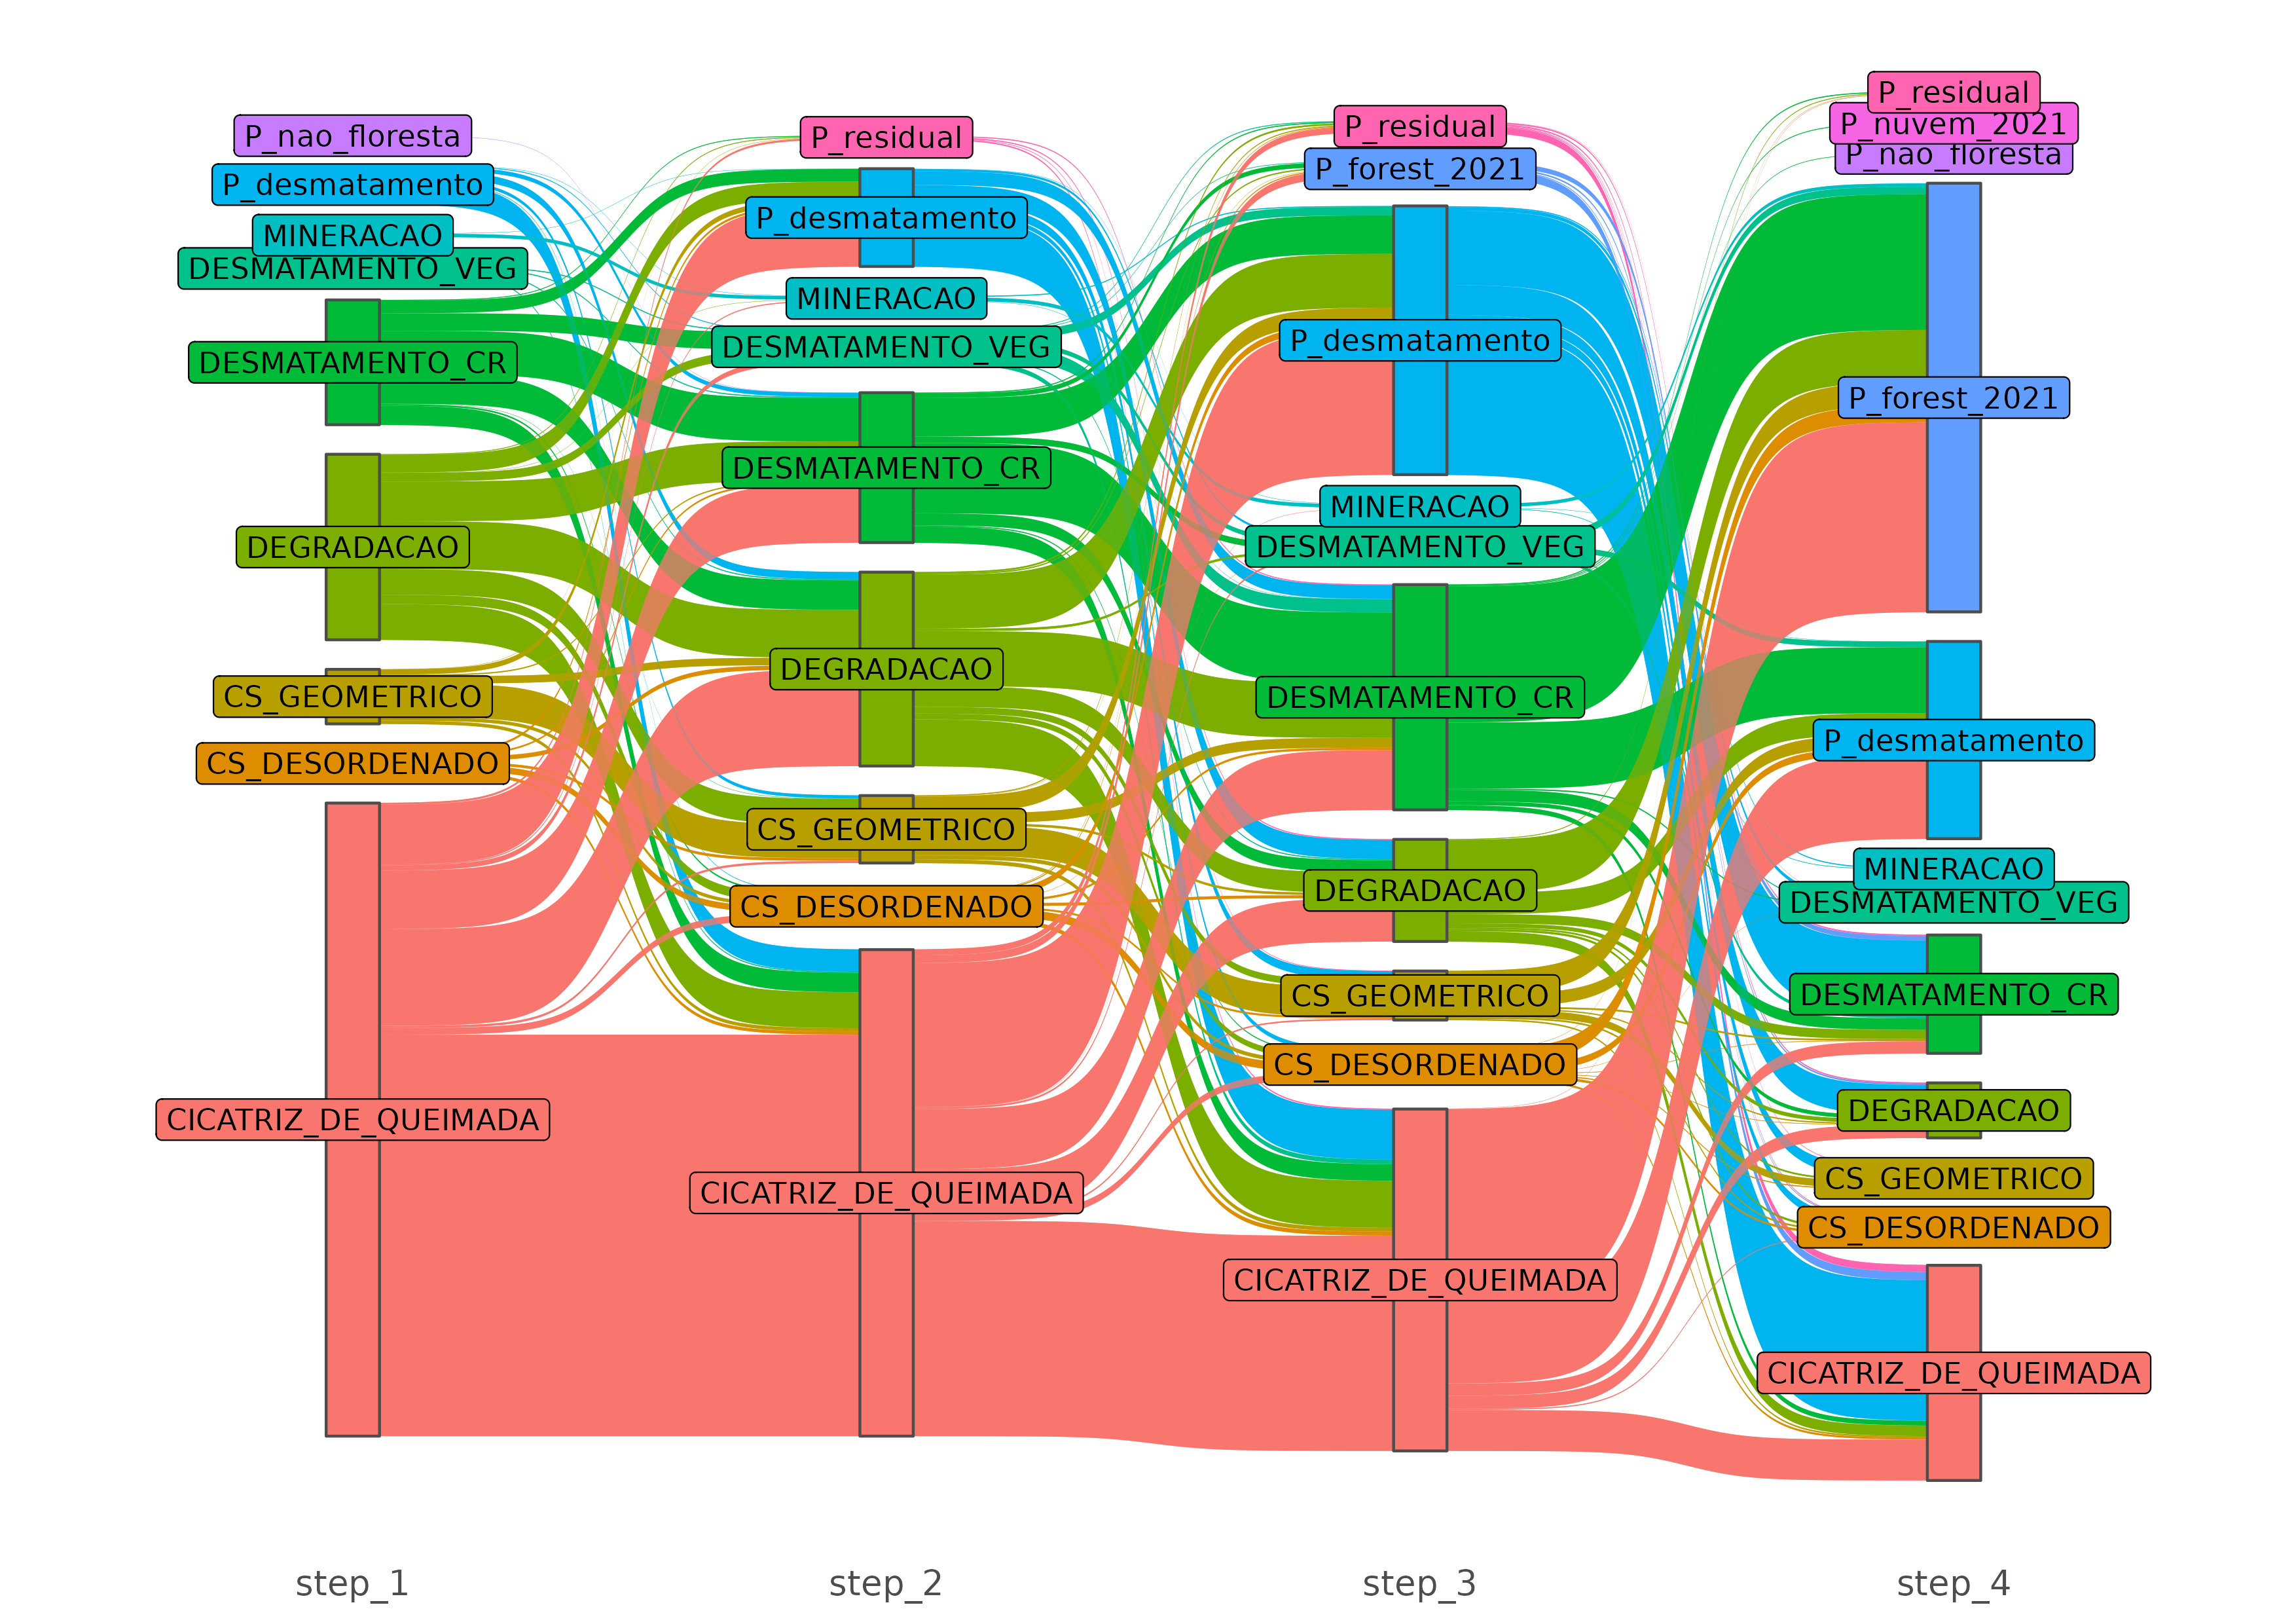
\includegraphics[width=0.65\linewidth]
        {./figures/plot_deter_prodes_subarea_trajectory_4.png}
        \caption{Tajectory of subareas with 4 wanings.}
        \label{fig:deter_prodes_subarea_trajectory_4}
    \end{figure}
\end{frame}

\begin{frame}[allowframebreaks]
    \frametitle{DETER \& PRODES - Top 10 trajectories (4 warnings)}
    \begingroup\fontsize{7}{9}\selectfont

\begin{longtabu} to \linewidth {>{\raggedright}X>{\raggedright}X>{\raggedright}X>{\raggedright}X>{\raggedleft}X>{\raggedleft}X}
\toprule
position\_1 & position\_2 & position\_3 & position\_4 & n\_traj & subarea\_ha\\
\midrule
\cellcolor{gray!6}{Cicatriz de queimada} & \cellcolor{gray!6}{Cicatriz de queimada} & \cellcolor{gray!6}{Cicatriz de queimada} & \cellcolor{gray!6}{P desmatamento} & \cellcolor{gray!6}{236} & \cellcolor{gray!6}{10783.9}\\
\cmidrule{1-6}
Cicatriz de queimada & Cicatriz de queimada & Cicatriz de queimada & P forest 2021 & 524 & 32093.7\\
\cmidrule{1-6}
\cellcolor{gray!6}{Cicatriz de queimada} & \cellcolor{gray!6}{Cicatriz de queimada} & \cellcolor{gray!6}{Cs desordenado} & \cellcolor{gray!6}{P desmatamento} & \cellcolor{gray!6}{5} & \cellcolor{gray!6}{137.3}\\
\cmidrule{1-6}
Cicatriz de queimada & Cicatriz de queimada & Cs desordenado & P forest 2021 & 8 & 277.2\\
\cmidrule{1-6}
\cellcolor{gray!6}{Cicatriz de queimada} & \cellcolor{gray!6}{Cicatriz de queimada} & \cellcolor{gray!6}{Degradacao} & \cellcolor{gray!6}{P desmatamento} & \cellcolor{gray!6}{30} & \cellcolor{gray!6}{1024.3}\\
\cmidrule{1-6}
Cicatriz de queimada & Cicatriz de queimada & Degradacao & P forest 2021 & 102 & 5222.6\\
\cmidrule{1-6}
\cellcolor{gray!6}{Cicatriz de queimada} & \cellcolor{gray!6}{Cicatriz de queimada} & \cellcolor{gray!6}{Desmatamento cr} & \cellcolor{gray!6}{P desmatamento} & \cellcolor{gray!6}{63} & \cellcolor{gray!6}{1689.3}\\
\cmidrule{1-6}
Cicatriz de queimada & Cicatriz de queimada & Desmatamento cr & P forest 2021 & 119 & 2210.2\\
\cmidrule{1-6}
\cellcolor{gray!6}{Cicatriz de queimada} & \cellcolor{gray!6}{Cicatriz de queimada} & \cellcolor{gray!6}{Desmatamento cr} & \cellcolor{gray!6}{P residual} & \cellcolor{gray!6}{2} & \cellcolor{gray!6}{21.1}\\
\cmidrule{1-6}
Cicatriz de queimada & Cicatriz de queimada & Desmatamento veg & P desmatamento & 2 & 29.7\\
\cmidrule{1-6}
\cellcolor{gray!6}{Cicatriz de queimada} & \cellcolor{gray!6}{Cicatriz de queimada} & \cellcolor{gray!6}{Desmatamento veg} & \cellcolor{gray!6}{P forest 2021} & \cellcolor{gray!6}{4} & \cellcolor{gray!6}{70.3}\\
\cmidrule{1-6}
Cicatriz de queimada & Cicatriz de queimada & Mineracao & P forest 2021 & 1 & 3.9\\
\cmidrule{1-6}
\cellcolor{gray!6}{Cicatriz de queimada} & \cellcolor{gray!6}{Cicatriz de queimada} & \cellcolor{gray!6}{P desmatamento} & \cellcolor{gray!6}{Cicatriz de queimada} & \cellcolor{gray!6}{387} & \cellcolor{gray!6}{21441.9}\\
\cmidrule{1-6}
Cicatriz de queimada & Cicatriz de queimada & P desmatamento & Cs desordenado & 6 & 133.0\\
\cmidrule{1-6}
\cellcolor{gray!6}{Cicatriz de queimada} & \cellcolor{gray!6}{Cicatriz de queimada} & \cellcolor{gray!6}{P desmatamento} & \cellcolor{gray!6}{Degradacao} & \cellcolor{gray!6}{60} & \cellcolor{gray!6}{1691.6}\\
\cmidrule{1-6}
Cicatriz de queimada & Cicatriz de queimada & P desmatamento & Desmatamento cr & 79 & 1618.8\\
\cmidrule{1-6}
\cellcolor{gray!6}{Cicatriz de queimada} & \cellcolor{gray!6}{Cicatriz de queimada} & \cellcolor{gray!6}{P desmatamento} & \cellcolor{gray!6}{Desmatamento veg} & \cellcolor{gray!6}{1} & \cellcolor{gray!6}{15.8}\\
\cmidrule{1-6}
Cicatriz de queimada & Cicatriz de queimada & P forest 2021 & Cicatriz de queimada & 21 & 199.1\\
\cmidrule{1-6}
\cellcolor{gray!6}{Cicatriz de queimada} & \cellcolor{gray!6}{Cicatriz de queimada} & \cellcolor{gray!6}{P forest 2021} & \cellcolor{gray!6}{Cs desordenado} & \cellcolor{gray!6}{1} & \cellcolor{gray!6}{17.8}\\
\cmidrule{1-6}
Cicatriz de queimada & Cicatriz de queimada & P forest 2021 & Degradacao & 4 & 98.9\\
\cmidrule{1-6}
\cellcolor{gray!6}{Cicatriz de queimada} & \cellcolor{gray!6}{Cicatriz de queimada} & \cellcolor{gray!6}{P forest 2021} & \cellcolor{gray!6}{Desmatamento cr} & \cellcolor{gray!6}{1} & \cellcolor{gray!6}{3.6}\\
\cmidrule{1-6}
Cicatriz de queimada & Cicatriz de queimada & P residual & Cicatriz de queimada & 20 & 1271.7\\
\cmidrule{1-6}
\cellcolor{gray!6}{Cicatriz de queimada} & \cellcolor{gray!6}{Cicatriz de queimada} & \cellcolor{gray!6}{P residual} & \cellcolor{gray!6}{Cs desordenado} & \cellcolor{gray!6}{1} & \cellcolor{gray!6}{81.7}\\
\cmidrule{1-6}
Cicatriz de queimada & Cicatriz de queimada & P residual & Desmatamento cr & 2 & 7.8\\
\cmidrule{1-6}
\cellcolor{gray!6}{Cicatriz de queimada} & \cellcolor{gray!6}{Cs desordenado} & \cellcolor{gray!6}{Cicatriz de queimada} & \cellcolor{gray!6}{P desmatamento} & \cellcolor{gray!6}{3} & \cellcolor{gray!6}{202.2}\\
\cmidrule{1-6}
Cicatriz de queimada & Cs desordenado & Cicatriz de queimada & P forest 2021 & 7 & 150.9\\
\cmidrule{1-6}
\cellcolor{gray!6}{Cicatriz de queimada} & \cellcolor{gray!6}{Cs desordenado} & \cellcolor{gray!6}{Cs desordenado} & \cellcolor{gray!6}{P forest 2021} & \cellcolor{gray!6}{5} & \cellcolor{gray!6}{86.4}\\
\cmidrule{1-6}
Cicatriz de queimada & Cs desordenado & Desmatamento cr & P forest 2021 & 3 & 30.1\\
\cmidrule{1-6}
\cellcolor{gray!6}{Cicatriz de queimada} & \cellcolor{gray!6}{Cs desordenado} & \cellcolor{gray!6}{P desmatamento} & \cellcolor{gray!6}{Cicatriz de queimada} & \cellcolor{gray!6}{2} & \cellcolor{gray!6}{20.5}\\
\cmidrule{1-6}
Cicatriz de queimada & Cs desordenado & P desmatamento & Cs desordenado & 2 & 17.7\\
\cmidrule{1-6}
\cellcolor{gray!6}{Cicatriz de queimada} & \cellcolor{gray!6}{Cs desordenado} & \cellcolor{gray!6}{P desmatamento} & \cellcolor{gray!6}{Degradacao} & \cellcolor{gray!6}{2} & \cellcolor{gray!6}{15.3}\\
\cmidrule{1-6}
Cicatriz de queimada & Cs desordenado & P desmatamento & Desmatamento cr & 4 & 49.1\\
\cmidrule{1-6}
\cellcolor{gray!6}{Cicatriz de queimada} & \cellcolor{gray!6}{Cs geometrico} & \cellcolor{gray!6}{Cicatriz de queimada} & \cellcolor{gray!6}{P forest 2021} & \cellcolor{gray!6}{1} & \cellcolor{gray!6}{9.0}\\
\cmidrule{1-6}
Cicatriz de queimada & Cs geometrico & Cs geometrico & P desmatamento & 2 & 18.9\\
\cmidrule{1-6}
\cellcolor{gray!6}{Cicatriz de queimada} & \cellcolor{gray!6}{Cs geometrico} & \cellcolor{gray!6}{Cs geometrico} & \cellcolor{gray!6}{P forest 2021} & \cellcolor{gray!6}{3} & \cellcolor{gray!6}{274.5}\\
\cmidrule{1-6}
Cicatriz de queimada & Cs geometrico & Degradacao & P desmatamento & 1 & 4.2\\
\cmidrule{1-6}
\cellcolor{gray!6}{Cicatriz de queimada} & \cellcolor{gray!6}{Cs geometrico} & \cellcolor{gray!6}{Degradacao} & \cellcolor{gray!6}{P forest 2021} & \cellcolor{gray!6}{1} & \cellcolor{gray!6}{5.2}\\
\cmidrule{1-6}
Cicatriz de queimada & Cs geometrico & P desmatamento & Degradacao & 1 & 183.8\\
\cmidrule{1-6}
\cellcolor{gray!6}{Cicatriz de queimada} & \cellcolor{gray!6}{Degradacao} & \cellcolor{gray!6}{Cicatriz de queimada} & \cellcolor{gray!6}{P desmatamento} & \cellcolor{gray!6}{42} & \cellcolor{gray!6}{1161.8}\\
\cmidrule{1-6}
Cicatriz de queimada & Degradacao & Cicatriz de queimada & P forest 2021 & 102 & 4678.7\\
\cmidrule{1-6}
\cellcolor{gray!6}{Cicatriz de queimada} & \cellcolor{gray!6}{Degradacao} & \cellcolor{gray!6}{Cs desordenado} & \cellcolor{gray!6}{P forest 2021} & \cellcolor{gray!6}{2} & \cellcolor{gray!6}{23.3}\\
\cmidrule{1-6}
Cicatriz de queimada & Degradacao & Cs geometrico & P forest 2021 & 1 & 8.2\\
\cmidrule{1-6}
\cellcolor{gray!6}{Cicatriz de queimada} & \cellcolor{gray!6}{Degradacao} & \cellcolor{gray!6}{Degradacao} & \cellcolor{gray!6}{P desmatamento} & \cellcolor{gray!6}{11} & \cellcolor{gray!6}{291.7}\\
\cmidrule{1-6}
Cicatriz de queimada & Degradacao & Degradacao & P forest 2021 & 23 & 542.4\\
\cmidrule{1-6}
\cellcolor{gray!6}{Cicatriz de queimada} & \cellcolor{gray!6}{Degradacao} & \cellcolor{gray!6}{Degradacao} & \cellcolor{gray!6}{P residual} & \cellcolor{gray!6}{1} & \cellcolor{gray!6}{17.0}\\
\cmidrule{1-6}
Cicatriz de queimada & Degradacao & Desmatamento cr & P desmatamento & 28 & 331.0\\
\cmidrule{1-6}
\cellcolor{gray!6}{Cicatriz de queimada} & \cellcolor{gray!6}{Degradacao} & \cellcolor{gray!6}{Desmatamento cr} & \cellcolor{gray!6}{P forest 2021} & \cellcolor{gray!6}{57} & \cellcolor{gray!6}{777.4}\\
\cmidrule{1-6}
Cicatriz de queimada & Degradacao & Desmatamento cr & P nuvem 2021 & 1 & 3.6\\
\cmidrule{1-6}
\cellcolor{gray!6}{Cicatriz de queimada} & \cellcolor{gray!6}{Degradacao} & \cellcolor{gray!6}{Desmatamento veg} & \cellcolor{gray!6}{P desmatamento} & \cellcolor{gray!6}{1} & \cellcolor{gray!6}{6.0}\\
\cmidrule{1-6}
Cicatriz de queimada & Degradacao & Desmatamento veg & P forest 2021 & 1 & 32.3\\
\cmidrule{1-6}
\cellcolor{gray!6}{Cicatriz de queimada} & \cellcolor{gray!6}{Degradacao} & \cellcolor{gray!6}{P desmatamento} & \cellcolor{gray!6}{Cicatriz de queimada} & \cellcolor{gray!6}{75} & \cellcolor{gray!6}{2298.4}\\
\cmidrule{1-6}
Cicatriz de queimada & Degradacao & P desmatamento & Cs desordenado & 3 & 47.3\\
\cmidrule{1-6}
\cellcolor{gray!6}{Cicatriz de queimada} & \cellcolor{gray!6}{Degradacao} & \cellcolor{gray!6}{P desmatamento} & \cellcolor{gray!6}{Cs geometrico} & \cellcolor{gray!6}{2} & \cellcolor{gray!6}{15.6}\\
\cmidrule{1-6}
Cicatriz de queimada & Degradacao & P desmatamento & Degradacao & 22 & 356.6\\
\cmidrule{1-6}
\cellcolor{gray!6}{Cicatriz de queimada} & \cellcolor{gray!6}{Degradacao} & \cellcolor{gray!6}{P desmatamento} & \cellcolor{gray!6}{Desmatamento cr} & \cellcolor{gray!6}{27} & \cellcolor{gray!6}{459.8}\\
\cmidrule{1-6}
Cicatriz de queimada & Degradacao & P forest 2021 & Desmatamento cr & 2 & 17.6\\
\cmidrule{1-6}
\cellcolor{gray!6}{Cicatriz de queimada} & \cellcolor{gray!6}{Degradacao} & \cellcolor{gray!6}{P residual} & \cellcolor{gray!6}{Cicatriz de queimada} & \cellcolor{gray!6}{2} & \cellcolor{gray!6}{65.6}\\
\cmidrule{1-6}
Cicatriz de queimada & Degradacao & P residual & Degradacao & 1 & 13.6\\
\cmidrule{1-6}
\cellcolor{gray!6}{Cicatriz de queimada} & \cellcolor{gray!6}{Desmatamento cr} & \cellcolor{gray!6}{Cicatriz de queimada} & \cellcolor{gray!6}{P desmatamento} & \cellcolor{gray!6}{16} & \cellcolor{gray!6}{222.1}\\
\cmidrule{1-6}
Cicatriz de queimada & Desmatamento cr & Cicatriz de queimada & P forest 2021 & 40 & 719.4\\
\cmidrule{1-6}
\cellcolor{gray!6}{Cicatriz de queimada} & \cellcolor{gray!6}{Desmatamento cr} & \cellcolor{gray!6}{Cicatriz de queimada} & \cellcolor{gray!6}{P residual} & \cellcolor{gray!6}{1} & \cellcolor{gray!6}{3.1}\\
\cmidrule{1-6}
Cicatriz de queimada & Desmatamento cr & Degradacao & P desmatamento & 4 & 30.2\\
\cmidrule{1-6}
\cellcolor{gray!6}{Cicatriz de queimada} & \cellcolor{gray!6}{Desmatamento cr} & \cellcolor{gray!6}{Degradacao} & \cellcolor{gray!6}{P forest 2021} & \cellcolor{gray!6}{11} & \cellcolor{gray!6}{201.7}\\
\cmidrule{1-6}
Cicatriz de queimada & Desmatamento cr & Desmatamento cr & P desmatamento & 24 & 299.4\\
\cmidrule{1-6}
\cellcolor{gray!6}{Cicatriz de queimada} & \cellcolor{gray!6}{Desmatamento cr} & \cellcolor{gray!6}{Desmatamento cr} & \cellcolor{gray!6}{P forest 2021} & \cellcolor{gray!6}{59} & \cellcolor{gray!6}{745.0}\\
\cmidrule{1-6}
Cicatriz de queimada & Desmatamento cr & Desmatamento veg & P desmatamento & 3 & 52.7\\
\cmidrule{1-6}
\cellcolor{gray!6}{Cicatriz de queimada} & \cellcolor{gray!6}{Desmatamento cr} & \cellcolor{gray!6}{Desmatamento veg} & \cellcolor{gray!6}{P forest 2021} & \cellcolor{gray!6}{3} & \cellcolor{gray!6}{92.1}\\
\cmidrule{1-6}
Cicatriz de queimada & Desmatamento cr & P desmatamento & Cicatriz de queimada & 26 & 259.0\\
\cmidrule{1-6}
\cellcolor{gray!6}{Cicatriz de queimada} & \cellcolor{gray!6}{Desmatamento cr} & \cellcolor{gray!6}{P desmatamento} & \cellcolor{gray!6}{Degradacao} & \cellcolor{gray!6}{7} & \cellcolor{gray!6}{50.7}\\
\cmidrule{1-6}
Cicatriz de queimada & Desmatamento cr & P desmatamento & Desmatamento cr & 36 & 482.5\\
\cmidrule{1-6}
\cellcolor{gray!6}{Cicatriz de queimada} & \cellcolor{gray!6}{Desmatamento cr} & \cellcolor{gray!6}{P desmatamento} & \cellcolor{gray!6}{Desmatamento veg} & \cellcolor{gray!6}{1} & \cellcolor{gray!6}{7.0}\\
\cmidrule{1-6}
Cicatriz de queimada & Desmatamento cr & P forest 2021 & Cicatriz de queimada & 9 & 140.1\\
\cmidrule{1-6}
\cellcolor{gray!6}{Cicatriz de queimada} & \cellcolor{gray!6}{Desmatamento cr} & \cellcolor{gray!6}{P forest 2021} & \cellcolor{gray!6}{Desmatamento cr} & \cellcolor{gray!6}{3} & \cellcolor{gray!6}{21.7}\\
\cmidrule{1-6}
Cicatriz de queimada & Desmatamento cr & P residual & Cicatriz de queimada & 2 & 21.0\\
\cmidrule{1-6}
\cellcolor{gray!6}{Cicatriz de queimada} & \cellcolor{gray!6}{Desmatamento veg} & \cellcolor{gray!6}{Cicatriz de queimada} & \cellcolor{gray!6}{P desmatamento} & \cellcolor{gray!6}{1} & \cellcolor{gray!6}{8.2}\\
\cmidrule{1-6}
Cicatriz de queimada & Desmatamento veg & Cicatriz de queimada & P forest 2021 & 4 & 46.5\\
\cmidrule{1-6}
\cellcolor{gray!6}{Cicatriz de queimada} & \cellcolor{gray!6}{Desmatamento veg} & \cellcolor{gray!6}{Degradacao} & \cellcolor{gray!6}{P desmatamento} & \cellcolor{gray!6}{1} & \cellcolor{gray!6}{3.7}\\
\cmidrule{1-6}
Cicatriz de queimada & Desmatamento veg & Desmatamento cr & P desmatamento & 1 & 17.4\\
\cmidrule{1-6}
\cellcolor{gray!6}{Cicatriz de queimada} & \cellcolor{gray!6}{Desmatamento veg} & \cellcolor{gray!6}{Desmatamento cr} & \cellcolor{gray!6}{P forest 2021} & \cellcolor{gray!6}{5} & \cellcolor{gray!6}{67.4}\\
\cmidrule{1-6}
Cicatriz de queimada & Desmatamento veg & Desmatamento veg & P forest 2021 & 1 & 3.5\\
\cmidrule{1-6}
\cellcolor{gray!6}{Cicatriz de queimada} & \cellcolor{gray!6}{Desmatamento veg} & \cellcolor{gray!6}{P desmatamento} & \cellcolor{gray!6}{Cicatriz de queimada} & \cellcolor{gray!6}{2} & \cellcolor{gray!6}{9.7}\\
\cmidrule{1-6}
Cicatriz de queimada & Desmatamento veg & P desmatamento & Degradacao & 1 & 6.1\\
\cmidrule{1-6}
\cellcolor{gray!6}{Cicatriz de queimada} & \cellcolor{gray!6}{Desmatamento veg} & \cellcolor{gray!6}{P desmatamento} & \cellcolor{gray!6}{Desmatamento cr} & \cellcolor{gray!6}{4} & \cellcolor{gray!6}{65.4}\\
\cmidrule{1-6}
Cicatriz de queimada & Desmatamento veg & P forest 2021 & Desmatamento cr & 1 & 6.7\\
\cmidrule{1-6}
\cellcolor{gray!6}{Cicatriz de queimada} & \cellcolor{gray!6}{Mineracao} & \cellcolor{gray!6}{Mineracao} & \cellcolor{gray!6}{P forest 2021} & \cellcolor{gray!6}{4} & \cellcolor{gray!6}{19.4}\\
\cmidrule{1-6}
Cicatriz de queimada & P desmatamento & Cicatriz de queimada & Cicatriz de queimada & 116 & 5683.2\\
\cmidrule{1-6}
\cellcolor{gray!6}{Cicatriz de queimada} & \cellcolor{gray!6}{P desmatamento} & \cellcolor{gray!6}{Cicatriz de queimada} & \cellcolor{gray!6}{Degradacao} & \cellcolor{gray!6}{33} & \cellcolor{gray!6}{508.2}\\
\cmidrule{1-6}
Cicatriz de queimada & P desmatamento & Cicatriz de queimada & Desmatamento cr & 27 & 367.2\\
\cmidrule{1-6}
\cellcolor{gray!6}{Cicatriz de queimada} & \cellcolor{gray!6}{P desmatamento} & \cellcolor{gray!6}{Cs desordenado} & \cellcolor{gray!6}{Cicatriz de queimada} & \cellcolor{gray!6}{1} & \cellcolor{gray!6}{15.0}\\
\cmidrule{1-6}
Cicatriz de queimada & P desmatamento & Cs desordenado & Cs desordenado & 1 & 13.6\\
\cmidrule{1-6}
\cellcolor{gray!6}{Cicatriz de queimada} & \cellcolor{gray!6}{P desmatamento} & \cellcolor{gray!6}{Cs desordenado} & \cellcolor{gray!6}{Degradacao} & \cellcolor{gray!6}{1} & \cellcolor{gray!6}{5.9}\\
\cmidrule{1-6}
Cicatriz de queimada & P desmatamento & Cs desordenado & Desmatamento cr & 1 & 4.1\\
\cmidrule{1-6}
\cellcolor{gray!6}{Cicatriz de queimada} & \cellcolor{gray!6}{P desmatamento} & \cellcolor{gray!6}{Cs geometrico} & \cellcolor{gray!6}{Cicatriz de queimada} & \cellcolor{gray!6}{1} & \cellcolor{gray!6}{3.7}\\
\cmidrule{1-6}
Cicatriz de queimada & P desmatamento & Cs geometrico & Cs geometrico & 1 & 14.2\\
\cmidrule{1-6}
\cellcolor{gray!6}{Cicatriz de queimada} & \cellcolor{gray!6}{P desmatamento} & \cellcolor{gray!6}{Cs geometrico} & \cellcolor{gray!6}{Degradacao} & \cellcolor{gray!6}{1} & \cellcolor{gray!6}{17.2}\\
\cmidrule{1-6}
Cicatriz de queimada & P desmatamento & Degradacao & Cicatriz de queimada & 26 & 326.0\\
\cmidrule{1-6}
\cellcolor{gray!6}{Cicatriz de queimada} & \cellcolor{gray!6}{P desmatamento} & \cellcolor{gray!6}{Degradacao} & \cellcolor{gray!6}{Cs geometrico} & \cellcolor{gray!6}{1} & \cellcolor{gray!6}{21.5}\\
\cmidrule{1-6}
Cicatriz de queimada & P desmatamento & Degradacao & Degradacao & 4 & 133.2\\
\cmidrule{1-6}
\cellcolor{gray!6}{Cicatriz de queimada} & \cellcolor{gray!6}{P desmatamento} & \cellcolor{gray!6}{Degradacao} & \cellcolor{gray!6}{Desmatamento cr} & \cellcolor{gray!6}{9} & \cellcolor{gray!6}{94.1}\\
\cmidrule{1-6}
Cicatriz de queimada & P desmatamento & Desmatamento cr & Cicatriz de queimada & 11 & 136.3\\
\cmidrule{1-6}
\cellcolor{gray!6}{Cicatriz de queimada} & \cellcolor{gray!6}{P desmatamento} & \cellcolor{gray!6}{Desmatamento cr} & \cellcolor{gray!6}{Degradacao} & \cellcolor{gray!6}{4} & \cellcolor{gray!6}{33.2}\\
\cmidrule{1-6}
Cicatriz de queimada & P desmatamento & Desmatamento cr & Desmatamento cr & 10 & 65.7\\
\cmidrule{1-6}
\cellcolor{gray!6}{Cicatriz de queimada} & \cellcolor{gray!6}{P desmatamento} & \cellcolor{gray!6}{Desmatamento cr} & \cellcolor{gray!6}{Desmatamento veg} & \cellcolor{gray!6}{2} & \cellcolor{gray!6}{9.8}\\
\cmidrule{1-6}
Cicatriz de queimada & P residual & Cicatriz de queimada & Cicatriz de queimada & 1 & 3.9\\
\cmidrule{1-6}
\cellcolor{gray!6}{Cicatriz de queimada} & \cellcolor{gray!6}{P residual} & \cellcolor{gray!6}{Cicatriz de queimada} & \cellcolor{gray!6}{Degradacao} & \cellcolor{gray!6}{3} & \cellcolor{gray!6}{15.3}\\
\cmidrule{1-6}
Cicatriz de queimada & P residual & Cicatriz de queimada & Desmatamento cr & 1 & 17.4\\
\cmidrule{1-6}
\cellcolor{gray!6}{Cicatriz de queimada} & \cellcolor{gray!6}{P residual} & \cellcolor{gray!6}{Degradacao} & \cellcolor{gray!6}{Degradacao} & \cellcolor{gray!6}{1} & \cellcolor{gray!6}{10.6}\\
\cmidrule{1-6}
Cicatriz de queimada & P residual & Desmatamento cr & Cicatriz de queimada & 2 & 10.4\\
\cmidrule{1-6}
\cellcolor{gray!6}{Cs desordenado} & \cellcolor{gray!6}{Cicatriz de queimada} & \cellcolor{gray!6}{Cicatriz de queimada} & \cellcolor{gray!6}{P desmatamento} & \cellcolor{gray!6}{2} & \cellcolor{gray!6}{102.1}\\
\cmidrule{1-6}
Cs desordenado & Cicatriz de queimada & Cicatriz de queimada & P forest 2021 & 3 & 315.2\\
\cmidrule{1-6}
\cellcolor{gray!6}{Cs desordenado} & \cellcolor{gray!6}{Cicatriz de queimada} & \cellcolor{gray!6}{Cs desordenado} & \cellcolor{gray!6}{P desmatamento} & \cellcolor{gray!6}{2} & \cellcolor{gray!6}{27.6}\\
\cmidrule{1-6}
Cs desordenado & Cicatriz de queimada & Desmatamento cr & P desmatamento & 2 & 23.5\\
\cmidrule{1-6}
\cellcolor{gray!6}{Cs desordenado} & \cellcolor{gray!6}{Cicatriz de queimada} & \cellcolor{gray!6}{Desmatamento cr} & \cellcolor{gray!6}{P forest 2021} & \cellcolor{gray!6}{1} & \cellcolor{gray!6}{39.2}\\
\cmidrule{1-6}
Cs desordenado & Cicatriz de queimada & P desmatamento & Cicatriz de queimada & 3 & 47.4\\
\cmidrule{1-6}
\cellcolor{gray!6}{Cs desordenado} & \cellcolor{gray!6}{Cs desordenado} & \cellcolor{gray!6}{Cs desordenado} & \cellcolor{gray!6}{P desmatamento} & \cellcolor{gray!6}{6} & \cellcolor{gray!6}{195.9}\\
\cmidrule{1-6}
Cs desordenado & Cs desordenado & Cs desordenado & P forest 2021 & 7 & 238.5\\
\cmidrule{1-6}
\cellcolor{gray!6}{Cs desordenado} & \cellcolor{gray!6}{Cs desordenado} & \cellcolor{gray!6}{Cs geometrico} & \cellcolor{gray!6}{P forest 2021} & \cellcolor{gray!6}{1} & \cellcolor{gray!6}{4.3}\\
\cmidrule{1-6}
Cs desordenado & Cs desordenado & Degradacao & P desmatamento & 1 & 10.2\\
\cmidrule{1-6}
\cellcolor{gray!6}{Cs desordenado} & \cellcolor{gray!6}{Cs desordenado} & \cellcolor{gray!6}{Degradacao} & \cellcolor{gray!6}{P forest 2021} & \cellcolor{gray!6}{1} & \cellcolor{gray!6}{7.8}\\
\cmidrule{1-6}
Cs desordenado & Cs desordenado & Desmatamento cr & P forest 2021 & 1 & 4.9\\
\cmidrule{1-6}
\cellcolor{gray!6}{Cs desordenado} & \cellcolor{gray!6}{Cs desordenado} & \cellcolor{gray!6}{P desmatamento} & \cellcolor{gray!6}{Cicatriz de queimada} & \cellcolor{gray!6}{2} & \cellcolor{gray!6}{18.0}\\
\cmidrule{1-6}
Cs desordenado & Cs desordenado & P desmatamento & Cs desordenado & 4 & 127.7\\
\cmidrule{1-6}
\cellcolor{gray!6}{Cs desordenado} & \cellcolor{gray!6}{Cs desordenado} & \cellcolor{gray!6}{P desmatamento} & \cellcolor{gray!6}{Degradacao} & \cellcolor{gray!6}{1} & \cellcolor{gray!6}{25.1}\\
\cmidrule{1-6}
Cs desordenado & Cs desordenado & P forest 2021 & Cs desordenado & 2 & 109.5\\
\cmidrule{1-6}
\cellcolor{gray!6}{Cs desordenado} & \cellcolor{gray!6}{Cs geometrico} & \cellcolor{gray!6}{Cicatriz de queimada} & \cellcolor{gray!6}{P forest 2021} & \cellcolor{gray!6}{1} & \cellcolor{gray!6}{14.0}\\
\cmidrule{1-6}
Cs desordenado & Cs geometrico & Cs desordenado & P forest 2021 & 3 & 115.5\\
\cmidrule{1-6}
\cellcolor{gray!6}{Cs desordenado} & \cellcolor{gray!6}{Cs geometrico} & \cellcolor{gray!6}{Cs geometrico} & \cellcolor{gray!6}{P desmatamento} & \cellcolor{gray!6}{1} & \cellcolor{gray!6}{135.1}\\
\cmidrule{1-6}
Cs desordenado & Cs geometrico & Cs geometrico & P forest 2021 & 1 & 41.2\\
\cmidrule{1-6}
\cellcolor{gray!6}{Cs desordenado} & \cellcolor{gray!6}{Cs geometrico} & \cellcolor{gray!6}{Degradacao} & \cellcolor{gray!6}{P desmatamento} & \cellcolor{gray!6}{1} & \cellcolor{gray!6}{11.6}\\
\cmidrule{1-6}
Cs desordenado & Cs geometrico & P desmatamento & Cicatriz de queimada & 3 & 130.9\\
\cmidrule{1-6}
\cellcolor{gray!6}{Cs desordenado} & \cellcolor{gray!6}{Cs geometrico} & \cellcolor{gray!6}{P desmatamento} & \cellcolor{gray!6}{Cs desordenado} & \cellcolor{gray!6}{1} & \cellcolor{gray!6}{68.6}\\
\cmidrule{1-6}
Cs desordenado & Degradacao & Cicatriz de queimada & P desmatamento & 1 & 5.7\\
\cmidrule{1-6}
\cellcolor{gray!6}{Cs desordenado} & \cellcolor{gray!6}{Degradacao} & \cellcolor{gray!6}{Cicatriz de queimada} & \cellcolor{gray!6}{P forest 2021} & \cellcolor{gray!6}{4} & \cellcolor{gray!6}{21.6}\\
\cmidrule{1-6}
Cs desordenado & Degradacao & Cs desordenado & P forest 2021 & 3 & 553.6\\
\cmidrule{1-6}
\cellcolor{gray!6}{Cs desordenado} & \cellcolor{gray!6}{Degradacao} & \cellcolor{gray!6}{Cs geometrico} & \cellcolor{gray!6}{P forest 2021} & \cellcolor{gray!6}{1} & \cellcolor{gray!6}{3.9}\\
\cmidrule{1-6}
Cs desordenado & Degradacao & Degradacao & P forest 2021 & 1 & 3.4\\
\cmidrule{1-6}
\cellcolor{gray!6}{Cs desordenado} & \cellcolor{gray!6}{Degradacao} & \cellcolor{gray!6}{Desmatamento cr} & \cellcolor{gray!6}{P desmatamento} & \cellcolor{gray!6}{1} & \cellcolor{gray!6}{5.7}\\
\cmidrule{1-6}
Cs desordenado & Degradacao & Desmatamento cr & P forest 2021 & 1 & 12.1\\
\cmidrule{1-6}
\cellcolor{gray!6}{Cs desordenado} & \cellcolor{gray!6}{Degradacao} & \cellcolor{gray!6}{P desmatamento} & \cellcolor{gray!6}{Cs desordenado} & \cellcolor{gray!6}{1} & \cellcolor{gray!6}{16.2}\\
\cmidrule{1-6}
Cs desordenado & Degradacao & P desmatamento & Cs geometrico & 1 & 7.1\\
\cmidrule{1-6}
\cellcolor{gray!6}{Cs desordenado} & \cellcolor{gray!6}{Degradacao} & \cellcolor{gray!6}{P desmatamento} & \cellcolor{gray!6}{Degradacao} & \cellcolor{gray!6}{1} & \cellcolor{gray!6}{15.9}\\
\cmidrule{1-6}
Cs desordenado & Degradacao & P desmatamento & Desmatamento cr & 2 & 17.6\\
\cmidrule{1-6}
\cellcolor{gray!6}{Cs desordenado} & \cellcolor{gray!6}{Degradacao} & \cellcolor{gray!6}{P residual} & \cellcolor{gray!6}{Cs desordenado} & \cellcolor{gray!6}{1} & \cellcolor{gray!6}{30.1}\\
\cmidrule{1-6}
Cs desordenado & Desmatamento cr & Cicatriz de queimada & P desmatamento & 1 & 3.4\\
\cmidrule{1-6}
\cellcolor{gray!6}{Cs desordenado} & \cellcolor{gray!6}{Desmatamento cr} & \cellcolor{gray!6}{Desmatamento cr} & \cellcolor{gray!6}{P forest 2021} & \cellcolor{gray!6}{4} & \cellcolor{gray!6}{88.1}\\
\cmidrule{1-6}
Cs desordenado & Desmatamento cr & Desmatamento veg & P desmatamento & 1 & 3.7\\
\cmidrule{1-6}
\cellcolor{gray!6}{Cs desordenado} & \cellcolor{gray!6}{Desmatamento cr} & \cellcolor{gray!6}{P desmatamento} & \cellcolor{gray!6}{Desmatamento cr} & \cellcolor{gray!6}{1} & \cellcolor{gray!6}{18.6}\\
\cmidrule{1-6}
Cs desordenado & P desmatamento & Cs desordenado & Cs desordenado & 2 & 20.7\\
\cmidrule{1-6}
\cellcolor{gray!6}{Cs desordenado} & \cellcolor{gray!6}{P desmatamento} & \cellcolor{gray!6}{Cs geometrico} & \cellcolor{gray!6}{Cs geometrico} & \cellcolor{gray!6}{1} & \cellcolor{gray!6}{344.6}\\
\cmidrule{1-6}
Cs desordenado & P desmatamento & Degradacao & Cs desordenado & 3 & 140.0\\
\cmidrule{1-6}
\cellcolor{gray!6}{Cs desordenado} & \cellcolor{gray!6}{P desmatamento} & \cellcolor{gray!6}{Degradacao} & \cellcolor{gray!6}{Desmatamento cr} & \cellcolor{gray!6}{1} & \cellcolor{gray!6}{4.4}\\
\cmidrule{1-6}
Cs desordenado & P desmatamento & Desmatamento cr & Desmatamento cr & 1 & 3.2\\
\cmidrule{1-6}
\cellcolor{gray!6}{Cs desordenado} & \cellcolor{gray!6}{P desmatamento} & \cellcolor{gray!6}{Desmatamento veg} & \cellcolor{gray!6}{Desmatamento cr} & \cellcolor{gray!6}{1} & \cellcolor{gray!6}{5.1}\\
\cmidrule{1-6}
Cs geometrico & Cicatriz de queimada & Cicatriz de queimada & P desmatamento & 4 & 214.8\\
\cmidrule{1-6}
\cellcolor{gray!6}{Cs geometrico} & \cellcolor{gray!6}{Cicatriz de queimada} & \cellcolor{gray!6}{Cicatriz de queimada} & \cellcolor{gray!6}{P forest 2021} & \cellcolor{gray!6}{1} & \cellcolor{gray!6}{5.3}\\
\cmidrule{1-6}
Cs geometrico & Cicatriz de queimada & Cs geometrico & P forest 2021 & 1 & 3.3\\
\cmidrule{1-6}
\cellcolor{gray!6}{Cs geometrico} & \cellcolor{gray!6}{Cicatriz de queimada} & \cellcolor{gray!6}{Degradacao} & \cellcolor{gray!6}{P desmatamento} & \cellcolor{gray!6}{2} & \cellcolor{gray!6}{7.9}\\
\cmidrule{1-6}
Cs geometrico & Cicatriz de queimada & Degradacao & P forest 2021 & 5 & 41.2\\
\cmidrule{1-6}
\cellcolor{gray!6}{Cs geometrico} & \cellcolor{gray!6}{Cicatriz de queimada} & \cellcolor{gray!6}{P desmatamento} & \cellcolor{gray!6}{Cicatriz de queimada} & \cellcolor{gray!6}{1} & \cellcolor{gray!6}{7.7}\\
\cmidrule{1-6}
Cs geometrico & Cs desordenado & Cicatriz de queimada & P desmatamento & 1 & 38.9\\
\cmidrule{1-6}
\cellcolor{gray!6}{Cs geometrico} & \cellcolor{gray!6}{Cs desordenado} & \cellcolor{gray!6}{Cicatriz de queimada} & \cellcolor{gray!6}{P forest 2021} & \cellcolor{gray!6}{1} & \cellcolor{gray!6}{46.1}\\
\cmidrule{1-6}
Cs geometrico & Cs desordenado & Cs desordenado & P forest 2021 & 3 & 135.1\\
\cmidrule{1-6}
\cellcolor{gray!6}{Cs geometrico} & \cellcolor{gray!6}{Cs desordenado} & \cellcolor{gray!6}{Cs geometrico} & \cellcolor{gray!6}{P desmatamento} & \cellcolor{gray!6}{1} & \cellcolor{gray!6}{3.0}\\
\cmidrule{1-6}
Cs geometrico & Cs desordenado & Cs geometrico & P forest 2021 & 1 & 274.9\\
\cmidrule{1-6}
\cellcolor{gray!6}{Cs geometrico} & \cellcolor{gray!6}{Cs desordenado} & \cellcolor{gray!6}{Degradacao} & \cellcolor{gray!6}{P desmatamento} & \cellcolor{gray!6}{2} & \cellcolor{gray!6}{174.4}\\
\cmidrule{1-6}
Cs geometrico & Cs desordenado & Degradacao & P forest 2021 & 2 & 30.4\\
\cmidrule{1-6}
\cellcolor{gray!6}{Cs geometrico} & \cellcolor{gray!6}{Cs desordenado} & \cellcolor{gray!6}{P desmatamento} & \cellcolor{gray!6}{Cs geometrico} & \cellcolor{gray!6}{1} & \cellcolor{gray!6}{5.7}\\
\cmidrule{1-6}
Cs geometrico & Cs desordenado & P desmatamento & Degradacao & 2 & 121.4\\
\cmidrule{1-6}
\cellcolor{gray!6}{Cs geometrico} & \cellcolor{gray!6}{Cs geometrico} & \cellcolor{gray!6}{Cicatriz de queimada} & \cellcolor{gray!6}{P desmatamento} & \cellcolor{gray!6}{2} & \cellcolor{gray!6}{15.7}\\
\cmidrule{1-6}
Cs geometrico & Cs geometrico & Cicatriz de queimada & P forest 2021 & 3 & 333.4\\
\cmidrule{1-6}
\cellcolor{gray!6}{Cs geometrico} & \cellcolor{gray!6}{Cs geometrico} & \cellcolor{gray!6}{Cs desordenado} & \cellcolor{gray!6}{P forest 2021} & \cellcolor{gray!6}{9} & \cellcolor{gray!6}{200.3}\\
\cmidrule{1-6}
Cs geometrico & Cs geometrico & Cs geometrico & P desmatamento & 23 & 1396.0\\
\cmidrule{1-6}
\cellcolor{gray!6}{Cs geometrico} & \cellcolor{gray!6}{Cs geometrico} & \cellcolor{gray!6}{Cs geometrico} & \cellcolor{gray!6}{P forest 2021} & \cellcolor{gray!6}{47} & \cellcolor{gray!6}{3097.3}\\
\cmidrule{1-6}
Cs geometrico & Cs geometrico & Degradacao & P desmatamento & 1 & 5.3\\
\cmidrule{1-6}
\cellcolor{gray!6}{Cs geometrico} & \cellcolor{gray!6}{Cs geometrico} & \cellcolor{gray!6}{Degradacao} & \cellcolor{gray!6}{P forest 2021} & \cellcolor{gray!6}{2} & \cellcolor{gray!6}{37.0}\\
\cmidrule{1-6}
Cs geometrico & Cs geometrico & Desmatamento cr & P desmatamento & 6 & 234.9\\
\cmidrule{1-6}
\cellcolor{gray!6}{Cs geometrico} & \cellcolor{gray!6}{Cs geometrico} & \cellcolor{gray!6}{Desmatamento cr} & \cellcolor{gray!6}{P forest 2021} & \cellcolor{gray!6}{11} & \cellcolor{gray!6}{321.0}\\
\cmidrule{1-6}
Cs geometrico & Cs geometrico & P desmatamento & Cicatriz de queimada & 6 & 294.5\\
\cmidrule{1-6}
\cellcolor{gray!6}{Cs geometrico} & \cellcolor{gray!6}{Cs geometrico} & \cellcolor{gray!6}{P desmatamento} & \cellcolor{gray!6}{Cs desordenado} & \cellcolor{gray!6}{3} & \cellcolor{gray!6}{94.0}\\
\cmidrule{1-6}
Cs geometrico & Cs geometrico & P desmatamento & Cs geometrico & 18 & 1812.0\\
\cmidrule{1-6}
\cellcolor{gray!6}{Cs geometrico} & \cellcolor{gray!6}{Cs geometrico} & \cellcolor{gray!6}{P desmatamento} & \cellcolor{gray!6}{Degradacao} & \cellcolor{gray!6}{1} & \cellcolor{gray!6}{18.9}\\
\cmidrule{1-6}
Cs geometrico & Cs geometrico & P desmatamento & Desmatamento cr & 7 & 131.0\\
\cmidrule{1-6}
\cellcolor{gray!6}{Cs geometrico} & \cellcolor{gray!6}{Cs geometrico} & \cellcolor{gray!6}{P forest 2021} & \cellcolor{gray!6}{Desmatamento cr} & \cellcolor{gray!6}{1} & \cellcolor{gray!6}{8.3}\\
\cmidrule{1-6}
Cs geometrico & Cs geometrico & P residual & Degradacao & 1 & 13.6\\
\cmidrule{1-6}
\cellcolor{gray!6}{Cs geometrico} & \cellcolor{gray!6}{Degradacao} & \cellcolor{gray!6}{Cicatriz de queimada} & \cellcolor{gray!6}{P forest 2021} & \cellcolor{gray!6}{2} & \cellcolor{gray!6}{17.5}\\
\cmidrule{1-6}
Cs geometrico & Degradacao & Cs desordenado & P forest 2021 & 1 & 118.4\\
\cmidrule{1-6}
\cellcolor{gray!6}{Cs geometrico} & \cellcolor{gray!6}{Degradacao} & \cellcolor{gray!6}{Cs geometrico} & \cellcolor{gray!6}{P desmatamento} & \cellcolor{gray!6}{7} & \cellcolor{gray!6}{522.9}\\
\cmidrule{1-6}
Cs geometrico & Degradacao & Cs geometrico & P forest 2021 & 6 & 160.8\\
\cmidrule{1-6}
\cellcolor{gray!6}{Cs geometrico} & \cellcolor{gray!6}{Degradacao} & \cellcolor{gray!6}{Degradacao} & \cellcolor{gray!6}{P forest 2021} & \cellcolor{gray!6}{2} & \cellcolor{gray!6}{34.6}\\
\cmidrule{1-6}
Cs geometrico & Degradacao & Desmatamento cr & P desmatamento & 2 & 22.9\\
\cmidrule{1-6}
\cellcolor{gray!6}{Cs geometrico} & \cellcolor{gray!6}{Degradacao} & \cellcolor{gray!6}{Desmatamento cr} & \cellcolor{gray!6}{P forest 2021} & \cellcolor{gray!6}{3} & \cellcolor{gray!6}{86.2}\\
\cmidrule{1-6}
Cs geometrico & Degradacao & P desmatamento & Cs geometrico & 5 & 98.5\\
\cmidrule{1-6}
\cellcolor{gray!6}{Cs geometrico} & \cellcolor{gray!6}{Degradacao} & \cellcolor{gray!6}{P desmatamento} & \cellcolor{gray!6}{Desmatamento cr} & \cellcolor{gray!6}{2} & \cellcolor{gray!6}{24.0}\\
\cmidrule{1-6}
Cs geometrico & Degradacao & P residual & Cs geometrico & 1 & 10.5\\
\cmidrule{1-6}
\cellcolor{gray!6}{Cs geometrico} & \cellcolor{gray!6}{Desmatamento cr} & \cellcolor{gray!6}{Cs desordenado} & \cellcolor{gray!6}{P forest 2021} & \cellcolor{gray!6}{2} & \cellcolor{gray!6}{9.3}\\
\cmidrule{1-6}
Cs geometrico & Desmatamento cr & Desmatamento cr & P desmatamento & 1 & 5.2\\
\cmidrule{1-6}
\cellcolor{gray!6}{Cs geometrico} & \cellcolor{gray!6}{Desmatamento cr} & \cellcolor{gray!6}{P desmatamento} & \cellcolor{gray!6}{Desmatamento cr} & \cellcolor{gray!6}{1} & \cellcolor{gray!6}{5.2}\\
\cmidrule{1-6}
Cs geometrico & Desmatamento cr & P desmatamento & Desmatamento veg & 1 & 4.2\\
\cmidrule{1-6}
\cellcolor{gray!6}{Cs geometrico} & \cellcolor{gray!6}{P desmatamento} & \cellcolor{gray!6}{Cs desordenado} & \cellcolor{gray!6}{Cs geometrico} & \cellcolor{gray!6}{1} & \cellcolor{gray!6}{21.5}\\
\cmidrule{1-6}
Cs geometrico & P desmatamento & Cs geometrico & Cicatriz de queimada & 1 & 45.6\\
\cmidrule{1-6}
\cellcolor{gray!6}{Cs geometrico} & \cellcolor{gray!6}{P desmatamento} & \cellcolor{gray!6}{Cs geometrico} & \cellcolor{gray!6}{Cs desordenado} & \cellcolor{gray!6}{3} & \cellcolor{gray!6}{250.4}\\
\cmidrule{1-6}
Cs geometrico & P desmatamento & Cs geometrico & Cs geometrico & 9 & 443.0\\
\cmidrule{1-6}
\cellcolor{gray!6}{Cs geometrico} & \cellcolor{gray!6}{P desmatamento} & \cellcolor{gray!6}{Cs geometrico} & \cellcolor{gray!6}{Desmatamento cr} & \cellcolor{gray!6}{2} & \cellcolor{gray!6}{23.7}\\
\cmidrule{1-6}
Cs geometrico & P desmatamento & Degradacao & Cs desordenado & 1 & 14.3\\
\cmidrule{1-6}
\cellcolor{gray!6}{Cs geometrico} & \cellcolor{gray!6}{P desmatamento} & \cellcolor{gray!6}{Degradacao} & \cellcolor{gray!6}{Cs geometrico} & \cellcolor{gray!6}{3} & \cellcolor{gray!6}{26.4}\\
\cmidrule{1-6}
Cs geometrico & P desmatamento & Degradacao & Desmatamento cr & 2 & 73.7\\
\cmidrule{1-6}
\cellcolor{gray!6}{Cs geometrico} & \cellcolor{gray!6}{P residual} & \cellcolor{gray!6}{Cs geometrico} & \cellcolor{gray!6}{Cs geometrico} & \cellcolor{gray!6}{1} & \cellcolor{gray!6}{222.3}\\
\cmidrule{1-6}
Degradacao & Cicatriz de queimada & Cicatriz de queimada & P desmatamento & 13 & 241.3\\
\cmidrule{1-6}
\cellcolor{gray!6}{Degradacao} & \cellcolor{gray!6}{Cicatriz de queimada} & \cellcolor{gray!6}{Cicatriz de queimada} & \cellcolor{gray!6}{P forest 2021} & \cellcolor{gray!6}{26} & \cellcolor{gray!6}{615.9}\\
\cmidrule{1-6}
Degradacao & Cicatriz de queimada & Cs desordenado & P desmatamento & 4 & 165.0\\
\cmidrule{1-6}
\cellcolor{gray!6}{Degradacao} & \cellcolor{gray!6}{Cicatriz de queimada} & \cellcolor{gray!6}{Cs desordenado} & \cellcolor{gray!6}{P forest 2021} & \cellcolor{gray!6}{6} & \cellcolor{gray!6}{114.2}\\
\cmidrule{1-6}
Degradacao & Cicatriz de queimada & Cs geometrico & P desmatamento & 3 & 19.1\\
\cmidrule{1-6}
\cellcolor{gray!6}{Degradacao} & \cellcolor{gray!6}{Cicatriz de queimada} & \cellcolor{gray!6}{Cs geometrico} & \cellcolor{gray!6}{P forest 2021} & \cellcolor{gray!6}{1} & \cellcolor{gray!6}{7.1}\\
\cmidrule{1-6}
Degradacao & Cicatriz de queimada & Degradacao & P desmatamento & 9 & 240.4\\
\cmidrule{1-6}
\cellcolor{gray!6}{Degradacao} & \cellcolor{gray!6}{Cicatriz de queimada} & \cellcolor{gray!6}{Degradacao} & \cellcolor{gray!6}{P forest 2021} & \cellcolor{gray!6}{8} & \cellcolor{gray!6}{200.7}\\
\cmidrule{1-6}
Degradacao & Cicatriz de queimada & Desmatamento cr & P desmatamento & 7 & 75.7\\
\cmidrule{1-6}
\cellcolor{gray!6}{Degradacao} & \cellcolor{gray!6}{Cicatriz de queimada} & \cellcolor{gray!6}{Desmatamento cr} & \cellcolor{gray!6}{P forest 2021} & \cellcolor{gray!6}{28} & \cellcolor{gray!6}{362.8}\\
\cmidrule{1-6}
Degradacao & Cicatriz de queimada & Desmatamento cr & P nuvem 2021 & 1 & 4.0\\
\cmidrule{1-6}
\cellcolor{gray!6}{Degradacao} & \cellcolor{gray!6}{Cicatriz de queimada} & \cellcolor{gray!6}{P desmatamento} & \cellcolor{gray!6}{Cicatriz de queimada} & \cellcolor{gray!6}{24} & \cellcolor{gray!6}{319.5}\\
\cmidrule{1-6}
Degradacao & Cicatriz de queimada & P desmatamento & Cs desordenado & 1 & 50.5\\
\cmidrule{1-6}
\cellcolor{gray!6}{Degradacao} & \cellcolor{gray!6}{Cicatriz de queimada} & \cellcolor{gray!6}{P desmatamento} & \cellcolor{gray!6}{Degradacao} & \cellcolor{gray!6}{6} & \cellcolor{gray!6}{46.6}\\
\cmidrule{1-6}
Degradacao & Cicatriz de queimada & P desmatamento & Desmatamento cr & 10 & 226.7\\
\cmidrule{1-6}
\cellcolor{gray!6}{Degradacao} & \cellcolor{gray!6}{Cicatriz de queimada} & \cellcolor{gray!6}{P forest 2021} & \cellcolor{gray!6}{Cicatriz de queimada} & \cellcolor{gray!6}{1} & \cellcolor{gray!6}{5.7}\\
\cmidrule{1-6}
Degradacao & Cicatriz de queimada & P residual & Cicatriz de queimada & 1 & 33.9\\
\cmidrule{1-6}
\cellcolor{gray!6}{Degradacao} & \cellcolor{gray!6}{Cicatriz de queimada} & \cellcolor{gray!6}{P residual} & \cellcolor{gray!6}{Degradacao} & \cellcolor{gray!6}{1} & \cellcolor{gray!6}{3.4}\\
\cmidrule{1-6}
Degradacao & Cs desordenado & Cicatriz de queimada & P desmatamento & 2 & 40.5\\
\cmidrule{1-6}
\cellcolor{gray!6}{Degradacao} & \cellcolor{gray!6}{Cs desordenado} & \cellcolor{gray!6}{Cicatriz de queimada} & \cellcolor{gray!6}{P forest 2021} & \cellcolor{gray!6}{2} & \cellcolor{gray!6}{13.5}\\
\cmidrule{1-6}
Degradacao & Cs desordenado & Cs desordenado & P forest 2021 & 10 & 220.8\\
\cmidrule{1-6}
\cellcolor{gray!6}{Degradacao} & \cellcolor{gray!6}{Cs desordenado} & \cellcolor{gray!6}{Cs geometrico} & \cellcolor{gray!6}{P desmatamento} & \cellcolor{gray!6}{3} & \cellcolor{gray!6}{157.0}\\
\cmidrule{1-6}
Degradacao & Cs desordenado & Cs geometrico & P forest 2021 & 1 & 42.7\\
\cmidrule{1-6}
\cellcolor{gray!6}{Degradacao} & \cellcolor{gray!6}{Cs desordenado} & \cellcolor{gray!6}{Degradacao} & \cellcolor{gray!6}{P desmatamento} & \cellcolor{gray!6}{1} & \cellcolor{gray!6}{7.6}\\
\cmidrule{1-6}
Degradacao & Cs desordenado & Degradacao & P forest 2021 & 3 & 51.7\\
\cmidrule{1-6}
\cellcolor{gray!6}{Degradacao} & \cellcolor{gray!6}{Cs desordenado} & \cellcolor{gray!6}{Desmatamento cr} & \cellcolor{gray!6}{P desmatamento} & \cellcolor{gray!6}{3} & \cellcolor{gray!6}{13.9}\\
\cmidrule{1-6}
Degradacao & Cs desordenado & Desmatamento cr & P forest 2021 & 2 & 10.9\\
\cmidrule{1-6}
\cellcolor{gray!6}{Degradacao} & \cellcolor{gray!6}{Cs desordenado} & \cellcolor{gray!6}{P desmatamento} & \cellcolor{gray!6}{Cicatriz de queimada} & \cellcolor{gray!6}{3} & \cellcolor{gray!6}{75.2}\\
\cmidrule{1-6}
Degradacao & Cs desordenado & P desmatamento & Cs desordenado & 3 & 65.2\\
\cmidrule{1-6}
\cellcolor{gray!6}{Degradacao} & \cellcolor{gray!6}{Cs desordenado} & \cellcolor{gray!6}{P desmatamento} & \cellcolor{gray!6}{Degradacao} & \cellcolor{gray!6}{1} & \cellcolor{gray!6}{31.0}\\
\cmidrule{1-6}
Degradacao & Cs desordenado & P desmatamento & Desmatamento cr & 1 & 5.6\\
\cmidrule{1-6}
\cellcolor{gray!6}{Degradacao} & \cellcolor{gray!6}{Cs desordenado} & \cellcolor{gray!6}{P forest 2021} & \cellcolor{gray!6}{Desmatamento cr} & \cellcolor{gray!6}{2} & \cellcolor{gray!6}{29.3}\\
\cmidrule{1-6}
Degradacao & Cs desordenado & P residual & Cs desordenado & 1 & 128.2\\
\cmidrule{1-6}
\cellcolor{gray!6}{Degradacao} & \cellcolor{gray!6}{Cs desordenado} & \cellcolor{gray!6}{P residual} & \cellcolor{gray!6}{Degradacao} & \cellcolor{gray!6}{1} & \cellcolor{gray!6}{17.4}\\
\cmidrule{1-6}
Degradacao & Cs geometrico & Cicatriz de queimada & P forest 2021 & 9 & 195.9\\
\cmidrule{1-6}
\cellcolor{gray!6}{Degradacao} & \cellcolor{gray!6}{Cs geometrico} & \cellcolor{gray!6}{Cs desordenado} & \cellcolor{gray!6}{P desmatamento} & \cellcolor{gray!6}{2} & \cellcolor{gray!6}{162.2}\\
\cmidrule{1-6}
Degradacao & Cs geometrico & Cs desordenado & P forest 2021 & 1 & 43.6\\
\cmidrule{1-6}
\cellcolor{gray!6}{Degradacao} & \cellcolor{gray!6}{Cs geometrico} & \cellcolor{gray!6}{Cs desordenado} & \cellcolor{gray!6}{P residual} & \cellcolor{gray!6}{1} & \cellcolor{gray!6}{31.8}\\
\cmidrule{1-6}
Degradacao & Cs geometrico & Cs geometrico & P desmatamento & 8 & 416.3\\
\cmidrule{1-6}
\cellcolor{gray!6}{Degradacao} & \cellcolor{gray!6}{Cs geometrico} & \cellcolor{gray!6}{Cs geometrico} & \cellcolor{gray!6}{P forest 2021} & \cellcolor{gray!6}{28} & \cellcolor{gray!6}{1035.0}\\
\cmidrule{1-6}
Degradacao & Cs geometrico & Degradacao & P desmatamento & 1 & 5.9\\
\cmidrule{1-6}
\cellcolor{gray!6}{Degradacao} & \cellcolor{gray!6}{Cs geometrico} & \cellcolor{gray!6}{Degradacao} & \cellcolor{gray!6}{P forest 2021} & \cellcolor{gray!6}{2} & \cellcolor{gray!6}{7.0}\\
\cmidrule{1-6}
Degradacao & Cs geometrico & Desmatamento cr & P desmatamento & 8 & 221.0\\
\cmidrule{1-6}
\cellcolor{gray!6}{Degradacao} & \cellcolor{gray!6}{Cs geometrico} & \cellcolor{gray!6}{Desmatamento cr} & \cellcolor{gray!6}{P forest 2021} & \cellcolor{gray!6}{16} & \cellcolor{gray!6}{269.1}\\
\cmidrule{1-6}
Degradacao & Cs geometrico & P desmatamento & Cicatriz de queimada & 5 & 106.3\\
\cmidrule{1-6}
\cellcolor{gray!6}{Degradacao} & \cellcolor{gray!6}{Cs geometrico} & \cellcolor{gray!6}{P desmatamento} & \cellcolor{gray!6}{Cs desordenado} & \cellcolor{gray!6}{4} & \cellcolor{gray!6}{306.0}\\
\cmidrule{1-6}
Degradacao & Cs geometrico & P desmatamento & Cs geometrico & 11 & 261.6\\
\cmidrule{1-6}
\cellcolor{gray!6}{Degradacao} & \cellcolor{gray!6}{Cs geometrico} & \cellcolor{gray!6}{P desmatamento} & \cellcolor{gray!6}{Degradacao} & \cellcolor{gray!6}{2} & \cellcolor{gray!6}{133.3}\\
\cmidrule{1-6}
Degradacao & Cs geometrico & P desmatamento & Desmatamento cr & 6 & 93.6\\
\cmidrule{1-6}
\cellcolor{gray!6}{Degradacao} & \cellcolor{gray!6}{Cs geometrico} & \cellcolor{gray!6}{P residual} & \cellcolor{gray!6}{Cicatriz de queimada} & \cellcolor{gray!6}{2} & \cellcolor{gray!6}{13.3}\\
\cmidrule{1-6}
Degradacao & Cs geometrico & P residual & Cs geometrico & 1 & 23.3\\
\cmidrule{1-6}
\cellcolor{gray!6}{Degradacao} & \cellcolor{gray!6}{Degradacao} & \cellcolor{gray!6}{Cicatriz de queimada} & \cellcolor{gray!6}{P desmatamento} & \cellcolor{gray!6}{6} & \cellcolor{gray!6}{131.4}\\
\cmidrule{1-6}
Degradacao & Degradacao & Cicatriz de queimada & P forest 2021 & 19 & 353.2\\
\cmidrule{1-6}
\cellcolor{gray!6}{Degradacao} & \cellcolor{gray!6}{Degradacao} & \cellcolor{gray!6}{Cs desordenado} & \cellcolor{gray!6}{P desmatamento} & \cellcolor{gray!6}{10} & \cellcolor{gray!6}{234.8}\\
\cmidrule{1-6}
Degradacao & Degradacao & Cs desordenado & P forest 2021 & 4 & 299.7\\
\cmidrule{1-6}
\cellcolor{gray!6}{Degradacao} & \cellcolor{gray!6}{Degradacao} & \cellcolor{gray!6}{Cs geometrico} & \cellcolor{gray!6}{P desmatamento} & \cellcolor{gray!6}{5} & \cellcolor{gray!6}{49.9}\\
\cmidrule{1-6}
Degradacao & Degradacao & Cs geometrico & P forest 2021 & 5 & 285.2\\
\cmidrule{1-6}
\cellcolor{gray!6}{Degradacao} & \cellcolor{gray!6}{Degradacao} & \cellcolor{gray!6}{Degradacao} & \cellcolor{gray!6}{P desmatamento} & \cellcolor{gray!6}{12} & \cellcolor{gray!6}{124.4}\\
\cmidrule{1-6}
Degradacao & Degradacao & Degradacao & P forest 2021 & 19 & 749.1\\
\cmidrule{1-6}
\cellcolor{gray!6}{Degradacao} & \cellcolor{gray!6}{Degradacao} & \cellcolor{gray!6}{Degradacao} & \cellcolor{gray!6}{P residual} & \cellcolor{gray!6}{1} & \cellcolor{gray!6}{22.5}\\
\cmidrule{1-6}
Degradacao & Degradacao & Desmatamento cr & P desmatamento & 25 & 273.8\\
\cmidrule{1-6}
\cellcolor{gray!6}{Degradacao} & \cellcolor{gray!6}{Degradacao} & \cellcolor{gray!6}{Desmatamento cr} & \cellcolor{gray!6}{P forest 2021} & \cellcolor{gray!6}{33} & \cellcolor{gray!6}{304.5}\\
\cmidrule{1-6}
Degradacao & Degradacao & Desmatamento veg & P desmatamento & 1 & 8.1\\
\cmidrule{1-6}
\cellcolor{gray!6}{Degradacao} & \cellcolor{gray!6}{Degradacao} & \cellcolor{gray!6}{Desmatamento veg} & \cellcolor{gray!6}{P forest 2021} & \cellcolor{gray!6}{1} & \cellcolor{gray!6}{5.8}\\
\cmidrule{1-6}
Degradacao & Degradacao & P desmatamento & Cicatriz de queimada & 12 & 151.5\\
\cmidrule{1-6}
\cellcolor{gray!6}{Degradacao} & \cellcolor{gray!6}{Degradacao} & \cellcolor{gray!6}{P desmatamento} & \cellcolor{gray!6}{Cs desordenado} & \cellcolor{gray!6}{6} & \cellcolor{gray!6}{61.6}\\
\cmidrule{1-6}
Degradacao & Degradacao & P desmatamento & Cs geometrico & 9 & 214.2\\
\cmidrule{1-6}
\cellcolor{gray!6}{Degradacao} & \cellcolor{gray!6}{Degradacao} & \cellcolor{gray!6}{P desmatamento} & \cellcolor{gray!6}{Degradacao} & \cellcolor{gray!6}{7} & \cellcolor{gray!6}{48.7}\\
\cmidrule{1-6}
Degradacao & Degradacao & P desmatamento & Desmatamento cr & 21 & 184.2\\
\cmidrule{1-6}
\cellcolor{gray!6}{Degradacao} & \cellcolor{gray!6}{Degradacao} & \cellcolor{gray!6}{P forest 2021} & \cellcolor{gray!6}{Desmatamento cr} & \cellcolor{gray!6}{3} & \cellcolor{gray!6}{13.1}\\
\cmidrule{1-6}
Degradacao & Degradacao & P residual & Desmatamento cr & 1 & 31.7\\
\cmidrule{1-6}
\cellcolor{gray!6}{Degradacao} & \cellcolor{gray!6}{Desmatamento cr} & \cellcolor{gray!6}{Cicatriz de queimada} & \cellcolor{gray!6}{P desmatamento} & \cellcolor{gray!6}{1} & \cellcolor{gray!6}{4.0}\\
\cmidrule{1-6}
Degradacao & Desmatamento cr & Cicatriz de queimada & P forest 2021 & 6 & 39.8\\
\cmidrule{1-6}
\cellcolor{gray!6}{Degradacao} & \cellcolor{gray!6}{Desmatamento cr} & \cellcolor{gray!6}{Cs desordenado} & \cellcolor{gray!6}{P forest 2021} & \cellcolor{gray!6}{1} & \cellcolor{gray!6}{4.6}\\
\cmidrule{1-6}
Degradacao & Desmatamento cr & Degradacao & P desmatamento & 6 & 47.1\\
\cmidrule{1-6}
\cellcolor{gray!6}{Degradacao} & \cellcolor{gray!6}{Desmatamento cr} & \cellcolor{gray!6}{Degradacao} & \cellcolor{gray!6}{P forest 2021} & \cellcolor{gray!6}{19} & \cellcolor{gray!6}{281.6}\\
\cmidrule{1-6}
Degradacao & Desmatamento cr & Desmatamento cr & P desmatamento & 25 & 239.0\\
\cmidrule{1-6}
\cellcolor{gray!6}{Degradacao} & \cellcolor{gray!6}{Desmatamento cr} & \cellcolor{gray!6}{Desmatamento cr} & \cellcolor{gray!6}{P forest 2021} & \cellcolor{gray!6}{49} & \cellcolor{gray!6}{494.8}\\
\cmidrule{1-6}
Degradacao & Desmatamento cr & Desmatamento cr & P nao floresta & 1 & 3.7\\
\cmidrule{1-6}
\cellcolor{gray!6}{Degradacao} & \cellcolor{gray!6}{Desmatamento cr} & \cellcolor{gray!6}{Desmatamento cr} & \cellcolor{gray!6}{P nuvem 2021} & \cellcolor{gray!6}{1} & \cellcolor{gray!6}{13.0}\\
\cmidrule{1-6}
Degradacao & Desmatamento cr & Desmatamento cr & P residual & 2 & 17.6\\
\cmidrule{1-6}
\cellcolor{gray!6}{Degradacao} & \cellcolor{gray!6}{Desmatamento cr} & \cellcolor{gray!6}{Desmatamento veg} & \cellcolor{gray!6}{P desmatamento} & \cellcolor{gray!6}{7} & \cellcolor{gray!6}{158.3}\\
\cmidrule{1-6}
Degradacao & Desmatamento cr & Desmatamento veg & P forest 2021 & 3 & 33.5\\
\cmidrule{1-6}
\cellcolor{gray!6}{Degradacao} & \cellcolor{gray!6}{Desmatamento cr} & \cellcolor{gray!6}{P desmatamento} & \cellcolor{gray!6}{Cicatriz de queimada} & \cellcolor{gray!6}{4} & \cellcolor{gray!6}{27.6}\\
\cmidrule{1-6}
Degradacao & Desmatamento cr & P desmatamento & Degradacao & 2 & 10.7\\
\cmidrule{1-6}
\cellcolor{gray!6}{Degradacao} & \cellcolor{gray!6}{Desmatamento cr} & \cellcolor{gray!6}{P desmatamento} & \cellcolor{gray!6}{Desmatamento cr} & \cellcolor{gray!6}{35} & \cellcolor{gray!6}{324.1}\\
\cmidrule{1-6}
Degradacao & Desmatamento cr & P forest 2021 & Desmatamento cr & 3 & 16.3\\
\cmidrule{1-6}
\cellcolor{gray!6}{Degradacao} & \cellcolor{gray!6}{Desmatamento cr} & \cellcolor{gray!6}{P residual} & \cellcolor{gray!6}{Cicatriz de queimada} & \cellcolor{gray!6}{1} & \cellcolor{gray!6}{12.8}\\
\cmidrule{1-6}
Degradacao & Desmatamento veg & Cicatriz de queimada & P desmatamento & 2 & 29.6\\
\cmidrule{1-6}
\cellcolor{gray!6}{Degradacao} & \cellcolor{gray!6}{Desmatamento veg} & \cellcolor{gray!6}{Cicatriz de queimada} & \cellcolor{gray!6}{P forest 2021} & \cellcolor{gray!6}{6} & \cellcolor{gray!6}{67.4}\\
\cmidrule{1-6}
Degradacao & Desmatamento veg & Desmatamento cr & P desmatamento & 4 & 61.1\\
\cmidrule{1-6}
\cellcolor{gray!6}{Degradacao} & \cellcolor{gray!6}{Desmatamento veg} & \cellcolor{gray!6}{Desmatamento cr} & \cellcolor{gray!6}{P forest 2021} & \cellcolor{gray!6}{9} & \cellcolor{gray!6}{96.1}\\
\cmidrule{1-6}
Degradacao & Desmatamento veg & Desmatamento veg & P desmatamento & 2 & 20.9\\
\cmidrule{1-6}
\cellcolor{gray!6}{Degradacao} & \cellcolor{gray!6}{Desmatamento veg} & \cellcolor{gray!6}{Desmatamento veg} & \cellcolor{gray!6}{P forest 2021} & \cellcolor{gray!6}{2} & \cellcolor{gray!6}{23.0}\\
\cmidrule{1-6}
Degradacao & Desmatamento veg & P desmatamento & Cicatriz de queimada & 3 & 81.4\\
\cmidrule{1-6}
\cellcolor{gray!6}{Degradacao} & \cellcolor{gray!6}{Desmatamento veg} & \cellcolor{gray!6}{P desmatamento} & \cellcolor{gray!6}{Desmatamento cr} & \cellcolor{gray!6}{2} & \cellcolor{gray!6}{17.3}\\
\cmidrule{1-6}
Degradacao & Desmatamento veg & P desmatamento & Desmatamento veg & 3 & 63.6\\
\cmidrule{1-6}
\cellcolor{gray!6}{Degradacao} & \cellcolor{gray!6}{Desmatamento veg} & \cellcolor{gray!6}{P forest 2021} & \cellcolor{gray!6}{Cicatriz de queimada} & \cellcolor{gray!6}{1} & \cellcolor{gray!6}{23.8}\\
\cmidrule{1-6}
Degradacao & Desmatamento veg & P residual & Degradacao & 1 & 11.1\\
\cmidrule{1-6}
\cellcolor{gray!6}{Degradacao} & \cellcolor{gray!6}{Desmatamento veg} & \cellcolor{gray!6}{P residual} & \cellcolor{gray!6}{Desmatamento cr} & \cellcolor{gray!6}{1} & \cellcolor{gray!6}{4.0}\\
\cmidrule{1-6}
Degradacao & Mineracao & Desmatamento cr & P forest 2021 & 1 & 4.3\\
\cmidrule{1-6}
\cellcolor{gray!6}{Degradacao} & \cellcolor{gray!6}{P desmatamento} & \cellcolor{gray!6}{Cicatriz de queimada} & \cellcolor{gray!6}{Cicatriz de queimada} & \cellcolor{gray!6}{5} & \cellcolor{gray!6}{46.3}\\
\cmidrule{1-6}
Degradacao & P desmatamento & Cicatriz de queimada & Cs desordenado & 3 & 17.1\\
\cmidrule{1-6}
\cellcolor{gray!6}{Degradacao} & \cellcolor{gray!6}{P desmatamento} & \cellcolor{gray!6}{Cicatriz de queimada} & \cellcolor{gray!6}{Degradacao} & \cellcolor{gray!6}{5} & \cellcolor{gray!6}{86.5}\\
\cmidrule{1-6}
Degradacao & P desmatamento & Cicatriz de queimada & Desmatamento cr & 6 & 56.3\\
\cmidrule{1-6}
\cellcolor{gray!6}{Degradacao} & \cellcolor{gray!6}{P desmatamento} & \cellcolor{gray!6}{Cs desordenado} & \cellcolor{gray!6}{Cicatriz de queimada} & \cellcolor{gray!6}{4} & \cellcolor{gray!6}{102.0}\\
\cmidrule{1-6}
Degradacao & P desmatamento & Cs desordenado & Cs desordenado & 3 & 58.0\\
\cmidrule{1-6}
\cellcolor{gray!6}{Degradacao} & \cellcolor{gray!6}{P desmatamento} & \cellcolor{gray!6}{Cs desordenado} & \cellcolor{gray!6}{Cs geometrico} & \cellcolor{gray!6}{1} & \cellcolor{gray!6}{36.3}\\
\cmidrule{1-6}
Degradacao & P desmatamento & Cs desordenado & Degradacao & 1 & 11.7\\
\cmidrule{1-6}
\cellcolor{gray!6}{Degradacao} & \cellcolor{gray!6}{P desmatamento} & \cellcolor{gray!6}{Cs desordenado} & \cellcolor{gray!6}{Desmatamento cr} & \cellcolor{gray!6}{1} & \cellcolor{gray!6}{9.5}\\
\cmidrule{1-6}
Degradacao & P desmatamento & Cs geometrico & Cicatriz de queimada & 4 & 64.9\\
\cmidrule{1-6}
\cellcolor{gray!6}{Degradacao} & \cellcolor{gray!6}{P desmatamento} & \cellcolor{gray!6}{Cs geometrico} & \cellcolor{gray!6}{Cs desordenado} & \cellcolor{gray!6}{2} & \cellcolor{gray!6}{115.9}\\
\cmidrule{1-6}
Degradacao & P desmatamento & Cs geometrico & Cs geometrico & 5 & 165.1\\
\cmidrule{1-6}
\cellcolor{gray!6}{Degradacao} & \cellcolor{gray!6}{P desmatamento} & \cellcolor{gray!6}{Cs geometrico} & \cellcolor{gray!6}{Degradacao} & \cellcolor{gray!6}{1} & \cellcolor{gray!6}{12.4}\\
\cmidrule{1-6}
Degradacao & P desmatamento & Cs geometrico & Desmatamento cr & 3 & 88.9\\
\cmidrule{1-6}
\cellcolor{gray!6}{Degradacao} & \cellcolor{gray!6}{P desmatamento} & \cellcolor{gray!6}{Degradacao} & \cellcolor{gray!6}{Cicatriz de queimada} & \cellcolor{gray!6}{2} & \cellcolor{gray!6}{13.8}\\
\cmidrule{1-6}
Degradacao & P desmatamento & Degradacao & Cs desordenado & 4 & 486.5\\
\cmidrule{1-6}
\cellcolor{gray!6}{Degradacao} & \cellcolor{gray!6}{P desmatamento} & \cellcolor{gray!6}{Degradacao} & \cellcolor{gray!6}{Cs geometrico} & \cellcolor{gray!6}{2} & \cellcolor{gray!6}{26.4}\\
\cmidrule{1-6}
Degradacao & P desmatamento & Degradacao & Degradacao & 2 & 14.4\\
\cmidrule{1-6}
\cellcolor{gray!6}{Degradacao} & \cellcolor{gray!6}{P desmatamento} & \cellcolor{gray!6}{Degradacao} & \cellcolor{gray!6}{Desmatamento cr} & \cellcolor{gray!6}{5} & \cellcolor{gray!6}{53.7}\\
\cmidrule{1-6}
Degradacao & P desmatamento & Desmatamento cr & Degradacao & 4 & 58.6\\
\cmidrule{1-6}
\cellcolor{gray!6}{Degradacao} & \cellcolor{gray!6}{P desmatamento} & \cellcolor{gray!6}{Desmatamento cr} & \cellcolor{gray!6}{Desmatamento cr} & \cellcolor{gray!6}{6} & \cellcolor{gray!6}{94.8}\\
\cmidrule{1-6}
Degradacao & P desmatamento & Desmatamento veg & Desmatamento cr & 3 & 26.7\\
\cmidrule{1-6}
\cellcolor{gray!6}{Degradacao} & \cellcolor{gray!6}{P desmatamento} & \cellcolor{gray!6}{Desmatamento veg} & \cellcolor{gray!6}{Desmatamento veg} & \cellcolor{gray!6}{2} & \cellcolor{gray!6}{38.0}\\
\cmidrule{1-6}
Degradacao & P residual & Cs geometrico & Cs geometrico & 1 & 37.5\\
\cmidrule{1-6}
\cellcolor{gray!6}{Degradacao} & \cellcolor{gray!6}{P residual} & \cellcolor{gray!6}{Degradacao} & \cellcolor{gray!6}{Cs geometrico} & \cellcolor{gray!6}{1} & \cellcolor{gray!6}{14.4}\\
\cmidrule{1-6}
Degradacao & P residual & Desmatamento cr & Degradacao & 1 & 16.3\\
\cmidrule{1-6}
\cellcolor{gray!6}{Desmatamento cr} & \cellcolor{gray!6}{Cicatriz de queimada} & \cellcolor{gray!6}{Cicatriz de queimada} & \cellcolor{gray!6}{P desmatamento} & \cellcolor{gray!6}{7} & \cellcolor{gray!6}{80.0}\\
\cmidrule{1-6}
Desmatamento cr & Cicatriz de queimada & Cicatriz de queimada & P forest 2021 & 18 & 517.2\\
\cmidrule{1-6}
\cellcolor{gray!6}{Desmatamento cr} & \cellcolor{gray!6}{Cicatriz de queimada} & \cellcolor{gray!6}{Degradacao} & \cellcolor{gray!6}{P desmatamento} & \cellcolor{gray!6}{3} & \cellcolor{gray!6}{43.0}\\
\cmidrule{1-6}
Desmatamento cr & Cicatriz de queimada & Degradacao & P forest 2021 & 4 & 84.5\\
\cmidrule{1-6}
\cellcolor{gray!6}{Desmatamento cr} & \cellcolor{gray!6}{Cicatriz de queimada} & \cellcolor{gray!6}{Desmatamento cr} & \cellcolor{gray!6}{P desmatamento} & \cellcolor{gray!6}{4} & \cellcolor{gray!6}{19.8}\\
\cmidrule{1-6}
Desmatamento cr & Cicatriz de queimada & Desmatamento cr & P forest 2021 & 16 & 425.1\\
\cmidrule{1-6}
\cellcolor{gray!6}{Desmatamento cr} & \cellcolor{gray!6}{Cicatriz de queimada} & \cellcolor{gray!6}{P desmatamento} & \cellcolor{gray!6}{Cicatriz de queimada} & \cellcolor{gray!6}{11} & \cellcolor{gray!6}{84.2}\\
\cmidrule{1-6}
Desmatamento cr & Cicatriz de queimada & P desmatamento & Cs desordenado & 1 & 4.7\\
\cmidrule{1-6}
\cellcolor{gray!6}{Desmatamento cr} & \cellcolor{gray!6}{Cicatriz de queimada} & \cellcolor{gray!6}{P desmatamento} & \cellcolor{gray!6}{Degradacao} & \cellcolor{gray!6}{2} & \cellcolor{gray!6}{9.6}\\
\cmidrule{1-6}
Desmatamento cr & Cicatriz de queimada & P desmatamento & Desmatamento cr & 10 & 139.3\\
\cmidrule{1-6}
\cellcolor{gray!6}{Desmatamento cr} & \cellcolor{gray!6}{Cicatriz de queimada} & \cellcolor{gray!6}{P forest 2021} & \cellcolor{gray!6}{Cicatriz de queimada} & \cellcolor{gray!6}{1} & \cellcolor{gray!6}{8.5}\\
\cmidrule{1-6}
Desmatamento cr & Cicatriz de queimada & P forest 2021 & Degradacao & 1 & 5.2\\
\cmidrule{1-6}
\cellcolor{gray!6}{Desmatamento cr} & \cellcolor{gray!6}{Cicatriz de queimada} & \cellcolor{gray!6}{P forest 2021} & \cellcolor{gray!6}{Desmatamento cr} & \cellcolor{gray!6}{2} & \cellcolor{gray!6}{12.1}\\
\cmidrule{1-6}
Desmatamento cr & Cicatriz de queimada & P residual & Cicatriz de queimada & 1 & 3.6\\
\cmidrule{1-6}
\cellcolor{gray!6}{Desmatamento cr} & \cellcolor{gray!6}{Cs desordenado} & \cellcolor{gray!6}{Cicatriz de queimada} & \cellcolor{gray!6}{P forest 2021} & \cellcolor{gray!6}{1} & \cellcolor{gray!6}{5.6}\\
\cmidrule{1-6}
Desmatamento cr & Cs desordenado & Cs desordenado & P forest 2021 & 3 & 38.1\\
\cmidrule{1-6}
\cellcolor{gray!6}{Desmatamento cr} & \cellcolor{gray!6}{Cs desordenado} & \cellcolor{gray!6}{Degradacao} & \cellcolor{gray!6}{P forest 2021} & \cellcolor{gray!6}{1} & \cellcolor{gray!6}{24.5}\\
\cmidrule{1-6}
Desmatamento cr & Cs desordenado & Desmatamento veg & P forest 2021 & 1 & 14.6\\
\cmidrule{1-6}
\cellcolor{gray!6}{Desmatamento cr} & \cellcolor{gray!6}{Cs geometrico} & \cellcolor{gray!6}{P desmatamento} & \cellcolor{gray!6}{Cs geometrico} & \cellcolor{gray!6}{1} & \cellcolor{gray!6}{12.7}\\
\cmidrule{1-6}
Desmatamento cr & Degradacao & Cicatriz de queimada & P desmatamento & 9 & 89.0\\
\cmidrule{1-6}
\cellcolor{gray!6}{Desmatamento cr} & \cellcolor{gray!6}{Degradacao} & \cellcolor{gray!6}{Cicatriz de queimada} & \cellcolor{gray!6}{P forest 2021} & \cellcolor{gray!6}{8} & \cellcolor{gray!6}{90.1}\\
\cmidrule{1-6}
Desmatamento cr & Degradacao & Degradacao & P desmatamento & 2 & 13.5\\
\cmidrule{1-6}
\cellcolor{gray!6}{Desmatamento cr} & \cellcolor{gray!6}{Degradacao} & \cellcolor{gray!6}{Degradacao} & \cellcolor{gray!6}{P forest 2021} & \cellcolor{gray!6}{6} & \cellcolor{gray!6}{81.3}\\
\cmidrule{1-6}
Desmatamento cr & Degradacao & Desmatamento cr & P desmatamento & 23 & 159.7\\
\cmidrule{1-6}
\cellcolor{gray!6}{Desmatamento cr} & \cellcolor{gray!6}{Degradacao} & \cellcolor{gray!6}{Desmatamento cr} & \cellcolor{gray!6}{P forest 2021} & \cellcolor{gray!6}{43} & \cellcolor{gray!6}{448.0}\\
\cmidrule{1-6}
Desmatamento cr & Degradacao & Desmatamento veg & P desmatamento & 1 & 3.4\\
\cmidrule{1-6}
\cellcolor{gray!6}{Desmatamento cr} & \cellcolor{gray!6}{Degradacao} & \cellcolor{gray!6}{Desmatamento veg} & \cellcolor{gray!6}{P forest 2021} & \cellcolor{gray!6}{2} & \cellcolor{gray!6}{9.8}\\
\cmidrule{1-6}
Desmatamento cr & Degradacao & P desmatamento & Cicatriz de queimada & 10 & 124.5\\
\cmidrule{1-6}
\cellcolor{gray!6}{Desmatamento cr} & \cellcolor{gray!6}{Degradacao} & \cellcolor{gray!6}{P desmatamento} & \cellcolor{gray!6}{Desmatamento cr} & \cellcolor{gray!6}{18} & \cellcolor{gray!6}{275.1}\\
\cmidrule{1-6}
Desmatamento cr & Degradacao & P residual & Desmatamento cr & 1 & 3.6\\
\cmidrule{1-6}
\cellcolor{gray!6}{Desmatamento cr} & \cellcolor{gray!6}{Desmatamento cr} & \cellcolor{gray!6}{Cicatriz de queimada} & \cellcolor{gray!6}{P desmatamento} & \cellcolor{gray!6}{1} & \cellcolor{gray!6}{4.5}\\
\cmidrule{1-6}
Desmatamento cr & Desmatamento cr & Cicatriz de queimada & P forest 2021 & 2 & 18.3\\
\cmidrule{1-6}
\cellcolor{gray!6}{Desmatamento cr} & \cellcolor{gray!6}{Desmatamento cr} & \cellcolor{gray!6}{Degradacao} & \cellcolor{gray!6}{P desmatamento} & \cellcolor{gray!6}{1} & \cellcolor{gray!6}{53.4}\\
\cmidrule{1-6}
Desmatamento cr & Desmatamento cr & Degradacao & P forest 2021 & 4 & 25.7\\
\cmidrule{1-6}
\cellcolor{gray!6}{Desmatamento cr} & \cellcolor{gray!6}{Desmatamento cr} & \cellcolor{gray!6}{Degradacao} & \cellcolor{gray!6}{P residual} & \cellcolor{gray!6}{1} & \cellcolor{gray!6}{3.8}\\
\cmidrule{1-6}
Desmatamento cr & Desmatamento cr & Desmatamento cr & P desmatamento & 38 & 274.2\\
\cmidrule{1-6}
\cellcolor{gray!6}{Desmatamento cr} & \cellcolor{gray!6}{Desmatamento cr} & \cellcolor{gray!6}{Desmatamento cr} & \cellcolor{gray!6}{P forest 2021} & \cellcolor{gray!6}{80} & \cellcolor{gray!6}{591.9}\\
\cmidrule{1-6}
Desmatamento cr & Desmatamento cr & Desmatamento veg & P desmatamento & 1 & 3.3\\
\cmidrule{1-6}
\cellcolor{gray!6}{Desmatamento cr} & \cellcolor{gray!6}{Desmatamento cr} & \cellcolor{gray!6}{Desmatamento veg} & \cellcolor{gray!6}{P forest 2021} & \cellcolor{gray!6}{4} & \cellcolor{gray!6}{56.9}\\
\cmidrule{1-6}
Desmatamento cr & Desmatamento cr & P desmatamento & Cicatriz de queimada & 6 & 48.1\\
\cmidrule{1-6}
\cellcolor{gray!6}{Desmatamento cr} & \cellcolor{gray!6}{Desmatamento cr} & \cellcolor{gray!6}{P desmatamento} & \cellcolor{gray!6}{Degradacao} & \cellcolor{gray!6}{4} & \cellcolor{gray!6}{57.2}\\
\cmidrule{1-6}
Desmatamento cr & Desmatamento cr & P desmatamento & Desmatamento cr & 31 & 235.7\\
\cmidrule{1-6}
\cellcolor{gray!6}{Desmatamento cr} & \cellcolor{gray!6}{Desmatamento cr} & \cellcolor{gray!6}{P desmatamento} & \cellcolor{gray!6}{Desmatamento veg} & \cellcolor{gray!6}{4} & \cellcolor{gray!6}{26.5}\\
\cmidrule{1-6}
Desmatamento cr & Desmatamento cr & P forest 2021 & Cicatriz de queimada & 1 & 13.8\\
\cmidrule{1-6}
\cellcolor{gray!6}{Desmatamento cr} & \cellcolor{gray!6}{Desmatamento cr} & \cellcolor{gray!6}{P forest 2021} & \cellcolor{gray!6}{Degradacao} & \cellcolor{gray!6}{1} & \cellcolor{gray!6}{5.2}\\
\cmidrule{1-6}
Desmatamento cr & Desmatamento cr & P forest 2021 & Desmatamento cr & 2 & 11.6\\
\cmidrule{1-6}
\cellcolor{gray!6}{Desmatamento cr} & \cellcolor{gray!6}{Desmatamento cr} & \cellcolor{gray!6}{P residual} & \cellcolor{gray!6}{Cicatriz de queimada} & \cellcolor{gray!6}{1} & \cellcolor{gray!6}{6.6}\\
\cmidrule{1-6}
Desmatamento cr & Desmatamento veg & Cicatriz de queimada & P desmatamento & 3 & 14.9\\
\cmidrule{1-6}
\cellcolor{gray!6}{Desmatamento cr} & \cellcolor{gray!6}{Desmatamento veg} & \cellcolor{gray!6}{Cicatriz de queimada} & \cellcolor{gray!6}{P forest 2021} & \cellcolor{gray!6}{3} & \cellcolor{gray!6}{31.3}\\
\cmidrule{1-6}
Desmatamento cr & Desmatamento veg & Degradacao & P desmatamento & 1 & 7.1\\
\cmidrule{1-6}
\cellcolor{gray!6}{Desmatamento cr} & \cellcolor{gray!6}{Desmatamento veg} & \cellcolor{gray!6}{Degradacao} & \cellcolor{gray!6}{P forest 2021} & \cellcolor{gray!6}{2} & \cellcolor{gray!6}{68.7}\\
\cmidrule{1-6}
Desmatamento cr & Desmatamento veg & Desmatamento cr & P desmatamento & 10 & 118.6\\
\cmidrule{1-6}
\cellcolor{gray!6}{Desmatamento cr} & \cellcolor{gray!6}{Desmatamento veg} & \cellcolor{gray!6}{Desmatamento cr} & \cellcolor{gray!6}{P forest 2021} & \cellcolor{gray!6}{21} & \cellcolor{gray!6}{195.2}\\
\cmidrule{1-6}
Desmatamento cr & Desmatamento veg & Desmatamento cr & P nao floresta & 1 & 4.7\\
\cmidrule{1-6}
\cellcolor{gray!6}{Desmatamento cr} & \cellcolor{gray!6}{Desmatamento veg} & \cellcolor{gray!6}{Desmatamento veg} & \cellcolor{gray!6}{P desmatamento} & \cellcolor{gray!6}{4} & \cellcolor{gray!6}{23.5}\\
\cmidrule{1-6}
Desmatamento cr & Desmatamento veg & Desmatamento veg & P forest 2021 & 8 & 155.4\\
\cmidrule{1-6}
\cellcolor{gray!6}{Desmatamento cr} & \cellcolor{gray!6}{Desmatamento veg} & \cellcolor{gray!6}{P desmatamento} & \cellcolor{gray!6}{Cicatriz de queimada} & \cellcolor{gray!6}{2} & \cellcolor{gray!6}{28.7}\\
\cmidrule{1-6}
Desmatamento cr & Desmatamento veg & P desmatamento & Degradacao & 3 & 14.9\\
\cmidrule{1-6}
\cellcolor{gray!6}{Desmatamento cr} & \cellcolor{gray!6}{Desmatamento veg} & \cellcolor{gray!6}{P desmatamento} & \cellcolor{gray!6}{Desmatamento cr} & \cellcolor{gray!6}{9} & \cellcolor{gray!6}{57.2}\\
\cmidrule{1-6}
Desmatamento cr & Desmatamento veg & P desmatamento & Desmatamento veg & 5 & 51.7\\
\cmidrule{1-6}
\cellcolor{gray!6}{Desmatamento cr} & \cellcolor{gray!6}{Desmatamento veg} & \cellcolor{gray!6}{P residual} & \cellcolor{gray!6}{Desmatamento veg} & \cellcolor{gray!6}{1} & \cellcolor{gray!6}{3.1}\\
\cmidrule{1-6}
Desmatamento cr & P desmatamento & Cicatriz de queimada & Cicatriz de queimada & 3 & 81.9\\
\cmidrule{1-6}
\cellcolor{gray!6}{Desmatamento cr} & \cellcolor{gray!6}{P desmatamento} & \cellcolor{gray!6}{Cicatriz de queimada} & \cellcolor{gray!6}{Degradacao} & \cellcolor{gray!6}{2} & \cellcolor{gray!6}{11.0}\\
\cmidrule{1-6}
Desmatamento cr & P desmatamento & Cicatriz de queimada & Desmatamento cr & 8 & 76.3\\
\cmidrule{1-6}
\cellcolor{gray!6}{Desmatamento cr} & \cellcolor{gray!6}{P desmatamento} & \cellcolor{gray!6}{Cs desordenado} & \cellcolor{gray!6}{Desmatamento veg} & \cellcolor{gray!6}{1} & \cellcolor{gray!6}{20.3}\\
\cmidrule{1-6}
Desmatamento cr & P desmatamento & Cs geometrico & Cs geometrico & 2 & 24.0\\
\cmidrule{1-6}
\cellcolor{gray!6}{Desmatamento cr} & \cellcolor{gray!6}{P desmatamento} & \cellcolor{gray!6}{Degradacao} & \cellcolor{gray!6}{Cicatriz de queimada} & \cellcolor{gray!6}{3} & \cellcolor{gray!6}{112.3}\\
\cmidrule{1-6}
Desmatamento cr & P desmatamento & Degradacao & Degradacao & 2 & 57.6\\
\cmidrule{1-6}
\cellcolor{gray!6}{Desmatamento cr} & \cellcolor{gray!6}{P desmatamento} & \cellcolor{gray!6}{Degradacao} & \cellcolor{gray!6}{Desmatamento cr} & \cellcolor{gray!6}{10} & \cellcolor{gray!6}{72.7}\\
\cmidrule{1-6}
Desmatamento cr & P desmatamento & Desmatamento cr & Cicatriz de queimada & 1 & 4.0\\
\cmidrule{1-6}
\cellcolor{gray!6}{Desmatamento cr} & \cellcolor{gray!6}{P desmatamento} & \cellcolor{gray!6}{Desmatamento cr} & \cellcolor{gray!6}{Degradacao} & \cellcolor{gray!6}{4} & \cellcolor{gray!6}{38.2}\\
\cmidrule{1-6}
Desmatamento cr & P desmatamento & Desmatamento cr & Desmatamento cr & 12 & 75.2\\
\cmidrule{1-6}
\cellcolor{gray!6}{Desmatamento cr} & \cellcolor{gray!6}{P desmatamento} & \cellcolor{gray!6}{Desmatamento cr} & \cellcolor{gray!6}{Desmatamento veg} & \cellcolor{gray!6}{2} & \cellcolor{gray!6}{18.8}\\
\cmidrule{1-6}
Desmatamento cr & P desmatamento & Desmatamento veg & Desmatamento cr & 2 & 8.6\\
\cmidrule{1-6}
\cellcolor{gray!6}{Desmatamento cr} & \cellcolor{gray!6}{P desmatamento} & \cellcolor{gray!6}{Desmatamento veg} & \cellcolor{gray!6}{Desmatamento veg} & \cellcolor{gray!6}{1} & \cellcolor{gray!6}{9.4}\\
\cmidrule{1-6}
Desmatamento cr & P residual & Degradacao & Cicatriz de queimada & 1 & 21.2\\
\cmidrule{1-6}
\cellcolor{gray!6}{Desmatamento cr} & \cellcolor{gray!6}{P residual} & \cellcolor{gray!6}{Degradacao} & \cellcolor{gray!6}{Desmatamento cr} & \cellcolor{gray!6}{1} & \cellcolor{gray!6}{4.1}\\
\cmidrule{1-6}
Desmatamento cr & P residual & Desmatamento cr & Desmatamento cr & 1 & 3.6\\
\cmidrule{1-6}
\cellcolor{gray!6}{Desmatamento veg} & \cellcolor{gray!6}{Cicatriz de queimada} & \cellcolor{gray!6}{Cicatriz de queimada} & \cellcolor{gray!6}{P forest 2021} & \cellcolor{gray!6}{1} & \cellcolor{gray!6}{6.3}\\
\cmidrule{1-6}
Desmatamento veg & Cicatriz de queimada & Degradacao & P forest 2021 & 2 & 12.0\\
\cmidrule{1-6}
\cellcolor{gray!6}{Desmatamento veg} & \cellcolor{gray!6}{Cicatriz de queimada} & \cellcolor{gray!6}{Desmatamento veg} & \cellcolor{gray!6}{P forest 2021} & \cellcolor{gray!6}{1} & \cellcolor{gray!6}{64.6}\\
\cmidrule{1-6}
Desmatamento veg & Degradacao & Cicatriz de queimada & P forest 2021 & 1 & 9.5\\
\cmidrule{1-6}
\cellcolor{gray!6}{Desmatamento veg} & \cellcolor{gray!6}{Degradacao} & \cellcolor{gray!6}{Desmatamento cr} & \cellcolor{gray!6}{P forest 2021} & \cellcolor{gray!6}{2} & \cellcolor{gray!6}{12.5}\\
\cmidrule{1-6}
Desmatamento veg & Degradacao & P desmatamento & Desmatamento cr & 1 & 6.8\\
\cmidrule{1-6}
\cellcolor{gray!6}{Desmatamento veg} & \cellcolor{gray!6}{Desmatamento cr} & \cellcolor{gray!6}{Desmatamento cr} & \cellcolor{gray!6}{P forest 2021} & \cellcolor{gray!6}{2} & \cellcolor{gray!6}{10.3}\\
\cmidrule{1-6}
Desmatamento veg & Desmatamento cr & P desmatamento & Desmatamento cr & 2 & 12.3\\
\cmidrule{1-6}
\cellcolor{gray!6}{Desmatamento veg} & \cellcolor{gray!6}{Desmatamento veg} & \cellcolor{gray!6}{Desmatamento cr} & \cellcolor{gray!6}{P desmatamento} & \cellcolor{gray!6}{1} & \cellcolor{gray!6}{25.2}\\
\cmidrule{1-6}
Desmatamento veg & Desmatamento veg & Desmatamento cr & P forest 2021 & 2 & 11.5\\
\cmidrule{1-6}
\cellcolor{gray!6}{Desmatamento veg} & \cellcolor{gray!6}{Desmatamento veg} & \cellcolor{gray!6}{P desmatamento} & \cellcolor{gray!6}{Desmatamento cr} & \cellcolor{gray!6}{1} & \cellcolor{gray!6}{5.4}\\
\cmidrule{1-6}
Mineracao & Mineracao & Mineracao & P desmatamento & 1 & 8.6\\
\cmidrule{1-6}
\cellcolor{gray!6}{Mineracao} & \cellcolor{gray!6}{Mineracao} & \cellcolor{gray!6}{Mineracao} & \cellcolor{gray!6}{P forest 2021} & \cellcolor{gray!6}{9} & \cellcolor{gray!6}{57.8}\\
\cmidrule{1-6}
Mineracao & Mineracao & P desmatamento & Mineracao & 4 & 17.3\\
\cmidrule{1-6}
\cellcolor{gray!6}{Mineracao} & \cellcolor{gray!6}{P desmatamento} & \cellcolor{gray!6}{Mineracao} & \cellcolor{gray!6}{Mineracao} & \cellcolor{gray!6}{1} & \cellcolor{gray!6}{3.4}\\
\cmidrule{1-6}
P desmatamento & Cicatriz de queimada & Cicatriz de queimada & Cicatriz de queimada & 44 & 1806.6\\
\cmidrule{1-6}
\cellcolor{gray!6}{P desmatamento} & \cellcolor{gray!6}{Cicatriz de queimada} & \cellcolor{gray!6}{Cicatriz de queimada} & \cellcolor{gray!6}{Cs desordenado} & \cellcolor{gray!6}{1} & \cellcolor{gray!6}{8.6}\\
\cmidrule{1-6}
P desmatamento & Cicatriz de queimada & Cicatriz de queimada & Degradacao & 11 & 260.2\\
\cmidrule{1-6}
\cellcolor{gray!6}{P desmatamento} & \cellcolor{gray!6}{Cicatriz de queimada} & \cellcolor{gray!6}{Cicatriz de queimada} & \cellcolor{gray!6}{Desmatamento cr} & \cellcolor{gray!6}{9} & \cellcolor{gray!6}{119.0}\\
\cmidrule{1-6}
P desmatamento & Cicatriz de queimada & Cs desordenado & Cicatriz de queimada & 3 & 37.6\\
\cmidrule{1-6}
\cellcolor{gray!6}{P desmatamento} & \cellcolor{gray!6}{Cicatriz de queimada} & \cellcolor{gray!6}{Cs desordenado} & \cellcolor{gray!6}{Cs geometrico} & \cellcolor{gray!6}{1} & \cellcolor{gray!6}{3.5}\\
\cmidrule{1-6}
P desmatamento & Cicatriz de queimada & Cs geometrico & Desmatamento cr & 1 & 3.5\\
\cmidrule{1-6}
\cellcolor{gray!6}{P desmatamento} & \cellcolor{gray!6}{Cicatriz de queimada} & \cellcolor{gray!6}{Degradacao} & \cellcolor{gray!6}{Cicatriz de queimada} & \cellcolor{gray!6}{9} & \cellcolor{gray!6}{162.8}\\
\cmidrule{1-6}
P desmatamento & Cicatriz de queimada & Degradacao & Degradacao & 4 & 25.8\\
\cmidrule{1-6}
\cellcolor{gray!6}{P desmatamento} & \cellcolor{gray!6}{Cicatriz de queimada} & \cellcolor{gray!6}{Degradacao} & \cellcolor{gray!6}{Desmatamento cr} & \cellcolor{gray!6}{3} & \cellcolor{gray!6}{19.0}\\
\cmidrule{1-6}
P desmatamento & Cicatriz de queimada & Desmatamento cr & Cicatriz de queimada & 5 & 64.2\\
\cmidrule{1-6}
\cellcolor{gray!6}{P desmatamento} & \cellcolor{gray!6}{Cicatriz de queimada} & \cellcolor{gray!6}{Desmatamento cr} & \cellcolor{gray!6}{Degradacao} & \cellcolor{gray!6}{1} & \cellcolor{gray!6}{4.5}\\
\cmidrule{1-6}
P desmatamento & Cicatriz de queimada & Desmatamento cr & Desmatamento cr & 2 & 21.1\\
\cmidrule{1-6}
\cellcolor{gray!6}{P desmatamento} & \cellcolor{gray!6}{Cs desordenado} & \cellcolor{gray!6}{Cs geometrico} & \cellcolor{gray!6}{Cs desordenado} & \cellcolor{gray!6}{1} & \cellcolor{gray!6}{103.2}\\
\cmidrule{1-6}
P desmatamento & Cs desordenado & Degradacao & Cs desordenado & 1 & 70.3\\
\cmidrule{1-6}
\cellcolor{gray!6}{P desmatamento} & \cellcolor{gray!6}{Cs geometrico} & \cellcolor{gray!6}{Cs geometrico} & \cellcolor{gray!6}{Cs desordenado} & \cellcolor{gray!6}{1} & \cellcolor{gray!6}{4.8}\\
\cmidrule{1-6}
P desmatamento & Cs geometrico & Cs geometrico & Cs geometrico & 7 & 362.9\\
\cmidrule{1-6}
\cellcolor{gray!6}{P desmatamento} & \cellcolor{gray!6}{Cs geometrico} & \cellcolor{gray!6}{Cs geometrico} & \cellcolor{gray!6}{Degradacao} & \cellcolor{gray!6}{3} & \cellcolor{gray!6}{72.0}\\
\cmidrule{1-6}
P desmatamento & Cs geometrico & Cs geometrico & Desmatamento cr & 1 & 55.5\\
\cmidrule{1-6}
\cellcolor{gray!6}{P desmatamento} & \cellcolor{gray!6}{Cs geometrico} & \cellcolor{gray!6}{Degradacao} & \cellcolor{gray!6}{Degradacao} & \cellcolor{gray!6}{1} & \cellcolor{gray!6}{32.3}\\
\cmidrule{1-6}
P desmatamento & Degradacao & Cicatriz de queimada & Cicatriz de queimada & 2 & 13.6\\
\cmidrule{1-6}
\cellcolor{gray!6}{P desmatamento} & \cellcolor{gray!6}{Degradacao} & \cellcolor{gray!6}{Cs desordenado} & \cellcolor{gray!6}{Cs desordenado} & \cellcolor{gray!6}{3} & \cellcolor{gray!6}{176.6}\\
\cmidrule{1-6}
P desmatamento & Degradacao & Cs desordenado & Cs geometrico & 1 & 24.6\\
\cmidrule{1-6}
\cellcolor{gray!6}{P desmatamento} & \cellcolor{gray!6}{Degradacao} & \cellcolor{gray!6}{Cs geometrico} & \cellcolor{gray!6}{Cs geometrico} & \cellcolor{gray!6}{3} & \cellcolor{gray!6}{156.2}\\
\cmidrule{1-6}
P desmatamento & Degradacao & Degradacao & Cicatriz de queimada & 3 & 36.3\\
\cmidrule{1-6}
\cellcolor{gray!6}{P desmatamento} & \cellcolor{gray!6}{Degradacao} & \cellcolor{gray!6}{Degradacao} & \cellcolor{gray!6}{Degradacao} & \cellcolor{gray!6}{2} & \cellcolor{gray!6}{67.7}\\
\cmidrule{1-6}
P desmatamento & Degradacao & Degradacao & Desmatamento cr & 3 & 31.9\\
\cmidrule{1-6}
\cellcolor{gray!6}{P desmatamento} & \cellcolor{gray!6}{Degradacao} & \cellcolor{gray!6}{Desmatamento cr} & \cellcolor{gray!6}{Cicatriz de queimada} & \cellcolor{gray!6}{1} & \cellcolor{gray!6}{5.0}\\
\cmidrule{1-6}
P desmatamento & Degradacao & Desmatamento cr & Degradacao & 1 & 17.1\\
\cmidrule{1-6}
\cellcolor{gray!6}{P desmatamento} & \cellcolor{gray!6}{Degradacao} & \cellcolor{gray!6}{Desmatamento cr} & \cellcolor{gray!6}{Desmatamento cr} & \cellcolor{gray!6}{9} & \cellcolor{gray!6}{117.1}\\
\cmidrule{1-6}
P desmatamento & Degradacao & Desmatamento veg & Desmatamento cr & 3 & 22.6\\
\cmidrule{1-6}
\cellcolor{gray!6}{P desmatamento} & \cellcolor{gray!6}{Desmatamento cr} & \cellcolor{gray!6}{Cicatriz de queimada} & \cellcolor{gray!6}{Degradacao} & \cellcolor{gray!6}{1} & \cellcolor{gray!6}{9.9}\\
\cmidrule{1-6}
P desmatamento & Desmatamento cr & Cs desordenado & Cs desordenado & 1 & 16.3\\
\cmidrule{1-6}
\cellcolor{gray!6}{P desmatamento} & \cellcolor{gray!6}{Desmatamento cr} & \cellcolor{gray!6}{Degradacao} & \cellcolor{gray!6}{Desmatamento cr} & \cellcolor{gray!6}{4} & \cellcolor{gray!6}{45.4}\\
\cmidrule{1-6}
P desmatamento & Desmatamento cr & Desmatamento cr & Desmatamento cr & 7 & 38.9\\
\cmidrule{1-6}
\cellcolor{gray!6}{P desmatamento} & \cellcolor{gray!6}{Desmatamento cr} & \cellcolor{gray!6}{Desmatamento cr} & \cellcolor{gray!6}{Desmatamento veg} & \cellcolor{gray!6}{1} & \cellcolor{gray!6}{13.9}\\
\cmidrule{1-6}
P desmatamento & Desmatamento cr & Desmatamento veg & Desmatamento cr & 2 & 23.6\\
\cmidrule{1-6}
\cellcolor{gray!6}{P desmatamento} & \cellcolor{gray!6}{Desmatamento cr} & \cellcolor{gray!6}{Desmatamento veg} & \cellcolor{gray!6}{Desmatamento veg} & \cellcolor{gray!6}{1} & \cellcolor{gray!6}{5.4}\\
\cmidrule{1-6}
P desmatamento & Desmatamento veg & Desmatamento cr & Degradacao & 1 & 11.8\\
\cmidrule{1-6}
\cellcolor{gray!6}{P desmatamento} & \cellcolor{gray!6}{Desmatamento veg} & \cellcolor{gray!6}{Desmatamento veg} & \cellcolor{gray!6}{Desmatamento cr} & \cellcolor{gray!6}{2} & \cellcolor{gray!6}{46.6}\\
\cmidrule{1-6}
P desmatamento & Mineracao & Mineracao & Mineracao & 1 & 3.2\\
\cmidrule{1-6}
\cellcolor{gray!6}{P nao floresta} & \cellcolor{gray!6}{Desmatamento cr} & \cellcolor{gray!6}{Desmatamento veg} & \cellcolor{gray!6}{Desmatamento cr} & \cellcolor{gray!6}{1} & \cellcolor{gray!6}{4.1}\\
\bottomrule
\end{longtabu}
\endgroup{}
\end{frame}

\begin{frame}
    \frametitle{DETER \& PRODES subareas (5 warnings)}
    \begin{figure}[h] 
        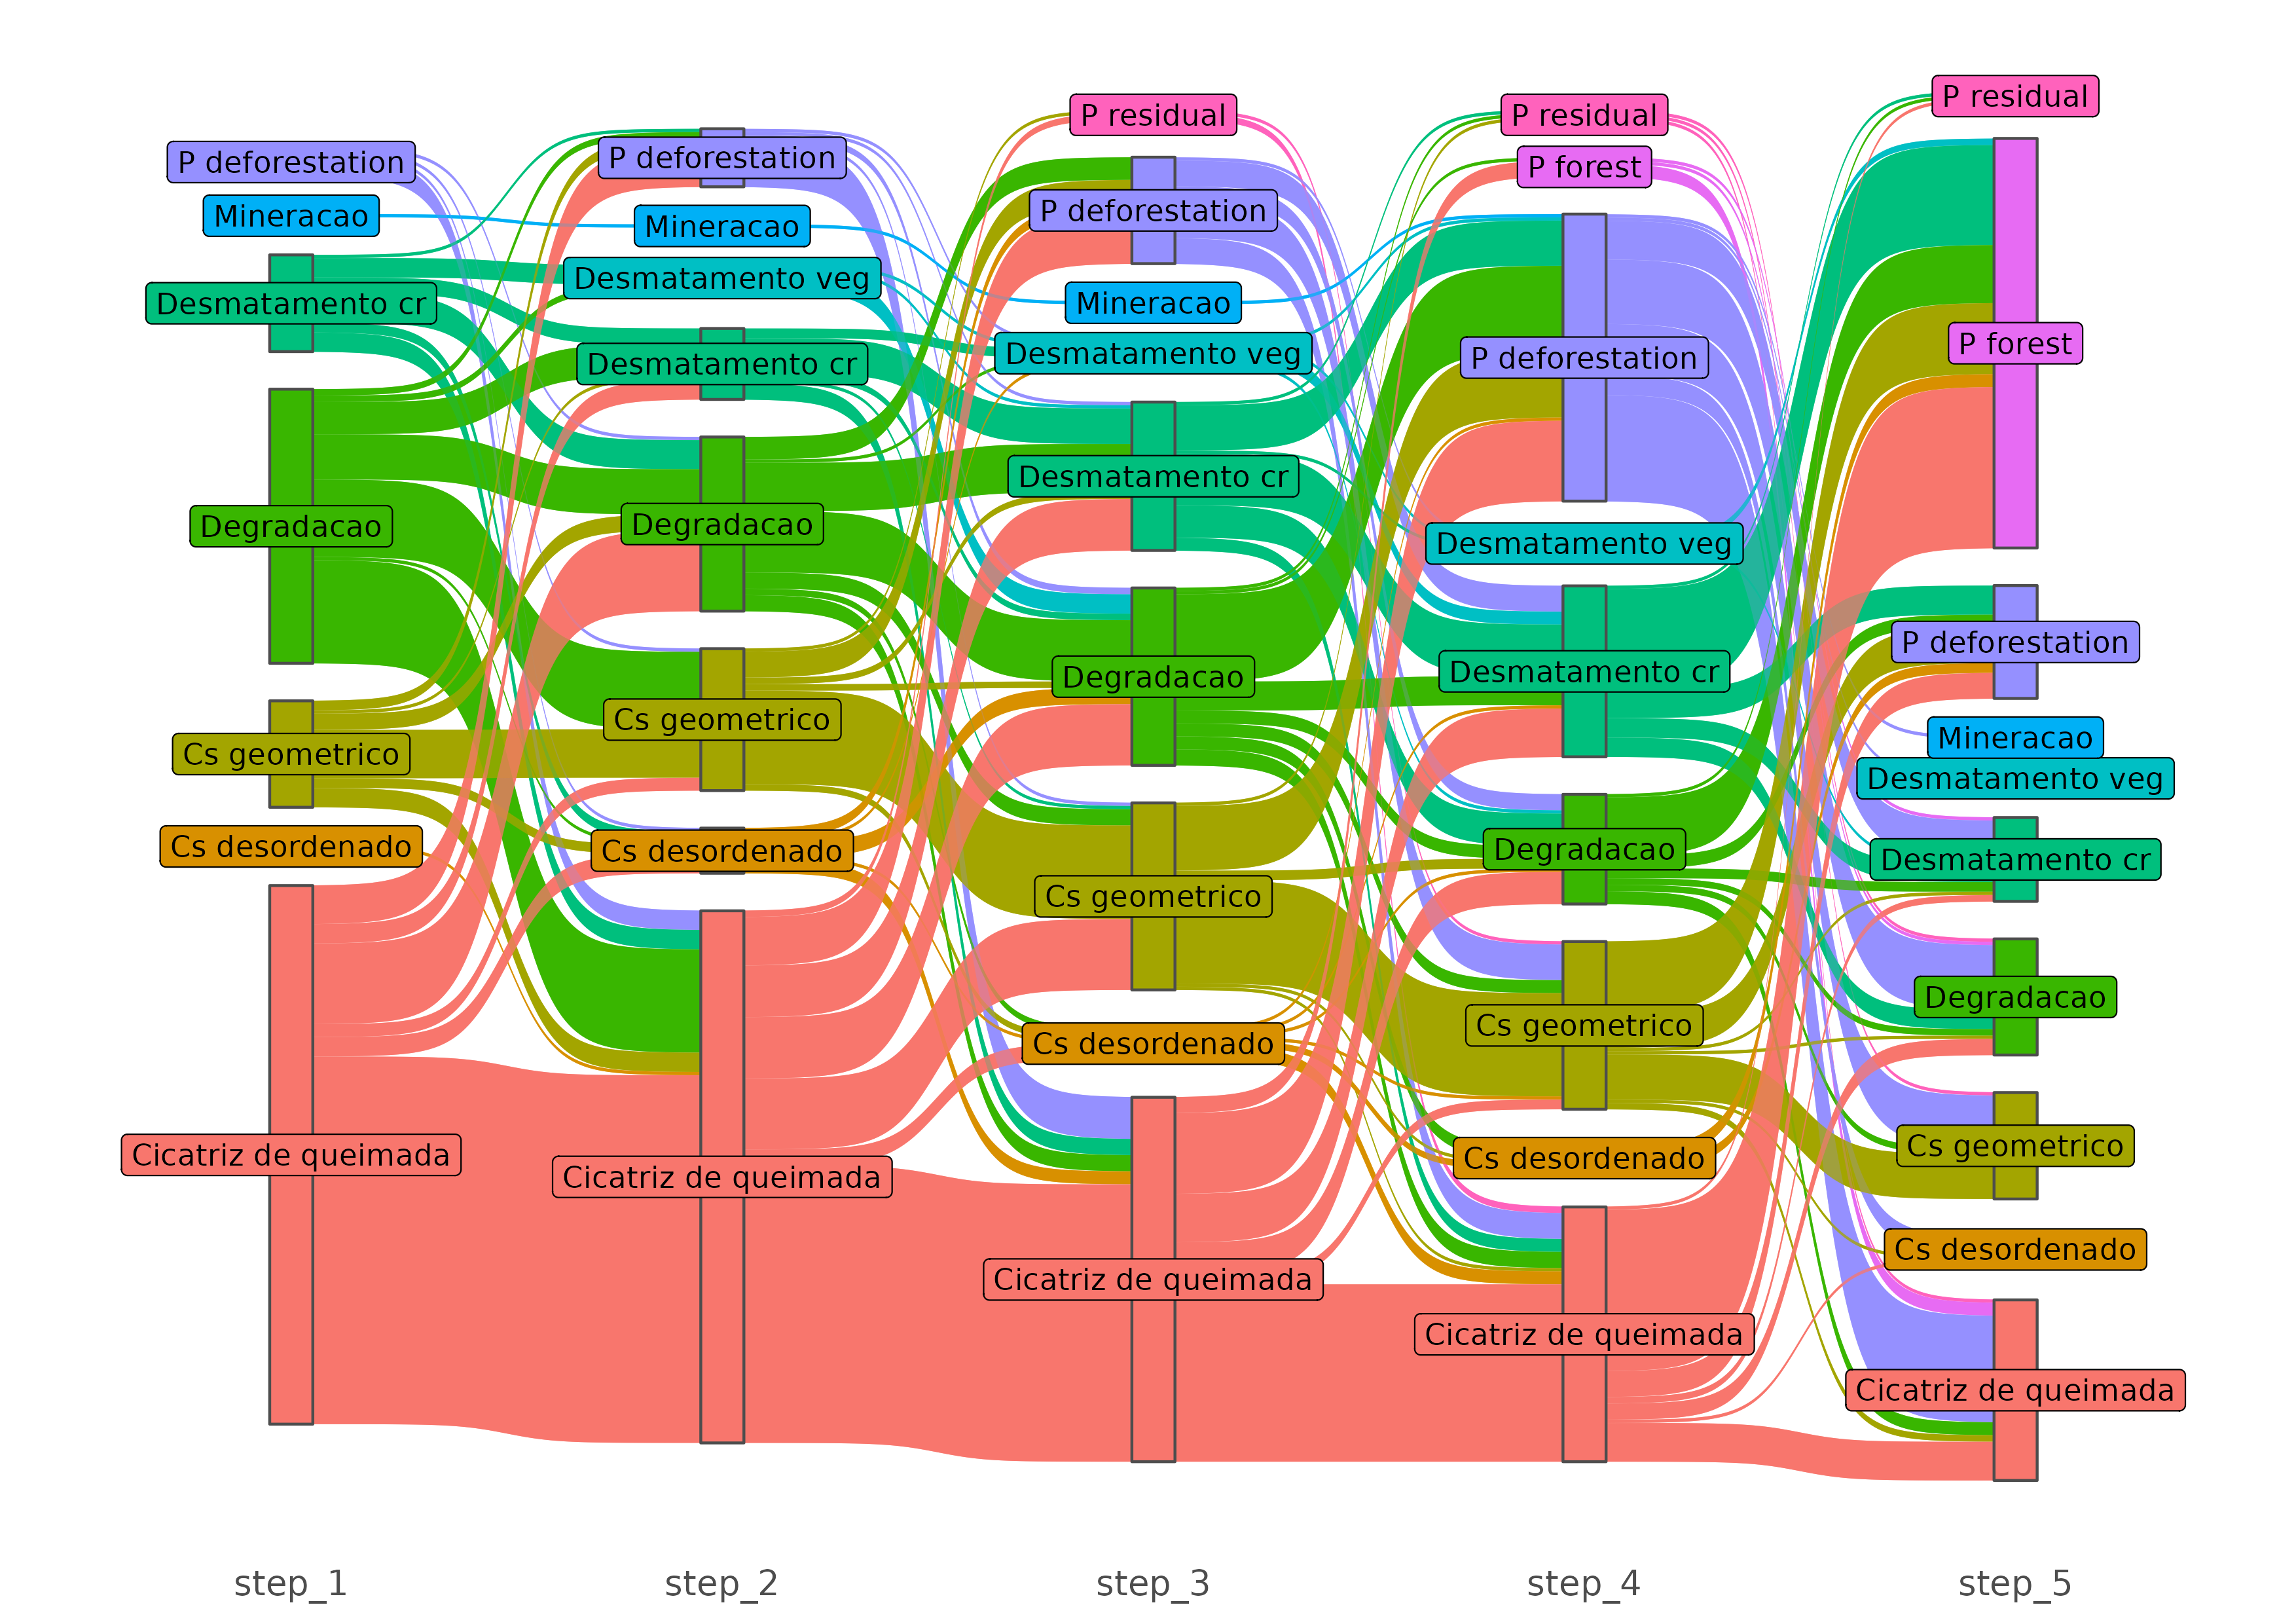
\includegraphics[width=0.65\linewidth]
        {./figures/plot_deter_prodes_subarea_trajectory_5.png}
        \caption{Tajectory of subareas with 5 wanings.}
        \label{fig:deter_prodes_subarea_trajectory_5}
    \end{figure}
\end{frame}

\begin{frame}[allowframebreaks]
    \frametitle{DETER \& PRODES - Top 10 trajectories (5 warnings)}
    \begingroup\fontsize{7}{9}\selectfont

\begin{longtabu} to \linewidth {>{\raggedright}X>{\raggedright}X>{\raggedright}X>{\raggedright}X>{\raggedright}X>{\raggedleft}X>{\raggedleft}X>{\raggedleft}X>{\raggedleft}X}
\toprule
position\_1 & position\_2 & position\_3 & position\_4 & position\_5 & area\_ha & n\_traj & p\_area & p\_traj\\
\midrule
\cellcolor{gray!6}{Cicatriz de queimada} & \cellcolor{gray!6}{Cicatriz de queimada} & \cellcolor{gray!6}{Cicatriz de queimada} & \cellcolor{gray!6}{Cicatriz de queimada} & \cellcolor{gray!6}{P forest} & \cellcolor{gray!6}{1290.8} & \cellcolor{gray!6}{33} & \cellcolor{gray!6}{14.6} & \cellcolor{gray!6}{10.1}\\
\cmidrule{1-9}
Cicatriz de queimada & Cicatriz de queimada & Cicatriz de queimada & P deforestation & Cicatriz de queimada & 384.5 & 14 & 4.3 & 4.3\\
\cmidrule{1-9}
\cellcolor{gray!6}{Cicatriz de queimada} & \cellcolor{gray!6}{Cicatriz de queimada} & \cellcolor{gray!6}{Cicatriz de queimada} & \cellcolor{gray!6}{Cicatriz de queimada} & \cellcolor{gray!6}{P deforestation} & \cellcolor{gray!6}{364.5} & \cellcolor{gray!6}{8} & \cellcolor{gray!6}{4.1} & \cellcolor{gray!6}{2.5}\\
\cmidrule{1-9}
Cicatriz de queimada & P deforestation & Cicatriz de queimada & Cicatriz de queimada & Degradacao & 308.7 & 3 & 3.5 & 0.9\\
\cmidrule{1-9}
\cellcolor{gray!6}{Degradacao} & \cellcolor{gray!6}{Cs geometrico} & \cellcolor{gray!6}{Cs geometrico} & \cellcolor{gray!6}{Cicatriz de queimada} & \cellcolor{gray!6}{P forest} & \cellcolor{gray!6}{279.9} & \cellcolor{gray!6}{1} & \cellcolor{gray!6}{3.2} & \cellcolor{gray!6}{0.3}\\
\cmidrule{1-9}
Total & - & - & - & - & 8845.8 & 326 & 100.0 & 100.0\\
\bottomrule
\end{longtabu}
\endgroup{}
\end{frame}

\begin{frame}
    \frametitle{DETER \& PRODES subareas (6 warnings)}
    \begin{figure}[h] 
        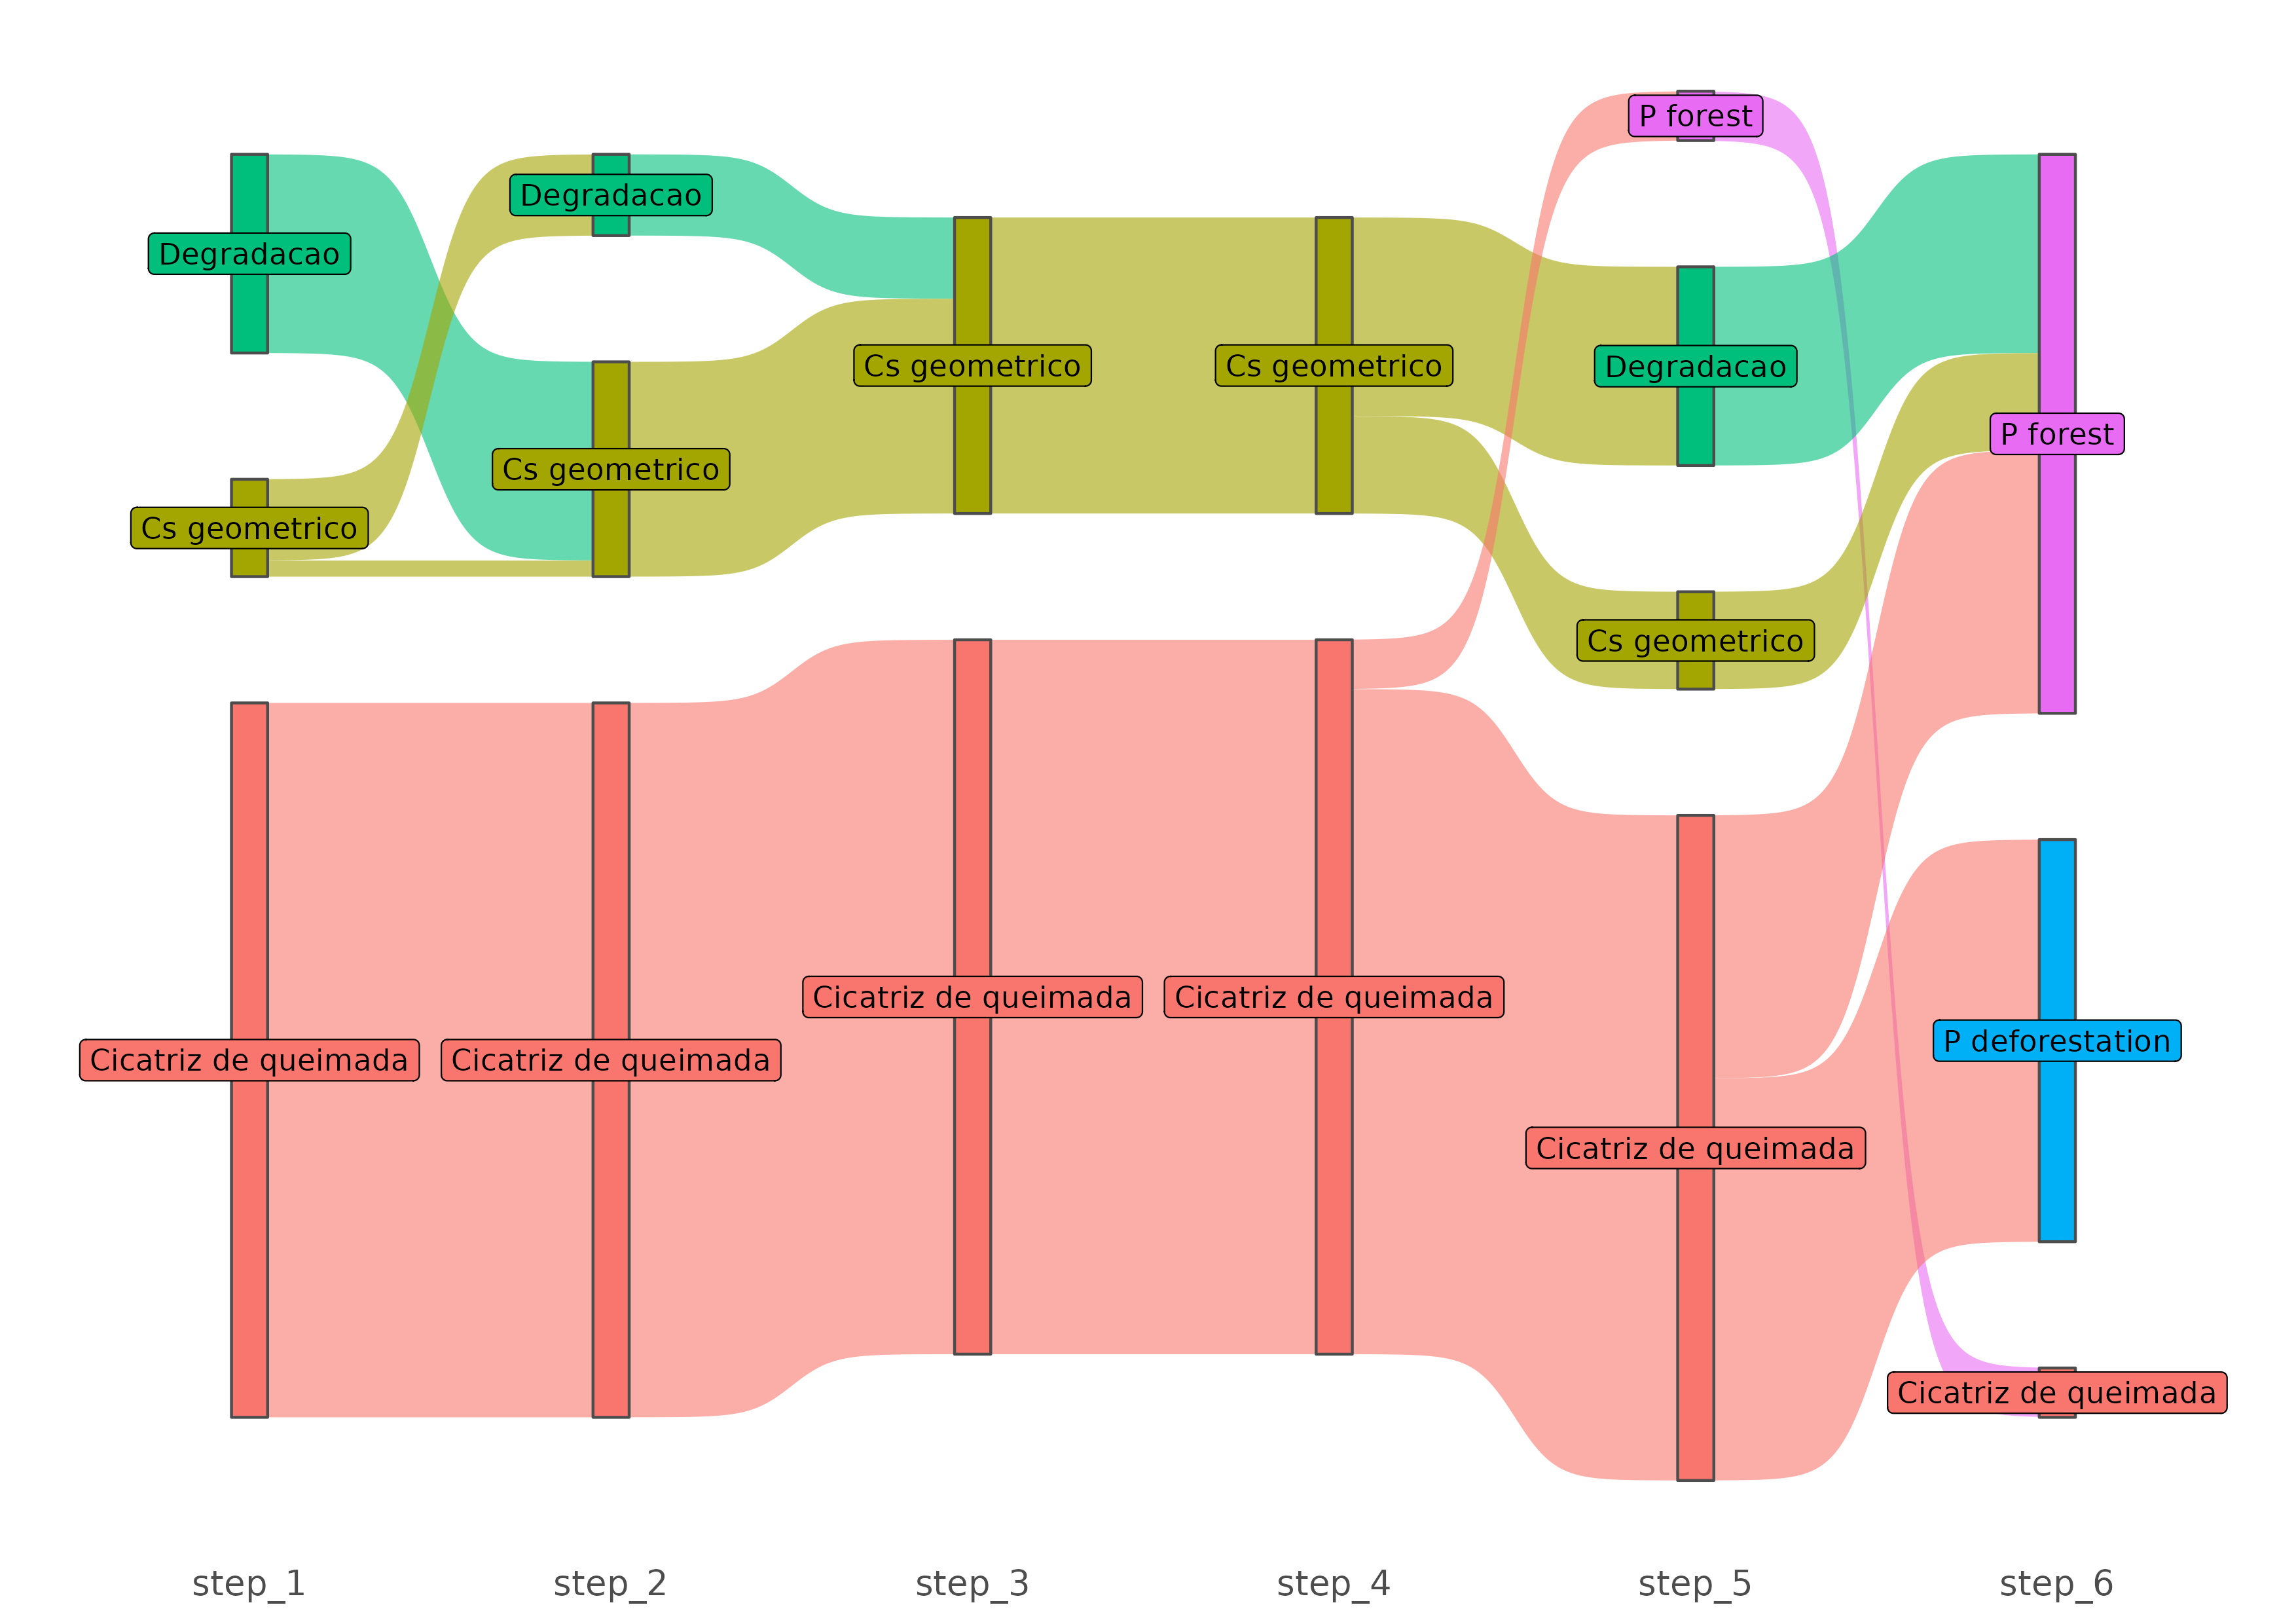
\includegraphics[width=0.65\linewidth]
        {./figures/plot_deter_prodes_subarea_trajectory_6.png}
        \caption{Tajectory of subareas with 6 wanings.}
        \label{fig:deter_prodes_subarea_trajectory_6}
    \end{figure}
\end{frame}

\begin{frame}[allowframebreaks]
    \frametitle{DETER \& PRODES - Top 10 trajectories (6 warnings)}
    \begingroup\fontsize{7}{9}\selectfont

\begin{longtabu} to \linewidth {>{\raggedright}X>{\raggedright}X>{\raggedright}X>{\raggedright}X>{\raggedright}X>{\raggedright}X>{\raggedleft}X>{\raggedleft}X}
\toprule
position\_1 & position\_2 & position\_3 & position\_4 & position\_5 & position\_6 & area\_ha & n\_traj\\
\midrule
\cellcolor{gray!6}{Cicatriz de queimada} & \cellcolor{gray!6}{Cicatriz de queimada} & \cellcolor{gray!6}{Cicatriz de queimada} & \cellcolor{gray!6}{Cicatriz de queimada} & \cellcolor{gray!6}{Cicatriz de queimada} & \cellcolor{gray!6}{P forest} & \cellcolor{gray!6}{187.4} & \cellcolor{gray!6}{4}\\
\cmidrule{1-8}
Degradacao & Cs geometrico & Cs geometrico & P deforestation & Cs geometrico & Degradacao & 74.3 & 1\\
\cmidrule{1-8}
\cellcolor{gray!6}{Cicatriz de queimada} & \cellcolor{gray!6}{Cicatriz de queimada} & \cellcolor{gray!6}{P deforestation} & \cellcolor{gray!6}{Cicatriz de queimada} & \cellcolor{gray!6}{Cicatriz de queimada} & \cellcolor{gray!6}{Cicatriz de queimada} & \cellcolor{gray!6}{55.7} & \cellcolor{gray!6}{2}\\
\cmidrule{1-8}
Cicatriz de queimada & Cicatriz de queimada & Cicatriz de queimada & Cicatriz de queimada & P deforestation & Cicatriz de queimada & 30.4 & 3\\
\cmidrule{1-8}
\cellcolor{gray!6}{Cs geometrico} & \cellcolor{gray!6}{Degradacao} & \cellcolor{gray!6}{Cs geometrico} & \cellcolor{gray!6}{P deforestation} & \cellcolor{gray!6}{Cs geometrico} & \cellcolor{gray!6}{Cs geometrico} & \cellcolor{gray!6}{21.9} & \cellcolor{gray!6}{1}\\
\cmidrule{1-8}
Total & - & - & - & - & - & 369.7 & 11\\
\bottomrule
\end{longtabu}
\endgroup{}
\end{frame}

\begin{frame}[allowframebreaks]
    \frametitle{DETER \& PRODES - Top 10 proximity in time}
    \begingroup\fontsize{7}{9}\selectfont

\begin{longtabu} to \linewidth {>{\raggedright}X>{\raggedright}X>{\raggedleft}X>{\raggedleft}X>{\raggedleft}X>{\raggedleft}X>{\raggedleft}X>{\raggedleft}X}
\toprule
CLASSNAME & closest\_class & total\_ha & n & median\_days & median\_days\_abs & sd\_days & sd\_abs\\
\midrule
\cellcolor{gray!6}{P desmatamento} & \cellcolor{gray!6}{Cicatriz de queimada} & \cellcolor{gray!6}{1620833.2} & \cellcolor{gray!6}{26272} & \cellcolor{gray!6}{300} & \cellcolor{gray!6}{396} & \cellcolor{gray!6}{687.2} & \cellcolor{gray!6}{496.9}\\
P forest 2021 & Cicatriz de queimada & 1338484.8 & 19411 & 688 & 688 & 516.1 & 515.8\\
\cellcolor{gray!6}{P desmatamento} & \cellcolor{gray!6}{Desmatamento cr} & \cellcolor{gray!6}{1049533.4} & \cellcolor{gray!6}{57922} & \cellcolor{gray!6}{64} & \cellcolor{gray!6}{383} & \cellcolor{gray!6}{731.8} & \cellcolor{gray!6}{504.0}\\
P forest 2021 & Desmatamento cr & 939836.4 & 47172 & 649 & 649 & 488.8 & 488.4\\
\cellcolor{gray!6}{P desmatamento} & \cellcolor{gray!6}{Degradacao} & \cellcolor{gray!6}{391152.0} & \cellcolor{gray!6}{11266} & \cellcolor{gray!6}{353} & \cellcolor{gray!6}{478} & \cellcolor{gray!6}{731.9} & \cellcolor{gray!6}{511.0}\\
P forest 2021 & Degradacao & 303475.8 & 8198 & 1028 & 1028 & 540.6 & 540.4\\
\cellcolor{gray!6}{P desmatamento} & \cellcolor{gray!6}{Cs desordenado} & \cellcolor{gray!6}{218994.5} & \cellcolor{gray!6}{1861} & \cellcolor{gray!6}{11} & \cellcolor{gray!6}{364} & \cellcolor{gray!6}{746.3} & \cellcolor{gray!6}{531.8}\\
P forest 2021 & Cs desordenado & 194497.7 & 1526 & 401 & 401 & 530.4 & 530.0\\
\cellcolor{gray!6}{P desmatamento} & \cellcolor{gray!6}{Cs geometrico} & \cellcolor{gray!6}{168756.0} & \cellcolor{gray!6}{1658} & \cellcolor{gray!6}{44} & \cellcolor{gray!6}{348} & \cellcolor{gray!6}{636.2} & \cellcolor{gray!6}{464.5}\\
P forest 2021 & Cs geometrico & 130931.0 & 1155 & 379 & 379 & 473.8 & 473.6\\
\bottomrule
\end{longtabu}
\endgroup{}
\end{frame}




\section{Closing}

\begin{frame}
    \frametitle{Final remarks}
    \begin{itemize}
        \item The analysis of DETER warning subareas along time could improve 
            the characterization of forest degradation along time.
        \item Potential applications of our work are:
            \begin{itemize}
                \item Improve estimation of emissions of greenhouse gases, i.e.
                    our data could help avoiding double counting.
                \item Identify spatio-temporal areas which could help training 
                    Machine-Learning algorithms for automatic indentification 
                    of forest degradation.
            \end{itemize}
        \item Code available at 
            \url{https://github.com/albhasan/treesburnareas}
    \end{itemize}
\end{frame}

\begin{frame}[allowframebreaks]
    \frametitle{References}
    \bibliographystyle{amsalpha}
    \bibliography{07_SBSR.bib}
\end{frame}

\end{document}
